\documentclass[12pt]{article}
\usepackage[utf8]{inputenc}
\usepackage{enumitem}
%\usepackage[spanish]{babel}
\usepackage[spanish,es-tabla]{babel}
%\usepackage[T1]{fontenc}
\usepackage{lmodern}
\usepackage{graphicx}
\usepackage{pdfpages}
\usepackage{url}
\usepackage{float}
\usepackage[lmargin=3cm,rmargin=3cm,top=2.5cm,bottom=2.5cm]{geometry}
\usepackage{fancyvrb}
\usepackage{fancyhdr}
\usepackage{titlesec}
\usepackage{amsmath}
\usepackage{hyperref}
\usepackage{datetime}
\usepackage{hyperref}
\usepackage{textcomp}
\usepackage{listings}
\usepackage{amsmath, amsthm, amssymb, tabu}
\usepackage{array}
\usepackage{multicol}
\usepackage{hyperref}
\usepackage{breakurl}
\usepackage[T1]{fontenc}
\usepackage{color}
\usepackage{tocloft} % Añadido el paquete tocloft
\definecolor{codegreen}{rgb}{0,0.6,0}
\definecolor{backcolour}{rgb}{0.95,0.95,0.92}
\definecolor{gray}{rgb}{0.5, 0.5, 0.5}

\lstdefinestyle{mystyle}{
    backgroundcolor=\color{backcolour},   
    commentstyle=\color{codegreen}\ttfamily,
    keywordstyle=\bfseries\color{blue},
    numberstyle=\tiny\color{gray},
    stringstyle=\ttfamily\color{red},
    basicstyle=\ttfamily\footnotesize,
    breakatwhitespace=false,         
    breaklines=true,                 
    captionpos=b,                    
    keepspaces=true,                 
    %numbers=left,                    
    %numbersep=5pt,                  
    showspaces=false,                
    showstringspaces=false,
    showtabs=false,                  
    tabsize=2
}

\lstset{style=mystyle}


\pagestyle{fancy}

\hypersetup{
    colorlinks,
    citecolor=black,
    filecolor=black,
    linkcolor=black,
    urlcolor=blue
}

\fancyfoot{}
\setlength{\headheight}{15.71667pt}
\renewcommand{\footrulewidth}{0.5pt}
\fancyfoot[R]{\thepage}

\setcounter{secnumdepth}{3}

\titleformat{\paragraph}
{\normalfont\normalsize\bfseries}{\theparagraph}{1em}{}
\titlespacing*{\paragraph}
{0pt}{3.25ex plus 1ex minus .2ex}{1.5ex plus .2ex}

\newcommand{\subsubsubsection}[1]{\paragraph{#1}}

% Redefine el nombre del índice
\addto\captionsspanish{\renewcommand{\contentsname}{Índice general}}
\begin{document}

\begin{titlepage}
    \begin{center}

        {\phantom{a}\par}

        
\includegraphics[width=0.6\textwidth]{imagenes/logo.jpg}
        %\vspace*{1cm}

        \scshape\Large\textbf{UNIVERSIDAD DE MURCIA}
        \\\scshape\Large Facultad de Informática

        \rule{\linewidth}{0.1pt}
        \rule{\linewidth}{0.1pt}

        \vspace{1cm}
        \scshape\huge\textbf{App para pedidos de impresión}\\
        \scshape\Large Trabajo de fin de grado


        \vspace{1cm}

        \itshape\large
        Rubén Sánchez Fernández\\
        21067018F\\

        \vspace{0.5cm}
        \textbf{Tutor académico}\\
        \itshape\large
        Francisco García Sánchez\\
        \textbf{Tutor empresa}\\
        \itshape\large
        Carmela Pozuelo Monfort\\
        \vspace{0.5cm}


        \vfill
        {\large Convocatoria de Junio 2024}
    \end{center}
\end{titlepage}

\pagestyle{empty}
\pagenumbering{roman} % Números romanos para la primera parte
\setcounter{page}{1}
\part*{}
\tableofcontents
% Agrega un espacio en el índice
\addtocontents{toc}{\vspace{\baselineskip}}
\newpage
\listoffigures
\newpage
\clearpage
\pagestyle{fancy}

% 
\includepdf[pages=1]{Anexo_V_VistoBueno_Empresa_Ruben_firmado.pdf}

\includegraphics[width=1\textwidth]{Anexo_Firmado_Upango.png}

\clearpage
\section{Resumen}
Este es el resumen…
ESTILO DE REDACCIÓN APLICABLE A TODO EL DOCUMENTO: evitaremos el uso de la primera persona; en su lugar se suele emplear el reflexivo (“hemos desarrollado” “se ha desarrollado”).

\clearpage

\section{Extended abstract}
Resumen extendido en inglés (2000 palabras). En el abstract conviene replicar de algún modo la estructura de la memoria en sí: (i) introducción, (ii) estado del arte, (iii) objetivos y metodología, (iv) diseño y resolución del trabajo, (v) conclusiones y trabajo futuro. El contenido del abstract tiene que abarcar todos esos conceptos en ese orden.

% Fin de la primera parte
\cleardoublepage

\part*{}
\pagenumbering{arabic} % Números arábigos para la segunda parte
\setcounter{page}{1} % Reinicia el contador de página

\section{Introducción}
Esto se escribe lo último, junto con el resumen y el abstract. Se establece el contexto en el que se sitúa el proyecto introduciendo claramente la problemática e indicando el objetivo general del proyecto (como consecuencia de esos problemas que se quieren resolver). Suele venir acompañado de numerosas referencias bibliográficas relevantes sobre los distintos conceptos tratados. En el último párrafo de la introducción hay que indicar la estructura/organización del resto del documento (un párrafo indicando brevemente en qué secciones se ha dividido el documento y el contenido de cada sección).

\clearpage
\section{Estado del arte}
En este apartado se expondrá por un lado el contexto inicial y la situación de partida junto con el problema a solucionar que se plantea y por 
otro lado se realizará un análisis de las herramientas y tecnologías que se han decidido emplear para el desarrollo de la solución al problema.
\subsection{Contexto y análisis de la situación de partida}
Este Trabajo de Fin de Grado (TFG) ha sido desarrollado en colaboración con Upango, empresa especializada en transformaciones digitales B2B.
Durante años ha trabajado con uno de los proveedores de soluciones de tiendas online más populares del mundo como es ePages \cite{epages},
desarrollando aplicaciones y tiendas online a medida para los clientes en el ámbito del comercio electrónico. A lo largo del tiempo,
se ha observado en esta empresa, una creciente demanda de incorporar al desarrollo de tiendas personalizadas, funcionalidades que permitan a los clientes
personalizar los productos para su posterior compra; es decir en el mercado actual hay una gran cantidad de clientes potenciales que podrían solicitar desarrollos de comercio
electrónico a medida con funcionalidades de personalización de productos.

Recientemente se ha decidido migrar de ePages a otra plataforma de comercio electrónico como es Shopify \cite{shopify} que ofrece otras tecnologías y herramientas
para el desarrollo personalizado de tiendas online. Debido a esta migración, los desarrollos a medida y aplicaciones estandarizadas de la otra plataforma quedan obsoletas para nuevos desarrollos
y surge la necesidad de adaptarse a estas nuevas herramientas y funcionalidades que proporciona Shopify para conseguir crear estos desarrollos de comercio a medida. Por lo que, si
bien en las tiendas de ePages de los actuales clientes existen ya desarrollos y funcionalidades para la personalización de artículos, la transición a Shopify requiere la creación de
una nueva solución y adaptación para esta plataforma.

Debido a la necesidad que se crea propulsada por este gran cambio, el objetivo que se persigue con este proyecto es crear una aplicación para la plataforma Shopify que sea versátil y escalable,
y permita integrarse en las tiendas de los nuevos clientes para ofrecerles la capacidad de proporcionar experiencias de compra de productos personalizados,
manteniendo el compromiso con la excelencia en el desarrollo de soluciones digitales para comercio electrónico.

\subsection{Herramientas y tecnologías empleadas}
En el desarrollo de aplicaciones web modernas, concretamente en la creación de tiendas personalizadas, la selección de los proveedores de soluciones
y las tecnologías apropiadas desempeña un papel fundamental para garantizar el desarrollo de soluciones efectivas y personalizadas para los clientes.
En este contexto, la decisión más trascendental ha sido la de seleccionar el mejor proveedor de soluciones, en este caso \textbf{Shopify}.

Es importante destacar que la elección de parte de las tecnologías ha estado fuertemente influenciada por la decisión de la empresa de emplear Shopify
como base para sus desarrollos. Debido a esto la búsqueda de las tecnologías necesarias para desarrollar el proyecto se han limitado a
tecnologías que se integran y están aceptadas sin problemas con la plataforma para conseguir aprovechar al máximo sus capacidades. Shopify es una plataforma que está en continua mejora y crecimiento y no se queda atrás en cuanto a las tecnologías.

La plataforma Shopify, con su amplia gama de herramientas y funcionalidades para el comercio electrónico, 
proporciona una base sólida para el desarrollo de tiendas en línea personalizadas. Originaria de Canadá y 
fundada en 2006, esta se ha convertido en uno de los proveedores líderes en el mercado de comercio electrónico, 
atendiendo a millones de comerciantes en todo el mundo. 

Cuenta con multitud de ventajas frente a otras plataformas de comercio electrónico muy populares en el mercado. Una de las ventajas
mas trascendentales y que ha influenciado fuertemente  la decisión de Upango de migrar de \textbf{ePages} a esta tecnología, es el hecho de que Shopify elimina
las barreras iniciales al ofrecer un servicio completo que incluye registro de dominio y hosting web ilimitado. Esto simplifica el proceso de lanzamiento y mantenimiento
de una tienda al eliminar la necesidad de buscar proveedores de hosting externos, además de dotar a los usuarios de tecnologías avanzadas como servidores de alta
calidad, redes optimizadas y un CDN global para garantizar una velocidad de carga rápida \cite{shopify-tutorial}. Esto no solo mejora la experiencia del usuario, sino que también 
tiene un impacto positivo en el posicionamiento SEO y en la tasa de conversión. Cabe destacar que Shopify cuenta con una tasa de conversión de las más
elevadas del mercado \cite{shopify-tasa-conversion}. 

Una de las características con las que cuenta Shopify, es la habilidad de poder crear aplicaciones que puedan ampliar las capacidades existentes 
de esta plataforma. Esto permite agregar funcionalidades a las tiendas, ampliar la experiencia de la parte de administración
o crear experiencias de compra únicas para los clientes. Gracias a esto los usuarios pueden instalar estas aplicaciones para ayudar a desarrollar
su negocio, integrarse con servicios externos y agregar funciones a su panel de control de Shopify \cite{shopify-dev}. 

\subsubsection{Frontend}
En cuanto al frontend de la aplicación se pueden observar dos partes. 
Por un lado se puede encontrar el frontend asociado a la parte de administración de Shopify. 
Esta parte hace referencia a la interfaz del usuario que los administradores de la tienda emplean para gestionar y controlar los diversos aspectos de
la misma, como la gestión de productos, pedidos, clientes, configuración de temas, traducciones y otros muchos aspectos de configuración de la tienda.
Al instalar la aplicación en las tiendas que necesiten de sus funcionalidades esta parte del frontend se integrará con la página de administración de 
cada tienda, proporcionando la interfaz y las funcionalidades que se configuren en esta parte del desarrollo. En la Figura~\ref{fig:1} se puede observar la 
interfaz de administración de una tienda Shopify en desarrollo.

\begin{figure}[ht]
    \floatplacement{figure}{!t}
    \centering
    \includegraphics[width=0.8\textwidth]{imagenes/Interfaz de administración.png}
    \caption{\label{fig:1}Interfaz de administración de tienda Shopify}
    \vspace{\fill}
\end{figure}

Esta parte del frontend ha sido desarrollada empleando la biblioteca de JavaScript \textbf{React} \cite{react-pag-1}. Se trata de una libería de código abierto creada por el equipo de la
compañia Facebook (Meta) junto a una gran comunidad de desarrolladores independientes que, desde su lanzamiento en 2013, se ha convertido en una
de las tecnologías de frontend más usadas, ya que permite construir interfaces de usuario dinámicas y escalables. Esta se usa en el desarrollo de aplicaciones web y móviles. 

Toda aplicación web React, se compone de componentes reutilizables que conforman partes de la interfaz de usuario. Permite tener un componente distinto para
la barra de navegación, otro para el pie de página, otro para el contenido principal, etc.
Tener estos componentes reutilizables facilita el desarrollo ya que no es necesario repetir el código reiterativo, solo habría que crear su lógica e
importar el componente en cualquier parte del código donde se necesite. Estos componentes representan una fusión de la estructura \textbf{HTML} \cite{html} con la funcionalidad de \textbf{JavaScript} \cite{javascript}.
React también conforma una aplicación de una sola página, por tanto, en lugar de enviar una petición al servidor cada vez que hay que renderizar una nueva página,
el contenido de la misma se carga directamente desde los componentes de React conduciendo de este modo a una renderización más rápida sin recargas de página. \cite{react-pag-2}

Para la integración de la aplicación con el panel de administración de las tiendas Shopify se ha hecho uso de \textbf{App Bridge} \cite{app-bridge}, una biblioteca de JavaScript
desarrollada por Shopify que permite a los desarrolladores integrar las aplicaciones personalizadas para las tiendas. Se trata de una interfaz
de programación diseñada para facilitar la comunicación entre la tienda y las aplicaciones externas, que proporciona herramientas y funcionalidades
que permiten a los desarrolladores que sus aplicaciones se integren de forma nativa en el panel de administración y en la experiencia de compra
del cliente. De esta forma se proporciona la capacidad de acceder a datos de la tienda como productos, pedidos y clientes, así como la capacidad de interactuar con la interfaz
de usuario de la tienda agregando componentes y paneles personalizados \cite{shopify-dev}. 

Además se ha empleado el sistema de diseño \textbf{Polaris} \cite{polaris}, una biblioteca de React que define los componentes necesarios para el panel de administración.
El panel de control de Shopify proporciona una superficie para que las aplicaciones integradas rendericen su interfaz de usuario, y el empleo de Polaris
es fundamental para crear experiencias de usuario familiares y coherentes.
Polaris incluye una guía de diseño, con instrucciones sobre accesibilidad, colores, tipografía, espaciado, nomenclatura y lenguaje práctico para ayudar 
a crear experiencias que se parezcan al resto del panel de administración. Proporciona componentes, es decir bloques de construcción reutilizables compuestos de 
elementos y estilos de interfaz empaquetados a través de código. Además proporciona tokens, es decir valores CSS con nombre que representan decisiones
de diseño para elementos como el color, el espaciado y la tipografía se puede aplicar a los diseños para ayudar a unificar las experiencias de los usuarios.
También proporciona iconos cuidadosamente diseñados que se centran en el comercio y el emprendimiento, que se pueden emplear como ayudas visuales para ayudar a los 
usuarios a completar tareas. Y por último proporciona patrones, soluciones repetibles a problemas comunes de experiencia de usuario (UX, en ingles "User eXperience") en una situación expecífica del usuario
El buen uso de estos patrones hace que el panel de administración sea familiar y facil de usar \cite{shopify-dev}.

La otra parte del frontend de esta aplicación, es la extensión del tema de la tienda. Un tema en Shopify es un conjunto de recursos
y archivos que determinan la apariencia, funcionalidad y sensación de una tienda en línea en esta plataforma, tanto para los comerciantes como para
sus clientes \cite{theme}. Estos temas se construyen empleando un lenguaje de plantillas llamado \textbf{Liquid} \cite{liquid} que, junto con \textbf{HTML}, \textbf{CSS} y \textbf{JavaScript}, conforman la apariencia
y funcionalidades del frontend de la tienda online. Los desarrolladores pueden crear temas personalizados para las tiendas y ajustar los temas existentes 
para adaptarse a las necesidades de los comerciantes \cite{shopify-dev}. 

Los administradores tienen la posibilidad de elegir entre varios temas para aplicar a su tienda desde la propia interfaz de administración,
ya sean los temas que proporciona Shopify o temas desarrollados y personalizados por otros usuarios como es el caso de Upango. Estos temas pueden ser
configurados desde la interfaz de administración por los comerciantes.
En la Figura~\ref{fig:2} se muestra la pantalla de la interfaz de administración en la que aparece el tema seleccionado; además se puede observar una 
biblioteca de temas con otros temas sin publicar. También se puede destacar el botón de personalizar que aparece
sobre el tema que está activo; este abriría un editor que permitiría ajustar ciertos aspectos visuales y detalles funcionales del tema establecido.

\begin{figure}[ht]
    \floatplacement{figure}{!t}
    \centering
    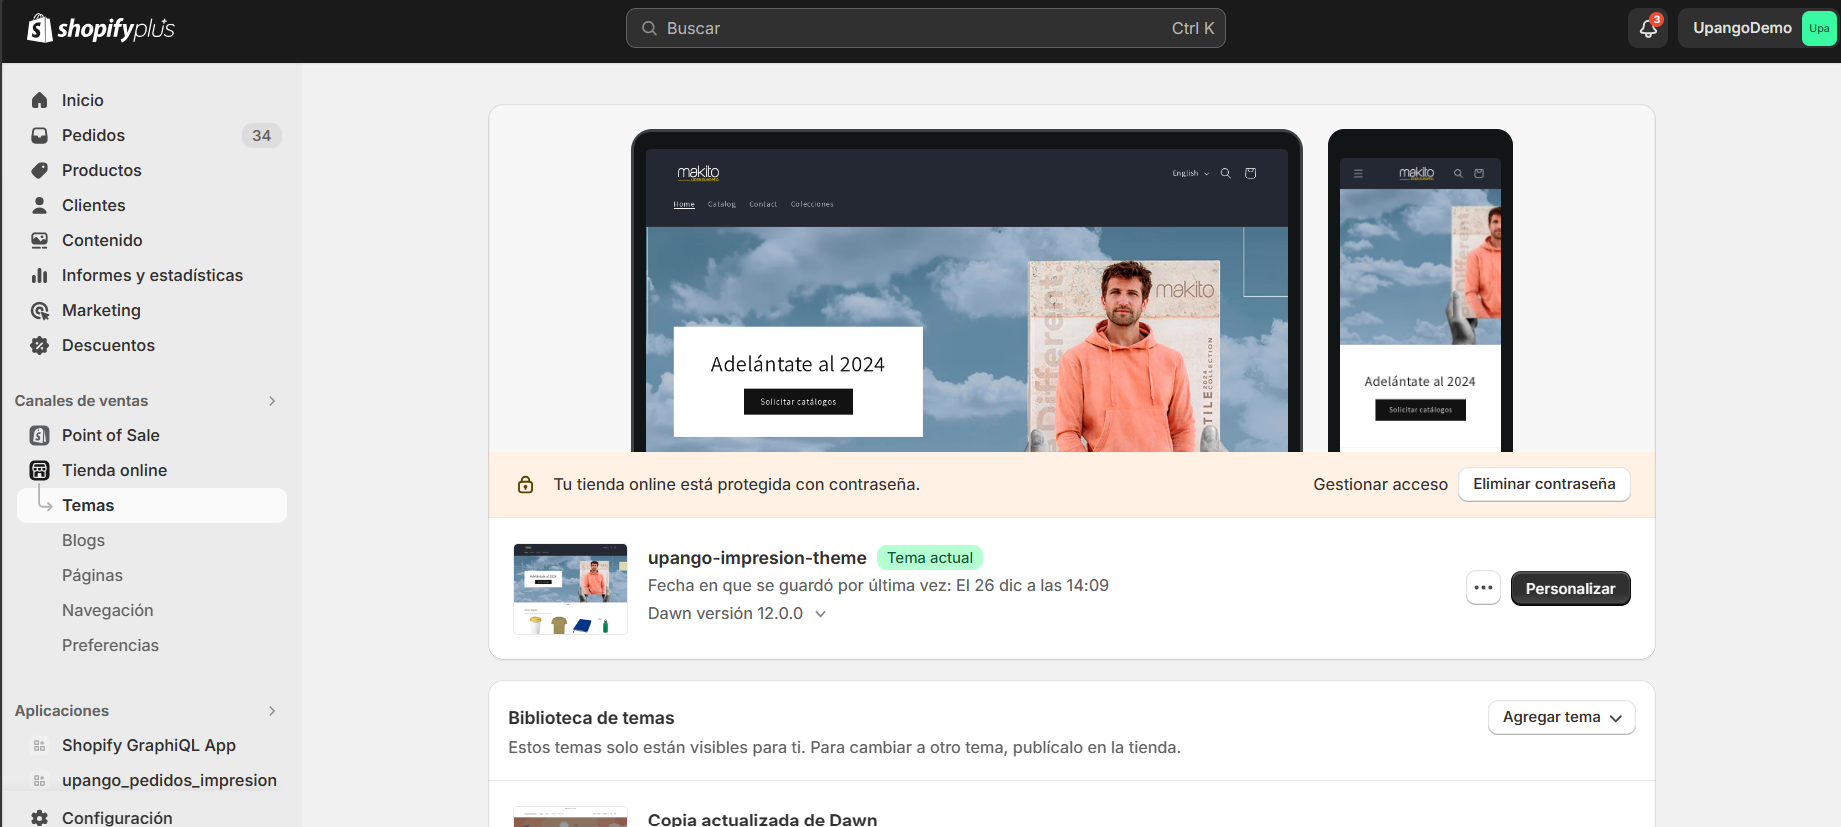
\includegraphics[width=0.8\textwidth]{imagenes/Interfaz de adminsitración elección de tema.png}
    \caption{\label{fig:2}Selección de tema en la interfaz de administración}
    \vspace{\fill}
\end{figure}

Para ampliar el tema de las tiendas en las que se instale la aplicación que se ha desarrollado y así poder dotarla de las funcionalidades de personalización de 
artículos, se ha creado en la aplicación lo que se conoce como \textbf{App Theme Extension} \cite{theme-app-extension}. Las extensiones de aplicaciones de temas permiten a los comerciantes
agregar fácilmente elementos dinámicos a sus temas sin tener que interactuar directamente con las plantillas o el código \textbf{Liquid} del tema. Estas extensiones
se integran con el tema de la tienda exponiendo automáticamente en el editor de temas las secciones y elementos que haya programados en la aplicación. \cite{shopify-dev}
Una de las ventajas de desarrollar estas partes del tema en la aplicación y no directamente en el tema de la tienda, es que las secciones de código y funcionalidades
que se progarmen en la aplicación pasarán a estar disponibles en el tema de la tienda en la que se instale directamente sin necesidad de tener que ir modificando el tema
de cada tienda en la que se necesite instalar la aplicación. Es decir, puede implementarse la aplicación al mismo tiempo en todas las tiendas que la usan,
sin necesidad de que los comerciantes tengan que editar manualmente el código del tema.

Los App Theme Extension tienen una estructura similar a los temas, ya que son como una prolongación de ellos. Estos contienen los siguientes recursos. 
los \textit{bloques}, son archivos en Liquid que actúan como punto de entrada para lo que se desea inyectar en un tema.
Recursos, contienen los ficheros CSS, JavaScript y otros contenidos estáticos de la aplicación que se insertan en los temas.
Los snippets, son fragmentos de código Liquid reutilizables que se pueden emplear en varios bloques. Por último, una estructura de archivos locales
para implementar un sistema de traducciones en los idiomas que se configuren \cite{shopify-dev}. 

Como se ha comentado anteriormente, para el desarrollo de estas interfaces del tema se emplea \textbf{Liquid}, un lenguaje de plantillas creado por Shopify que
permite crear una sola plantilla para alojar el contenido estático e insertar información dinámicamente en función de dónde se representa la plantilla.
Por ejemplo, se pueden crear plantillas de producto que alojen todos los atributos estándar de este, como la imagen, el título, el precio y demás, y esta 
plantilla puede representar dinámicamente esos atributos con el contenido adecuado en función del valor actual que se esté viendo \cite{shopify-dev}. 
Además, en las plantillas junto con Liquid se ha empleado \textbf{HTML}, \textbf{CSS} y \textbf{JavaScript} para completar el desarrollo de la extensión del tema. Se hace uso de HTML para estructurar
el contenido y crear elementos de las páginas, CSS para definir y dar estilos visuales a los elementos, y JavaScript para agregar la interactividad y la 
funcionalidad dinámica a la página. 

En el desarrollo frontend de la parte del tema, se ha hecho uso de una de las herramientas que proporciona Shopify, la \textbf{Shopify Ajax API} \cite{shopify-ajax-api}. La API de Ajax
proporciona un conjunto de puntos finales ligeros para el desarrollo de temas: permite agregar productos al carrito y actualizar el contador
de artículos del mismo, mostrar recomendaciones de productos relaccionados, sugerir productos y colecciones a los visitantes a medida que escriben
en un campo de búsqueda y una larga lista de funcionalidades que serán útiles para interactuar con la tienda \cite{shopify-dev}.

\subsubsection{Backend}
En cuanto al Backend de la aplicación se ha hecho uso de \textbf{Node.js} \cite{node}. Node es un entorno que trabaja en tiempo de ejecución, de código abierto, multi-plataforma, 
que permite a los desarrolladores crear toda clase de herramientas del lado del servidor y aplicaciones en \textbf{JavaScript}. 
Además proporciona un gran numero de ventajas. 

\begin{itemize}
\item Ofrece un gran rendimiento, pues ha sido diseñado específicamente para optimizar el rendimiento y la
escalabilidad en aplicaciones web, lo que lo convierte en un excelente complemento para resolver problemas comunes de desarrollo web como aplicaciones
en tiempo real. 
\item Todo el código se escribe en JavaScript, lo que simplifica trabajo y ahorra tiempo al no tener que preocuparse por las conmutaciones
de contexto entre diferentes lenguajes al escribir tanto el código del navegador como del servidor. 
\item JavaScript es un lenguaje relativamente nuevo y se beneficia de los avances en diseño de lenguajes en comparación con otros lenguajes tradicionales. 
\item \textbf{Node} cuenta con \textbf{NPM} (Node Packet Manager), un gestor de paquetes que proporciona acceso a una amplia gama de paquetes reutilizables, ofrece una excelente resolución de dependencias y permite automatizar
gran parte de la cadena de herramientas de compilación. 
\item Node es portable y compatible con multitud de sistemas operativos y está soportado por muchos proveedores de alojamiento web, contando con un gran ecosistema y una comunidad de desarrolladores muy activa. 
\item Por último, este entorno brinda muchas facilidades para crear servidores web básicos capaces de responder a cualquier solicitud empleando el paquete HTTP de Node y simplificando el proceso de desarrollo y despliegue de
aplicaciones Web \cite{node-express}.
\end{itemize}

Además se ha empleado \textbf{Express} \cite{express}, el framework web más popular de Node \cite{express-popular}, que simplifica enormemente el desarrollo de aplicaciones web al proporcionar
una serie de características esenciales. Con Express, los desarrolladores pueden escribir fácilmente manejadores de peticiones para diferentes 
verbos HTTP (esto es 'GET', 'POST', 'PUT', 'DELETE', etc.) en diversas rutas URL, integrar motores de renderización de vistas para generar respuestas dinámicas y establecer configuraciones de 
aplicaciones web de manera intuitiva. Además, permite la adición de procesamiento de middleware adicional en cualquier punto de la tubería de manejo de 
la petición, brindando flexibilidad y modularidad al desarrollo \cite{node-express}. 

En esta parte de la aplicación, se ha hecho uso de la API de administración \textbf{GraphQL} que proporciona Shopify \cite{api-administracion-graphql}. Esta consituye la principal forma en la que 
las aplicaciones pueden interactuar con la tienda, permitiendo leer y escribir la información de la tienda incluidos los productos, inventario, pedidos,
envíos y mucho más, y facilitando ampliar la funcionalidad existente de Shopify. Gracias a esta API es posible conectar el inventario
de la tienda con otros marketplaces, ofreciendo infinidad de posibilidades para incluir nuevas funcionalidades en el panel de control.
Esta API es compatible tanto con GraphQL como con REST aunque para este desarrollo se empleará GraphQL. Para interactuar con esta API las aplicaciones
deben autenticarse además de contar con los ámbitos de acceso pertinentes para acceder a los datos que se necesiten o se quieran modificar. \cite{shopify-dev}


\subsubsection{Otras tecnologías}
Para la elaboración de este TFG se ha empleado \textbf{Visual Studio Code} \cite{vsc} como entorno de desarrollo tanto para la creación de la aplicación como para
la redación del propio TFG en \textbf{LaTeX} \cite{latex}, empleando una serie de extensiones que han facilitado el trabajo. 
Se han aprovechado extensiones como Shopify Liquid Templates, Shopify Liquid, 
Polaris for VS Code, JavaScript (ES6), GraphQL, Latex Language support, Latex Workshop y ESLint para garantizar un desarrollo y documentación
fluida y eficaz. Estas extensiones han proporcionado una serie de funcionalidades como resaltado de sintaxis, autocompletado y validación de código, 
acceso rápido a la documentación, formateo de código y una serie de ventajas que han facilitado significativamente la creación y documentación de la aplicación.

Se ha empleado \textbf{Git} \cite{git} para llevar un control de versiones de la aplicación junto con \textbf{Azure DevOps} \cite{azure-devops}, una plataforma de Microsoft que ofrece una amplia
gama de características y funcionalidades que permiten a los equipos de desarrolo colaborar de manera efectiva en equipo y optimizar el proceso de desarrollo
de software. Esta herramienta ofrece gestión del código fuente, permitiendo almacenar y administrar el código fuente de nuestro proyecto en 
repositorios de código. También facilita la planificación, asignación y seguimiento de las tareas, problemas y requisitos del proyecto, haciendo
un seguimiento del trabajo, y muchas otras fucionalidades útiles para el desarrollo como seguimiento, pruebas y gestión del ciclo de vida de los proyectos \cite{devOps}. 

\clearpage
\section{Análisis de objetivos y metodología}
En esta sección se describen los objetivos que se persiguen con el desarrollo de este proyecto, así como la metodología empleada (tareas y temporalización) para alcanzar estos objetivos.

\subsection{Objetivos}

El objetivo principal de este TFG consiste en el análisis, diseño y desarrollo de una aplicación para la plataforma Shopify que permita
la personalización de productos para su posterior compra en las tiendas en las que se acople dicha aplicación. Para conseguir lograr este objetivo 
principal, se han propuesto los siguientes objetivos específicos.

\begin{enumerate}
    \item Estudiar las tecnologías y herramientas útiles para el desarrollo de esta aplicación. \label{item:objetivo1}
    \item Analizar las funcionalidades y requisitos necesarios que debe tener la aplicación en base a los requisitos solicitados por antiguos clientes. \label{item:objetivo2}
    \item Implementar la aplicación siguiendo la división de tareas establecida. \label{item:objetivo4}
    \item Analizar algunas funcionalidades o requisitos adicionales que puedan requerir los futuros clientes y diseñar y dividir su implementación en tareas. \label{item:objetivo5}
    \item Implementar estas nuevas funcionalidades siguiendo las tareas para mejorar la aplicación. \label{item:objetivo6}
    \item Desplegar la aplicación en una tienda de pruebas para comprobar su funcionamiento, realizar pruebas manuales y compras ficticias. \label{item:objetivo7}
    \item Documentar todo este procedimiento para plasmarlo en el TFG. \label{item:objetivo8}
\end{enumerate}

\subsection{Metodología}
En este apartado se expondrán las distintas etapas en las que se ha dividido la realización de este TFG y el proceso de desarrollo que se ha 
llevado a cabo durante todo este periodo.

\subsubsection{Temporalización}

\begin{enumerate}[label={\textbf{\textbullet}}]
    \item \textbf{Etapa 1. Análisis inicial.} Esta primera etapa comprende el objetivo \ref{item:objetivo1}. En este periodo se realiza un estudio de las tecnologías
    necesarias para llevar a cabo el desarrollo y en base al estudio se va realizando un primer planteamiento de la solución a desarrollar. Esta etapa se puede dividir en las siguientes fases.
    \begin{enumerate}
        \item Estudiar la plataforma Shopify y todas sus funcionalidades, como controlar la parte de administración de una tienda, aprender a crear aplicaciones, desarrollar temas y configurarlos y demás.
        \item Estudiar las tecnologías para la primera parte del Frontend en este caso React y sus bibliotecas.
        \item Estudiar las tecnologías para la segunda parte del Frontend (Extensión de tema), ponerse al día con Liquid, HTML, CSS y JavaScript.
        \item Estudiar las tecnologías para la parte del Backend en nuestro caso Node.js y su libería Express. 
    \end{enumerate}
    \item \textbf{Etapa 2. Análisis de requisitos y diseño de funcionalidades principales.} Esta etapa comprende el objetivo \ref{item:objetivo2}.
    Durante esta estapa se realiza un análisis de requisitos básicos que debe tener la aplicación, se crean las historias de usuario correspondientes en base a esos requisitos y se realiza un diseño de cada
    funcionalidad a implementar dividiendo su desarrollo en tareas.
    \item \textbf{Etapa 3. Implementación de la aplicación.} Esta etapa comprende los objetivos \ref{item:objetivo4}, \ref{item:objetivo5} y \ref{item:objetivo6}.
    Esta es la etapa mas larga del desarrollo, en ella se implementan las tareas diseñadas, y se van cumpliendo todas esas historias de usuario y requisitos analizados previamente.
    La implementación tanto de la parte Backend como del Frontend se ha ido alternando y desarrollando correlativamente según estaba diseñado en las tareas. Cabe destacar que el desarrollo de esta aplicación se ha focalizado
    más en el Frontend que en el Backend, pues la mayor parte de funcionalidades de la misma recaen sobre la parte Frontend. En esta etapa se han ido probando en una tienda de desarrollo cada una de las funcionalidades implementadas en las tareas, 
    para ir comprobando el funcionamiento de la aplicación. Una vez desarrolladas y comprobadas todas las tareas de la funcionalidad básica de la aplicación, se han llevado a cabo nuevas historias de usuario de funcionalidad adicional y se han diseñado, implementado y probado estas casuísticas y funcionalidades
    extra que los futuros clientes podrían solicitar en sus desarrollos personalizados.
    \item \textbf{Etapa 4. Despliegue en tienda de muestra.} Esta etapa comprende el objetivo \ref{item:objetivo7}. 
    Durante esta etapa, se instala la aplicación en una tienda de muestra y se realiza el diseño y maquetación del tema de la misma. Además se rediseña el frontend (extensión de tema) de la aplicación de modo que el diseño del personalizador de artículos
    encaje con el diseño general de la tienda. En esta etapa también se realizan pruebas de todo el funcionamiento del personalizador y se realizan pedidos ficticios para comprobar el correcto
    funcionamiento de todo el desarrollo. Gracias al trabajo de esta etapa se ha conseguido desarrollar una tienda de demostración con la funcionalidad de personalización de artículos, que permite
    mostrar esta aplicación a esos posibles clientes para realizarles una demostración del potencial de las funcionalidades de personalización de artículos.
    \item \textbf{Etapa 5. Documentación y desarrollo del TFG.} Esta última estapa comprende el objetivo \ref{item:objetivo8}. Durante esta etapa
    se lleva a acabo la documentación del Trabajo de Fin de Grado, se redacta de una forma estructurada todo el procedimiento llevado a cabo para desarrollar
    la aplicación y se llevan cabo reuniones con el tutor para ir revisando y compartiendo opiniones sobre la documentación.
\end{enumerate}

\subsubsection{Proceso de desarrollo}
En la implementación de este proyecto se ha seguido un proceso de desarrollo enfocado en las metodologías ágiles, caracterizado por su naturaleza iterativa e incremental y por su fácil adaptabilidad a los cambios. Como se ha podido observar en las etapas del desarrollo,
se han implementado las funcionalidades de manera iterativa, lo que ha permitido construir las distintas partes de la aplicación paso a paso e ir probándolas en varios ciclos.
Esta práctica ha permitido la obtención de retroalimentación y la capacidad de realizar ajustes a lo largo del desarrollo según ha sido necesario.
Además una vez implementadas y probadas las funcionalidades básicas de la aplicación, estas se ampliaron y se desarrollaron una serie de casuísticas y funciones adicionales para preaparar la aplicación a posibles
requisitos futuros. Esto demuestra la capacidad de adaptación a los cambios según las necesidades de los clientes. De hecho esta es una aplicación con una funcionalidad estandarizada, pero 
cada cliente solicita desarrollos personalizados que difieren bastante unos de otros, por lo que la adaptabilidad a los cambios de esta aplicación es una característica fundamental para el ámbito en el que se ha creado.
Además el uso de Azure DevOps para gestionar, las historias de usuario y las tareas asociadas a esas historias, añade otro elemento característico y fundamental de las metodologías ágiles, especialmente con un enfoque como Kanban o Scrum.
Esto se debe a que Azure DevOps, proporciona una interfaz visual para organizar las tareas de este proyecto, y donde todo el equipo tiene visible el progreso y desarrollo del mismo.
Ofrece una funcionalidad de backlogs \ref{fig:3}, en la cual se permite crear y gestionar una lista prioritaria de elementos que representan el trabajo pendiente de un proyecto, en este caso la aplicación de personalización de artículos. En el marco de trabajo, este backlog contiene todas las funcionalidades, características, mejoras y correcciones que se desean implementar
en el producto y estos elementos están descritos en forma de historias de usuario que representan las necesidades del cliente y que contienen las tareas que se deben seguir para el desarrollo.
Este backlog es dinámico y evoluciona a lo largo del proyecto, y sus elementos se priorizan en función de su valor para el producto \ref{fig:4} y se ajustan continuamente en función de los cambios en los requisitos o las necesidades del proyecto.
Además esta herramienta cuenta también con una funcionalidad que permite marcar las tareas con diferentes estados como ``Nueva'', ``Activa'', ``Lista para pruebas'', ``Testing'', ``Resuelta'' y ``Cerrada'' \ref{fig:4}. Esto permite un seguimiento claro y conciso del flujo de trabajo de cada tarea
y permite una gestión eficiente del trabajo pendiente. También hay que destacar en cuanto al proceso de desarrollo, que tanto la parte de frontend como de backend se ha ido desarrollando y probando correlativamente en función de las necesidades de cada tarea y las funcionalidades a implementar, por lo que como se puede ver, 
este desarrollo ha ido creciendo iteración tras iteración y tarea tras tarea en todo su conjunto, mejorando en funcionalidad. Este ha sido creado de tal manera que está preparado para crecer en un futuro continuando con este proceso incremental.

\begin{figure}[ht]
    \floatplacement{figure}{!t}
    \centering
    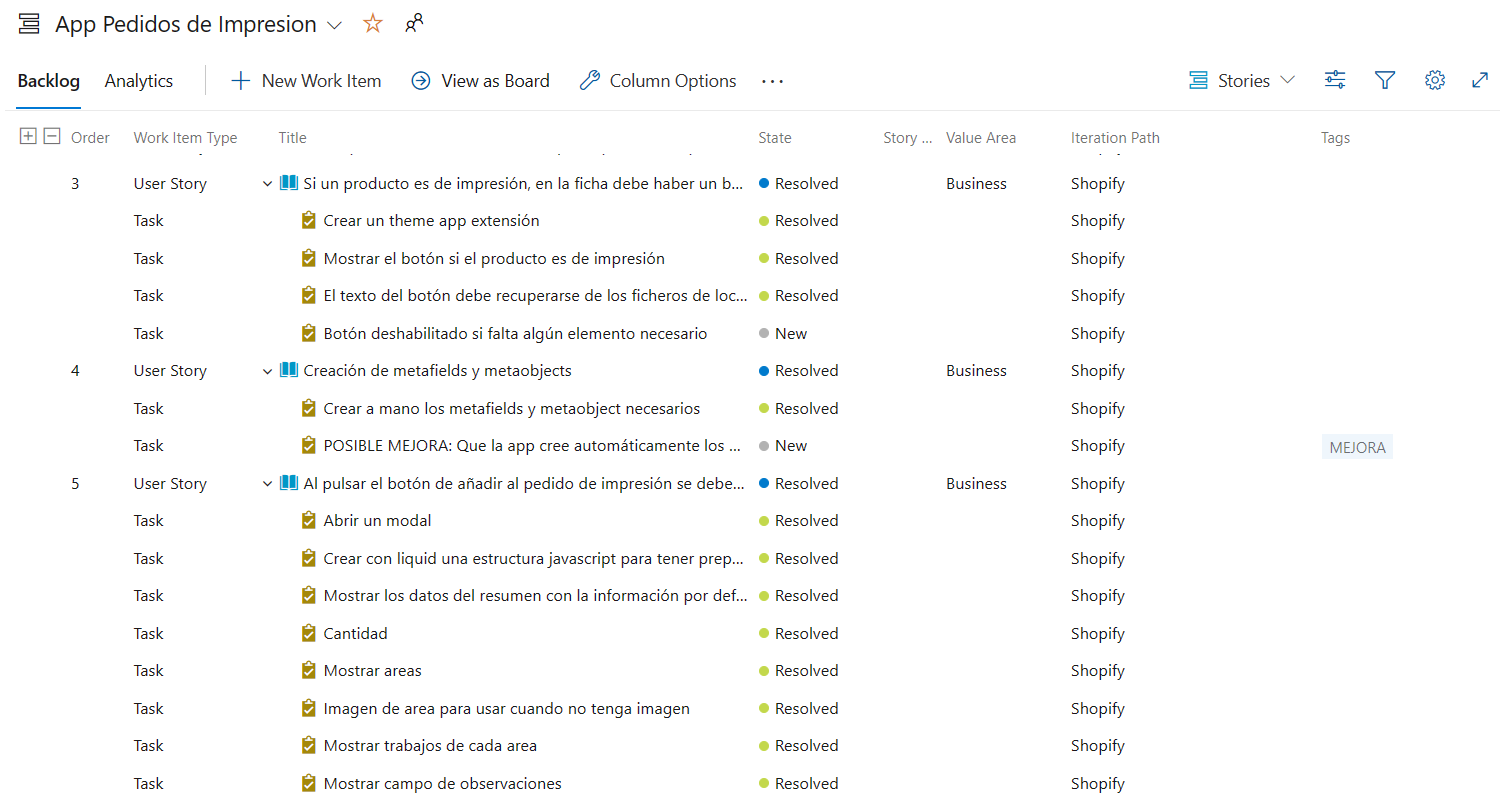
\includegraphics[width=0.8\textwidth]{imagenes/Backlogs de Devops.png}
    \caption{\label{fig:3}Backlogs del proyecto en Azure DevOps}
    \vspace{\fill}
\end{figure}

\begin{figure}[ht]
    \floatplacement{figure}{!t}
    \centering
    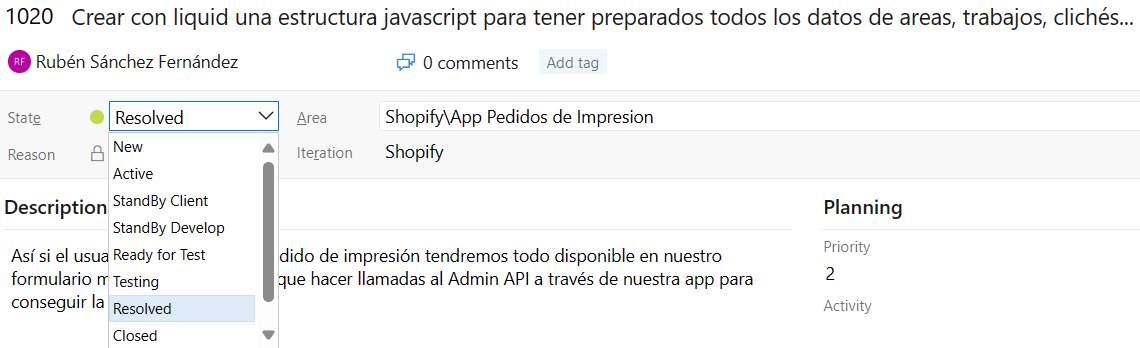
\includegraphics[width=0.8\textwidth]{imagenes/Estados y prioridad de tarea.png}
    \caption{\label{fig:4}Estados y prioridad de una tarea del Backlog}
    \vspace{\fill}
\end{figure}


\clearpage
\section{Diseño y resolución del trabajo realizado}

\subsection{Análisis}
El análisis de este proyecto se ha centrado en la creación de historias de usuario, estas son narrativas 
concisas que describen la funcionalidad deseada desde la perspectiva del usuario final. 
Estas historias de usuario han servido como guía para entender las necesidades de los usuarios y traducirlas en 
funcionalidades concretas que  la aplicación debe proporcionar. Se ha hecho uso de ellas para crear
las tareas que se han ido siguiendo para implementar esta aplicación.

Cada historia de usuario está compuesta por una descripción detallada de la funcionalidad requerida, así como por criterios de aceptación que 
permiten validar que la funcionalidad ha sido implementada de manera adecuada. Estas son la bases sobre las cuales se ha construido y evaluado el éxito de esta aplicación.

\subsubsection{Historias de usuario de las funcionalidades básicas}

\subsubsubsection{Historia de Usuario 1: Botón de Personalizar en la Ficha de Producto}\label{sec:historia1}

Como administrador de la tienda, quiero poder observar en las páginas de producto un botón que posteriormente servirá para activar una funcionalidad de personalización del producto.

\vspace{0.5cm}
\textbf{Criterios de Aceptación:}
\begin{enumerate}[label=\arabic*.]
    \item Cuando visualizo la ficha de un producto en la tienda,
          \begin{itemize}[label=--]
              \item Debe haber un botón claramente identificable como ``Personalizar''.    
          \end{itemize}
    \item El botón ``Personalizar'' solo debe mostrarse si el producto es de impresión,
          \begin{itemize}[label=--]
              \item Un producto se considerará de impresión si tiene información específica en su metafield denominado \textit{upng.areas\_impresion}.
          \end{itemize}
    \item El título del botón debe ser recuperado de los archivos de locales,
          \begin{itemize}[label=--]
              \item Se deben preparar traducciones en inglés y español para el texto del botón y cualquier otro texto relevante en la aplicación.
          \end{itemize}
\end{enumerate}


\subsubsubsection{Historia de Usuario 2: Creación de Metafields y Metaobjects para la Gestión de Trabajos de Impresión}\label{sec:historia2}

Como administrador de la tienda,
quiero tener los metafields y metaobjects necesarios para gestionar los trabajos de impresión,
poder personalizar y administrar eficientemente los productos disponibles de la tienda.

\vspace{0.5cm}
\textbf{Criterios de Aceptación:}
\begin{enumerate}[label=\arabic*.]
    \item Deben existir los metafields y metaobjects requeridos para la gestión de trabajos de impresión.
\end{enumerate}


\subsubsubsection{Historia de Usuario 3: Configurar Impresión al Añadir al Pedido}\label{sec:historia3}

Como administrador de la tienda, deseo poder configurar la impresión de productos antes de añadirlos al pedido, para poder personalizarlos según las necesidades de los clientes.

\vspace{0.5cm}
\textbf{Criterios de Aceptación:}
\begin{enumerate}[label=\arabic*.]
    \item Al pulsar el botón de ``Añadir al Pedido de Impresión'', se debe abrir un modal que permita al usuario configurar la impresión del producto.
    \item El modal debe mostrar toda la información relevante sobre la impresión y permitir al usuario ajustar la configuración según sea necesario.
    \item Se debe crear una estructura JavaScript utilizando Liquid para tener preparados todos los datos de áreas, trabajos, clichés, etc., de manera que no sea necesario realizar llamadas adicionales al Admin API para obtener la información.
    \item En el modal, se debe mostrar un resumen claro y detallado de los elementos seleccionados por el usuario, incluyendo el nombre del producto, la cantidad, las áreas seleccionadas, los trabajos en cada área, los clichés, los precios individuales y el importe total.
    \item El usuario debe poder ingresar la cantidad de productos a imprimir, empleando el selector de cantidad por defecto.
    \item Se deben mostrar las áreas de impresión que tenga el producto y de cada área de impresión debe mostrarse una imagen, su nombre y medidas ajustables (ancho y largo) en inputs. Estos inputs deben validar que el valor máximo sea el de la medida del área y el mínimo sea cero.
    \item Se debe mostrar un checkbox junto a cada área para que el usuario pueda seleccionar en cuáles desea imprimir.
    \item Las imágenes de las áreas que no tengan una definida deben mostrar una imagen por defecto, configurable a través del Theme App Extension.
    \item Cada área debe mostrar los trabajos disponibles en un desplegable para que el usuario pueda seleccionar el que desee.
    \item Cada trabajo tiene un número máximo de colores, por lo que al lado del desplegable de trabajos debe aparecer un desplegable de colores para que el usuario elija el número de colores que necesita. Y cada vez que se actualice el trabajo seleccionado deberá refrescarse este desplegable.
    \item Todos los elementos configurables de las areas, como selectores, inputs, checkbox que el usuario no haya seleccionado deberán aparecer como desactivados.
    \item Se debe habilitar un campo de observaciones en cada área donde el usuario pueda agregar las notas pertinentes.
    \item Para cada trabajo, se debe permitir al usuario seleccionar el número de colores y especificar los colores deseados. Para ello según la selección del usuario en el desplegable de colores se deberán añadir tantos selectores de colores como colores se hayan seleccionado en el mismo. Además del selector de colores se añadirán campos de texto libre para que el usuario pueda especificar cada color mediante esta forma.
    \item Se debe incluir la opción de marcar si un cliché es de repetición, afectando al precio final.
    \item Se debe actualizar dinámicamente la información del resumen al seleccionar o deseleccionar áreas, trabajos y colores.
    \item El usuario debe poder adjuntar una imagen que represente el logo a imprimir para cada área de impresión desde el modal de configuración de del producto. Esta imagen debe ser almacenada en el servidor del administrador.
    \item El diseño del modal debe ser responsive para una experiencia óptima en dispositivos móviles.
    \item Los trabajos deben tener precios diferentes para el color principal (la elección de un solo color) y el resto de colores, con posibilidad de emplear variantes del producto trabajo según sea necesario. Cada color extra que se seleccione debe aplicar un valor añadido al precio base del trabajo.
\end{enumerate}


\subsubsubsection{Historia de Usuario 4: Funcionalidad de Añadir al Carrito}\label{sec:historia4}

Como administrador de la tienda,
quiero poder añadir productos al carrito con su configuración y que al añadir estos productos relacionados (productos normales, trabajos y clichés), estos estén agrupados y vinculados de manera que no se puedan borrar o editar por separado,
para mejorar la experiencia de compra y facilitar la gestión de los productos de impresión.

\vspace{0.5cm}
\textbf{Criterios de Aceptación:}
\begin{enumerate}[label=\arabic*.]
    \item Los productos, junto con su configuración completa (productos normales, trabajos y clichés relacionados), deben agregarse correctamente al carrito al seleccionar la opción ``Añadir al Carrito''.
    \item Al añadir productos al carrito, se deben incluir:
          \begin{itemize}
              \item El producto ``normal''.
              \item Los productos ``trabajo'' seleccionados en diferentes áreas, con la variante adecuada según el número de colores seleccionados.
              \item Los productos ``clichés'' asociados al trabajo, con la variante adecuada según si es de repetición o no.
          \end{itemize}
    \item Se debe investigar si el uso de customized bundles es adecuado para agrupar y vincular los productos relacionados en el carrito.
    \item Estos productos tienen que estar agrupados y de forma que no se puedan eliminar o editar por separado.
    \item Toda la información de impresión configurada (medidas, colores, imagen adjunta y observaciones de cada área) debe guardarse al añadir al carrito, para que pueda transferirse al pedido durante el proceso de checkout.
    \item La cantidad de cada producto añadido al carrito debe ser considerada y reflejada correctamente.
\end{enumerate}

\subsubsection{Historias de usuario de las funcionalidades adicionales}

\subsubsubsection{Historia de Usuario 5: Visualización Agrupada de Productos de Impresión en el Carrito}\label{sec:historia5}

Como administrador de la plataforma,
quiero que los paquetes de productos de impresión (customize bundles), se visualicen completamente de forma agrupada en el carrito de la tienda,
para proporcionar una experiencia de compra clara y comprensible para los clientes.

\vspace{0.5cm}
\textbf{Criterios de Aceptación:}
\begin{enumerate}[label=\arabic*.]
    \item Los productos de impresión deben aparecer agrupados en el carrito, mostrando claramente sus trabajos y clichés asociados.
    \item El detalle de estos paquetes de productos de impresión en el carrito debe ser similar a la visualización que se presenta durante el proceso de checkout.
    \item La visualización agrupada en el carrito debe ser coherente con el diseño y la funcionalidad general de la tienda.
\end{enumerate}


\subsubsubsection{Historia de Usuario 6: Visualización Atractiva del Logo del Cliente en el Producto}\label{sec:historia6}

Como administrador de la tienda,
quiero poder mostrar al cliente una representación visual atractiva de cómo quedaría su logo en el producto,
para ofrecer una experiencia de compra más personalizada y satisfactoria.

\vspace{0.5cm}
\textbf{Criterios de Aceptación:}
\begin{enumerate}[label=\arabic*.]
    \item Se debe poder mostrar una imagen del logo del cliente en el producto de forma atractiva y realista.
    \item La visualización del logo debe reflejar fielmente su posición y tamaño en relación con las áreas designadas del producto.
    \item La implementación de la visualización del logo debe ser viable y práctica dentro del contexto de la tienda en línea.
\end{enumerate}


\subsubsubsection{Historia de Usuario 7: Automatización de la Creación de Metafields Necesarios y objeto cart-transform}\label{sec:historia7}

Como administrador de la tienda,
quiero unas opciones en el panel de administración de la tienda para crear automáticamente los metafields necesarios para la app y el objeto cart-transform,
para simplificar y agilizar el proceso de configuración al instalar la app en una nueva tienda y evitar posibles errores manuales.

\vspace{0.5cm}
\textbf{Criterios de Aceptación:}
\begin{enumerate}[label=\arabic*.]
    \item Se debe proporcionar una opción en el panel de configuración de la tienda para crear automáticamente los metafields necesarios.
    \item Se debe proporcionar una opción en el panel de configuración de la tienda para crear automáticamente el objeto cart-transform.
    \item La creación de estos elementos debe realizarse de manera controlada y asegurarse de no duplicar campos ya existentes.
    \item Después de ejecutar la creación de metafields y el cart-transform, se debe mostrar un mensaje de feedback al usuario indicando el resultado de la operación.
    \item La configuración de los metafields que se crearán debe ser configurable para facilitar la expansión y reutilización de la funcionalidad en otras aplicaciones.
\end{enumerate}


\subsubsubsection{Historia de Usuario 8: Gestión de Casuística ``Doble Pasada'' en Productos y Trabajos}\label{sec:historia8}

Como administrador de la tienda,
quiero poder gestionar la casuística de ``doble pasada'' en productos y trabajos,
para aplicar recargos adicionales en caso de que tanto el producto como el trabajo seleccionados tengan la opción de ``doble pasada'' activada.

\vspace{0.5cm}
\textbf{Criterios de Aceptación:}
\begin{enumerate}[label=\arabic*.]
    \item Debe existir un nuevo metafield booleano llamado ``DOBLE PASADA'' para los productos y los trabajos.
    \item Si se selecciona un producto con la opción ``DOBLE PASADA'' activada y se elige un trabajo que también tenga esta opción activada, se debe mostrar en el presupuestador un check para permitir al usuario seleccionar la opción de ``doble pasada''.
    \item Si se cambia el trabajo seleccionado a uno que no tenga la opción de ``doble pasada'', el check debe ocultarse automáticamente.
    \item Este recargo adicional debe mostrarse en el resumen del pedido del presupuestador y aplicarse al pedido debidamente.
\end{enumerate}


\subsubsubsection{Historia de Usuario 9: Gestión del Canon Digital y Adición Automática al Carrito}\label{sec:historia9}

Como administrador de la tienda,
quiero poder gestionar el canon digital en ciertos productos,
para aplicar un importe fijo adicional al precio de algunos productos específicos.

\vspace{0.5cm}
\textbf{Criterios de Aceptación:}
\begin{enumerate}[label=\arabic*.]
    \item Debe existir un metafield llamado ``Importe Canon'' para los productos, que permita indicar si un producto tiene canon digital y especificar el importe correspondiente.
    \item Se debe crear un producto especial con un precio de un céntimo, que se utilizará para añadir el importe del canon digital al carrito de compra.
    \item Cuando se añada un producto al carrito, se debe agregar automáticamente una línea de canon digital asociada al producto (ya sea un producto normal o uno personalizado).
    \item La línea de canon digital debe estar vinculada al producto correspondiente y reflejar el importe del canon establecido para ese producto.
    \item Se deben utilizar customize bundles para asociar cada línea de producto con su línea de canon digital correspondiente en el carrito.
\end{enumerate}

\subsection{Diseño}
En el desarrollo de este Trabajo de Fin de Grado, el diseño de la aplicación ha sido una parte fundamental que ha sentado las bases para la implementación
de las funcionalidades requeridas. Este diseño se ha basado en un minucioso estudio de las tecnologías pertinentes, así como en la comprensión detallada de las
historias de usuario que definían los objetivos y requisitos del proyecto. Este diseño se ha estructurado en torno a la definición de diversas tareas que han sido cuidadosamente 
elaboradas.

Estas tareas de diseño abarcan desde la creación de la estructura inicial de la aplicación, hasta la implementación de características específicas que 
garantizan una experiencia fluida y eficiente para los usuarios finales. Se han tenido en consideración, tanto las necesidades básicas de funcionamiento, como aquellas funcionalidades
adicionales que agregan más valor al sistema.

Es importante destacar, que en este apartado las tareas de diseño se dividen en dos categorías: las tareas básicas, que se centran en la implementación de la funcionalidad
principal de la aplicación y en conseguir cumplir con éxito los criterios de aceptación de las historias de usuario de funcionalidad básica. Y las tareas adicionales, que 
añaden una funcionalidad y complejidad adicional, y se centran en cumplir los criterios de aceptación de las historias de usuario de la funcionalidad adicional.


\subsubsection{Tareas básicas}

\textbf{Tareas relacionadas con la \hyperref[sec:historia1]{Historia de usuario 1}:}
\begin{itemize}
    \item \textbf{Tarea 1:} Crear una Aplicación y una Extensión de Tema:
          \begin{itemize}[label=--]
              \item \textbf{Descripción:} Crear una aplicación para Shopify con el template Node e instalarla en la tienda. Crear un theme app extensión en la aplicación para poder añadir una nueva sección con el botón y toda su funcionalidad a las plantillas de ficha de producto a través del personalizador del theme en la tienda.
          \end{itemize}
    \item \textbf{Tarea 2:} Crear la sección con el botón y mostrarlo solo si el Producto es de Impresión:
          \begin{itemize}[label=--]
              \item \textbf{Descripción:} Crear una sección en el theme app extension y añadir en ella un botón. Utilizar liquid para verificar si el producto de la página en la que se ejecute es de impresión. Un producto se considerará de impresión si tiene información específica en su metafield denominado \textit{upng.areas\_impresion}.
              \item Mostrar el botón ``Personalizar'' si el producto cumple con los criterios establecidos; de lo contrario, ocultar el botón.
          \end{itemize}
    \item \textbf{Tarea 3:} Recuperar el Texto del Botón de los Archivos de Locales:
          \begin{itemize}[label=--]
              \item \textbf{Descripción:} Configurar la aplicación para que el texto del botón y cualquier otro texto relacionado se recupere de los archivos de locales. Preparar traducciones en inglés y español para garantizar una experiencia multilingüe completa.
          \end{itemize}
\end{itemize}

\textbf{Tareas relacionadas con la \hyperref[sec:historia2]{Historia de usuario 2}:}
\begin{itemize}
    \item \textbf{Tarea 1:} Crear Manualmente los Metafields y Metaobjects Necesarios:
          \begin{itemize}[label=--]
              \item \textbf{Descripción:} Crear manualmente los metafields y metaobjects necesarios para la gestión de trabajos de impresión. Habrá que crear un metaobjeto area de impresión, que contenga todos los atributos necesarios que se van a necesitar (nombre, imagen, alto, ancho y trabajos). Se crearán metacampos para la entidad producto que contengan una lista de metaobjetos del tipo area de impresión, el número de colores para los productos de tipo trabajo y una metacampo que sea una referencia al cliche (producto especial).
          \end{itemize}
\end{itemize}

\textbf{Tareas relacionadas con la \hyperref[sec:historia3]{Historia de usuario 3}:}
\begin{itemize}
    \item \textbf{Tarea 1:} Abrir un modal:
          \begin{itemize}[label=--]
              \item \textbf{Descripción:} Al pulsar el botón ``Añadir al Pedido de Impresión'', se debe abrir un modal que contenga toda la información necesaria para configurar la impresión del producto.
          \end{itemize}
    \item \textbf{Tarea 2:} Crear estructura JavaScript para datos de impresión:
          \begin{itemize}[label=--]
              \item \textbf{Descripción:} Utilizar Liquid para crear una estructura JavaScript que contenga todos los datos relevantes de áreas, trabajos, clichés, etc., necesarios para la configuración de la impresión. Esto permitirá tener los datos disponibles en el modal sin necesidad de realizar llamadas adicionales al Admin API.
          \end{itemize}
    \item \textbf{Tarea 3:} Mostrar datos del resumen:
          \begin{itemize}[label=--]
              \item \textbf{Descripción:} En el modal, mostrar una sección de resumen que presente de manera clara y detallada todos los elementos seleccionados por el usuario, incluyendo el nombre del producto, cantidad, áreas seleccionadas con sus trabajos y clichés asociados, precios individuales y el importe total. Esta sección debe actualizarse dinámicamente al configurar diferentes elementos de la impresión.
          \end{itemize}
    \item \textbf{Tarea 4:} Ajustar la cantidad de productos:
          \begin{itemize}[label=--]
              \item \textbf{Descripción:} Se pueden configurar a la vez tantas unidades de producto como se quieran. En principio se compartira el mismo input de cantidad ya existente en la ficha del producto. Al ingresar un número de unidades en la ficha de producto y pulsar el botón del configurador, se tendrá en cuenta el valor de dicho input para establecer el número de productos a configurar. Se hará uso del valor del mismo a la hora de hacer los cálculos del resumen y añadir los elementos necesarios al carrito.
          \end{itemize}
    \item \textbf{Tarea 5:} Mostrar áreas de impresión:
          \begin{itemize}[label=--]
              \item \textbf{Descripción:} Mostrar todas las áreas de impresión disponibles para el producto, incluyendo todos sus elementos imagen, nombre y medidas ajustables (ancho y largo). Estos datos se obtendran del la estructura javascript que se habrá preparado con todos los datos del prodcuto actual y estarán disponibles en el modal. Se habilitará un checkbox junto a cada nombre para que el usuario pueda seleccionar las áreas en las que desea imprimir.
          \end{itemize}
    \item \textbf{Tarea 6:} Imagen por defecto para áreas sin imagen:
          \begin{itemize}[label=--]
              \item \textbf{Descripción:} Configurar una imagen por defecto para las áreas que no tengan una imagen definida. Para ello en el Schema de la configuración de la sección, se añadira una settings de imagen, para que el administrador de la tienda pueda escoger esta imagen desde el panel de administración del tema. En los assets de la aplicación se incluirá otra imagen de reserva por si el administrador no hubiera configurado esta opción. A la hora de mostrar las areas se comprobará si tienen o no imagen, en caso negativo se empleará la configurada en esta setting y como último recurso la almacenada en assets.
          \end{itemize}
    \item \textbf{Tarea 7:} Mostrar trabajos para cada área y número de colores del trabajo:
          \begin{itemize}[label=--]
              \item \textbf{Descripción:} En cada área, se debe presentar un desplegable con los trabajos disponibles para que el cliente pueda elegir el deseado. Cada trabajo tiene un número máximo de colores. Junto al desplegable de trabajos, se mostrará un desplegable de colores para que el usuario seleccione el número necesario de colores con el que quiere realizar el trabajo de impresión. Al cambiar el trabajo seleccionado, se actualizarán dinámicamente las opciones disponibles en el desplegable de colores, pues cada trabajo cuenta con un límite de colores. Al seleccionar un trabajo para un área específica, se actualizará automáticamente la información del resumen con su nombre y precio correspondiente. El precio del trabajo será calculado multiplicando el precio del trabajo por el número de productos que se están personalizando, pues a cada unidad hay que aplicarle un trabajo.
          \end{itemize}
    \item \textbf{Tarea 8:} Incluir campo de observaciones:
          \begin{itemize}[label=--]
              \item \textbf{Descripción:} En cada área de impresión, incluir un campo de observaciones donde el usuario pueda agregar notas pertinentes relacionadas con la impresión.
          \end{itemize}
    
    \item \textbf{Tarea 9:} Marcar cliché de repetición:
          \begin{itemize}[label=--]
              \item \textbf{Descripción:} En cada area, debe aparecer un checkbox para que el usuario pueda indicar si el cliché es de repetición (no es la primera vez que se hace una impresión con la imagen que desea el cliente) o no. Este factor afectará al precio final de la impresión. El cliche será un producto especial que contará con dos variantes, una con su precio normal (variante: NO) y otra con un precio más económico (variante: SI) correspondiente a la repetición de cliche. En caso de marcar este checkbox se tendrá en cuenta la variante de repetición y en caso contrario su variante normal, aplicando de este modo un precio u otro al pedido. Además, hay que tener en cuenta que en un área de impresión configurada, se añadiran tantos cliches al pedido de personalización como colores haya seleccionado el usuario. Esto se debe a que el proveedor de la tienda deberá fabricar un cliche por cada color en el que se desee imprimir, por lo que el cliente debe acarrear con su coste.
          \end{itemize}
    \item \textbf{Tarea 10:} Seleccionar áreas:
          \begin{itemize}[label=--]
              \item \textbf{Descripción:} Cuando se marque un area se deben habilitar y deshabilitar todos los elementos configurables de la misma (campos de trabajos, colores, medidas, etc.). Se debe actualizar la información del resumen con los elementos y precios correspondientes, sumando los precios del trabajo seleccionado, colores, cliche y demás elementos. En caso de que se desmarque la opción no se tendrán en cuenta los elementos y configuracions de esta area y no aparecerá en el resumen.
          \end{itemize}
    \item \textbf{Tarea 11:} Mostrar selectores de colores:
          \begin{itemize}[label=--]
              \item \textbf{Descripción:} Al seleccionar un número de colores en el desplegable, se debe añadir un campo de texto por cada uno de estos colores, para que el usuario pueda indicar en que color se debe imprimir. Este será un campo de texto libre. Además se ofrecerá un selector para que el usuario pueda escoger entre varios colores. Actualizar la cantidad de clichés y multiplicar su precio en el resumen.
          \end{itemize}
    \item \textbf{Tarea 12:} Adjuntar imagen por área:
          \begin{itemize}[label=--]
              \item \textbf{Descripción:} Para cada area, se mostrará un campo para poder adjuntar una imagen. Se deberá crear un método de API en nuestra aplicación, para que el usuario pueda subir la imagen realizando una llamada a la misma y almacenando la imagen en el servidor del administrador. Se deberá nombrar a la imagen en el servidor con un nombre que nos permita identificarla y asociarla al area del pedido del cliente. Para ello se generará un identificador aleatorio que se asociará al producto de impresión y que deberá almacenarse junto con el resto de datos de impresión que se configuran. Se empleará este identificador como parte del nombre de la imagen. Para mejor clasificación se puede crear una subcarpeta con la fecha actual en el directorio de imagenes del servidor, de este modo se realizará un almacenamiento de las imagenes más ordenado de cara al administrador de la tienda.
          \end{itemize}
    \item \textbf{Tarea 13:} Diseño responsive:
          \begin{itemize}[label=--]
              \item \textbf{Descripción:} Asegurar que el diseño del modal y la forma de mostrar los elementos sea óptima y clara en la vista móvil.
          \end{itemize}
    \item \textbf{Tarea 14:} Precios diferenciados para trabajos según colores:
          \begin{itemize}[label=--]
              \item \textbf{Descripción:} En este tipo de pedidos de impresión, los trabajos serán productos especiales que han de tener dos variantes con dos precios distintos. Habrá una variante ``Primer color'' y otra variante ``Resto colores''. Si el usuario selecciona un color en el area, se le cobrará un trabajo principal, pero si ha seleccionado más de un color, se le cobrará el primero como trabajo principal y el resto con el precio del trabajo secundario, que es más económico pero representa un coste adicional de trabajo al tener que imprimir en varios colores. Es decir se deberá añadir una variante de trabajo de resto colores por cada color adicional.
          \end{itemize}
\end{itemize}

\textbf{Tareas relacionadas con la \hyperref[sec:historia4]{Historia de usuario 4}:}
\begin{itemize}
    \item \textbf{Tarea 1:} Añadir Productos Relacionados al Carrito:
          \begin{itemize}[label=--]
              \item \textbf{Descripción:} Implementar la lógica para añadir al carrito los productos relacionados, incluyendo el producto ``normal'', los ``trabajos'' seleccionados en las diferentes areas con la variante adecuada según el número de colores seleccionados y los ``clichés'' asociados, teniendo en cuenta las cantidades según las selecciones del usuario. Investigar y utilizar el ajax API para añadir todos los elementos al carrito.
          \end{itemize}
    \item \textbf{Tarea 2:} Guardar Información de Impresión en el Carrito:
          \begin{itemize}[label=--]
              \item \textbf{Descripción:} Desarrollar la funcionalidad para guardar toda la información de impresión configurada (medidas, colores, identificador de la imagen adjunta, observaciones de cada área y todos los atributos necesarios) en el carrito al añadir productos relacionados. Estos datos deben almacenarse junto con el pedido de impresión realizado y estar disponibles en el checkout y el pedido final que se recibirá en el panel de administración de la tienda. Para ello una buena opción es usar las propiedades de líneas de pedido \cite{properties-lineitem} que proporciona Shopify para almacenar atributos de un producto en el carrito.
          \end{itemize}
    \item \textbf{Tarea 3:} Investigar el Uso de Customized Bundles para Agrupar y Vincular Productos:
          \begin{itemize}[label=--]
              \item \textbf{Descripción:} Investigar si los \textbf{customized bundles} \cite{paquete-personalizado} son una solución adecuada para agrupar y vincular los productos relacionados en el carrito de manera que no se puedan borrar o editar por separado. Analizar visualmente cómo se mostrarían en el carrito, el checkout y en el historial de pedidos. Si no se considera viable el uso de customized bundles, explorar la posibilidad de utilizar JavaScript para agregar esta funcionalidad al carrito, especialmente enfocado en impedir cambios individuales en los productos relacionados.
          \end{itemize} 
\end{itemize}

\subsubsection{Tareas adicionales}

\textbf{Tareas relacionadas con la \hyperref[sec:historia5]{Historia de usuario 5}:}
\begin{itemize}
    \item \textbf{Tarea 1:} Modificar el Theme para Mostrar el Detalle de los Bundles de Impresión en el Carrito:
          \begin{itemize}[label=--]
              \item \textbf{Descripción:} Como se ha podido observar, los paquetes de productos de personalización que se muestran en el carrito (customized bundles), no muestran los detalles de los artículos que contienen con sus precios. Estos paquetes se muestran como un solo artículo de tipo paquete cuyo contenido no se puede visualizar. El objetivo de esta tarea es desarrollar una sección en el tema de una tienda estandar, que sea una versión de la sección \texttt{main-cart-items.liquid} (sección en la que se muestran los productos del carrito) en la que se muestre el detalle de estos paquetes de impresión de manera similar a la visualización en el proceso de checkout.
          \end{itemize}
\end{itemize}


\textbf{Tareas relacionadas con la \hyperref[sec:historia6]{Historia de usuario 6}:}
\begin{itemize}
    \item \textbf{Tarea 1:} Investigar Opciones para Mostrar el Logo del Cliente en la Zona Adecuada del Producto e implementarlo:
          \begin{itemize}[label=--]
              \item \textbf{Descripción:} Realizar una investigación exhaustiva para identificar opciones, librerías u herramientas que permitan mostrar la imagen del logo que adjunta el cliente para cada area en el personalizador de productos. Esta imagen se debe mostrar en la zona adecuada del producto de una forma atractiva y en la posición adecuada. Evaluar la viabilidad de cada opción en función de la información disponible sobre el producto de impresión y las necesidades específicas del cliente. Por último, implementar la solución elegida.
          \end{itemize}
\end{itemize}

\textbf{Tareas relacionadas con la \hyperref[sec:historia7]{Historia de usuario 7}:}
\begin{itemize}
    \item \textbf{Tarea 1:} Limpiar la Interfaz del Administrador de la App:
          \begin{itemize}[label=--]
              \item \textbf{Descripción:} Eliminar las opciones demo y botones relacionados en la parte frontal de la interfaz de administración de la app para eliminar funcionalidad innecesaria (al crear la app con el template Node, este viene con una funcionalidad de ejemplo en la interfaz de administración de la app).
          \end{itemize}
    \item \textbf{Tarea 2:} Agregar un Botón ``Crear Metacampos Necesarios'' y otro ``Crear objeto cart-transform'' en la Interfaz de Administración :
          \begin{itemize}[label=--]
              \item \textbf{Descripción:} Incorporar un botón en la interfaz de administración por cada acción que se desea realizar. Uno para activar la creación de metadatos y otro para activar la creación del objeto cart-transform. Cada botón llamará al método de la app correspondiente para crear los elementos adecuados.
          \end{itemize}
    \item \textbf{Tarea 3:} Desarrollar el Endpoint y el Método para Crear los Metafields Necesarios y asociarlo al botón correspondiente:
          \begin{itemize}[label=--]
              \item \textbf{Descripción:} Crear un endpoint y un método en la app al que llame, que utilice llamadas al API de GraphQL para crear los metafields y los metaobject necesarios, controlando si ya existen. Además realizar la llamada correspondiente desde la parte del frontend para que al pulsar el botón se llame al método creado y se ejecute la acción pertinente.
          \end{itemize}
    \item \textbf{Tarea 4:} Desarrollar el Endpoint y el Método para Crear el objeto cart-transform y asociarlo al botón correspondiente:
          \begin{itemize}[label=--]
              \item \textbf{Descripción:} Crear un endpoint y un método en la app al que llame, que utilice llamadas al API de GraphQL para crear el objeto cart-transform, controlando si ya existe. Además realizar la llamada correspondiente desde la parte del frontend para que al pulsar el botón se llame al método creado y se ejecute la acción pertinente.
          \end{itemize}
    \item \textbf{Tarea 5:} Implementar la Funcionalidad de Feedback para el Usuario:
          \begin{itemize}[label=--]
              \item \textbf{Descripción:} Desarrollar una funcionalidad en la interfaz de administración de la app para mostrar un mensaje de feedback al usuario después de la ejecución de los métodos implementados, informando sobre el éxito o posibles errores.
          \end{itemize}
    \item \textbf{Tarea 6:} Hacer Configurable la Creación de Metafields:
          \begin{itemize}[label=--]
              \item \textbf{Descripción:} Crear un fichero de configuración o constantes que definan los metafields que se crearán, para qué entidad y de qué tipo. Adaptar el código para usar esta configuración, permitiendo así una fácil expansión y reutilización de la funcionalidad en otras aplicaciones.
          \end{itemize}
\end{itemize}

\textbf{Tareas relacionadas con la \hyperref[sec:historia8]{Historia de usuario 8}:}
\begin{itemize}
    \item \textbf{Tarea 1:} Crear Metafields para ``Doble Pasada'' en Productos:
          \begin{itemize}[label=--]
              \item \textbf{Descripción:} Utilizar la funcionalidad de creación automática de metafields para crear un metafield booleano llamado ``DOBLE PASADA'' para los productos.
          \end{itemize}
    \item \textbf{Tarea 2:} Mostrar el Check para ``Doble Pasada'':
          \begin{itemize}[label=--]
              \item \textbf{Descripción:} Implementar la lógica para mostrar un check junto al trabajo seleccionado en el presupuestador si tanto el producto como el trabajo tienen la opción de ``doble pasada'' activada. Asegurarse de que el check se oculte automáticamente si se cambia el trabajo seleccionado a uno que no tenga la opción de ``doble pasada''.
          \end{itemize}
    \item \textbf{Tarea 3:} Aplicar cargo extra de ``Doble Pasada'':
          \begin{itemize}[label=--]
              \item \textbf{Descripción:} Si el usuario marca el check de doble pasada, se deberá aplicar al pedido, un cargo por doble pasada equivalente a añadir un color más (añadir una variante ``Resto colores'' del tabajo al pedido). En el resumen de impresión debe mostrarse este concepto y el importe añadido correspondiente. Además al añadir este cargo al carrito, se debe reflejar de algún modo que esta variante de trabajo añadida corresponde a este tipo de cargo adicional, para ello sería conveniente usar las propiedades de la API de carrito de Shopify.
          \end{itemize}
\end{itemize}

\textbf{Tareas relacionadas con la \hyperref[sec:historia9]{Historia de usuario 9}:}
\begin{itemize}
    \item \textbf{Tarea 1:} Crear Metafield para el Importe del Canon Digital:
          \begin{itemize}[label=--]
              \item \textbf{Descripción:} Crear un metafield de tipo número decimal, llamado ``Importe Canon'', utilizando la funcionalidad de creación automática de metafields. Este metafield se usará para indicar si un producto tiene canon digital y especificar el importe correspondiente. Los productos sin canon no tendrán nada en este metacampo, y los productos con canon tendrán en este metacampo el importe correspondiente.
          \end{itemize}
    \item \textbf{Tarea 2:} Crear Producto Especial para Añadir el Importe al Carrito:
          \begin{itemize}[label=--]
              \item \textbf{Descripción:} Crear un producto especial con un precio de un céntimo, que se utilizará únicamente para añadir el importe del canon digital al carrito de compra. Este producto especial asegurará que el importe del canon se aplique correctamente al total del carrito de compra.
          \end{itemize}
    \item \textbf{Tarea 3:} Añadir Líneas de Canon al Carrito y Asociarlas a sus Productos Correspondientes con customize bundles:
          \begin{itemize}[label=--]
              \item \textbf{Descripción:} Cuando se añada un producto con canon al carrito, se deberá añadir una línea de canon digital (producto especial creado) para repercutir el canon.
              Cómo el producto especial tiene un precio de un céntimo, se deberá jugar con la cantidad de este artículo para conseguir obtener el importe del canon de producto al que se le está aplicando. Por ejemplo
              si un producto tiene 1,20€ de canon digital, se añadirá el producto especial con cantidad 120.
              Este canon digital se deberá añadir tanto a los productos ``normales'' que no sean de impresión, como a los productos de impresión.
              Para los productos que sean de impresión se deberá realizar una configuración adicional en el procedimiento de adición con la API de AJAX, para que en caso de que el producto personalizado cuente con canon digital, se añada la cantidad adecuada de productos canon de un céntimo y se agrupe con el resto de artículos del paquete de impresión en el carrito.
              Para los productos normales, se debe investigar si modificando la funcionalidad de los cart-tranform existente (customize bundles), se pueden extender los productos ``normales'' que cuenten con canon digital y que en el carrito, se cree automáticamente un paquete con cada producto normal y su canon asociado, con la cantidad adecuada.
          \end{itemize}
\end{itemize}


\subsection{Implementación}
La implementación de esta aplicación, se ha llevado a cabo siguiendo una guía estructurada en base a las tareas definidas durante la fase de diseño.
Es importante remarcar que el proceso de implementación siguió una metodología iterativa e incremental como ya se ha comentado. Inicialmente, se llevó a cabo el desarrollo
de las historias de usuario y el diseño detallado de las tareas en base a dichas historias, centrándose unicamente en las funcionalidades básicas. Se priorizó
la implementación de estas tareas, las cuales abordaban los requisitos esenciales de la aplicación. Una vez que se obtuvo la primera implementación del
proyecto básico, se procedió a analizar, desarrollar e implementar las tareas adicionales. Este enfoque iterativo e incremental permitió una implementación
ordenada y eficiente, garantizando que cada fase del desarrollo se construyera sobre una base sólida y que se respondiera de manera ágil a los cambios y mejoras.

En esta sección, se presentará la implementación dividida en cuatro partes: la creación de la aplicación y la extensión de tema, el desarrollod el backend, la elaboración del frontend de la parte de administración y una última sección donde se detallará el empleo de los customize boundles y las modificaciones realizadas en un tema estandar de la tienda. Esta división 
proporciona una visión clara y organizada de la implementación del proyecto.

\subsubsection{Creación de la aplicación e implementación del theme app extension}
Para empezar con este desarrollo, cabe destacar que de partida se cuenta con una tienda de desarrollo de Shopify Plus que constituye un entorno de pruebas con datos ficticios.
Este entorno de trabajo sería similar a una tienda real de un cliente que podía solicitar los servicios de la aplicación a desarrollar, por lo que todos las modificaciones e implementaciones
que se lleven a cabo en la tienda, serán un ejemplo de las modificaciones y adaptaciones que se deberán hacer en una tienda real a la hora de adaptarla para instalar la aplicación final.

En primer lugar antes de comenzar con la implementación de la aplicación, se crean en la tienda de desarrollo los metafields y metaobjetos necesarios para gestionar
los trabajos de impresión. Para ello se debe acceder a la pantalla de configuración del panel de administración de la tienda. En la Figura~\ref{fig:configuracionMetafields} se puede ver
esta pantalla de configuración, en la que se debe acceder a la sección de ``Datos personalizados''. En este apartado se pueden crear de forma manual,
tanto definiciones de metaobjetos como de metacampos.

\begin{figure}[ht]
    \floatplacement{figure}{!t}
    \centering
    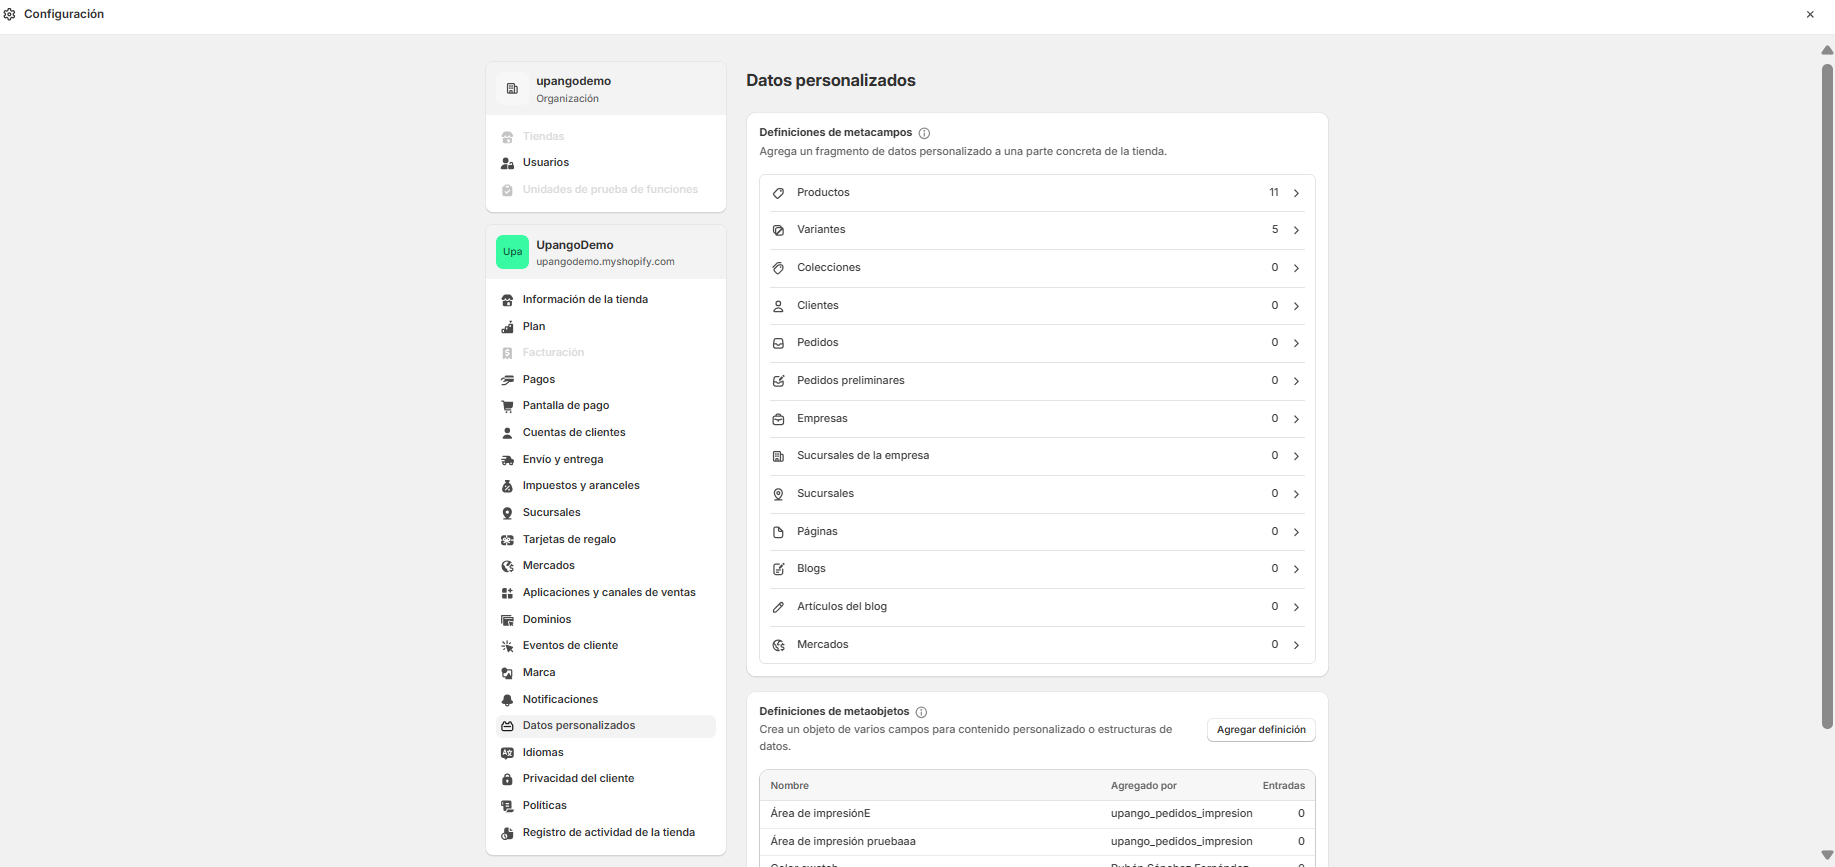
\includegraphics[width=0.8\textwidth]{imagenesUS2/configuracionAdministradorTienda.png}
    \caption{\label{fig:configuracionMetafields}Pantalla de configuración de la interfaz de administración de la tienda}
    \vspace{\fill}
\end{figure}

Los productos personalizables de las tiendas, deberán contar con sus correspondientes áreas de impresión, estas representan
las zonas del producto donde se puede realizar una personalización y cuentan con información relevante sobre dicha zona.
Para representar estas áreas se debe crear un metaobjeto de ``Área de impresión''. En la Figura~\ref{fig:metaobjeto} se puede ver la estructura de este 
objeto. Este cuenta con un nombre del área, la imagen que respresenta la zona del producto a personalizar, el alto y ancho máximo que puede tener la impresión y 
los trabajos de impresión asociados al área (lista de referencias de producto). 

Los trabajos son los diferentes tipos de impresión que se pueden aplicar a un área de un producto, por ejemplo, impresión láser, serigrafía, entre otros.
Estos trabajos se van a representar en la tienda como productos especiales con su precio correspondiente. Estos estarán configurados de tal forma que no sean accesibles a través de la tienda, y
no se puedan comprar por separado, no permitirá rastrear su cantidad, por lo que no tendrán stock y tampoco requeriran de envío.

Otro tipo de productos especiales que deberán existir en las tiendas son los clichés. Estos hacen referencia a las planchas tipográficas donde se reproduce una composición o grabado
a imprimir. Este tipo de productos tampoco será visible ni se permitirá comprar por separado en la web de la tienda y tampoco permitirá envío  ni tendrá stock.
Además este contará con dos variantes ``SI'' y ``NO'' para indicar si el cliché es de repetición o no (esta funcionalidad se especificará mas adelante).


\begin{figure}[ht]
    \floatplacement{figure}{!t}
    \centering
    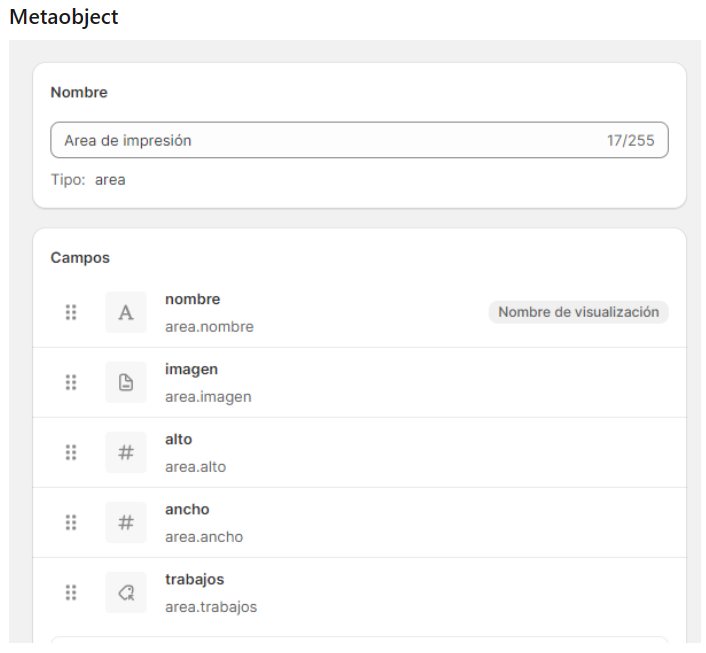
\includegraphics[width=0.8\textwidth]{imagenesUS2/creacionMetaobjeto.png}
    \caption{\label{fig:metaobjeto}Estructura del metaobjeto}
    \vspace{\fill}
\end{figure}

En cada trabajo de impresión se hace uso de un cliché determinado, por lo que cada trabajo debe tener asociado su producto cliché correspondiente. Por ello se debe 
crear la definición del metacampo ``Cliché del trabajo'', para el tipo de elemento ``Producto''. Esta definición será del tipo ``referencia de produto''. De esta forma al crear los productos trabajos correspondientes se le podrá asociar su producto cliché vinculado.

Además cada trabajo también cuenta con un número de colores que permite, por lo que se deberá crear también una definición de metadato ``Número de colores para trabajo'' que permita
introducir el número de colores que permite cada trabajo de la tienda.

Por último como se ha comentado, cada producto normal de la tienda debe contar con sus correspondientes áreas de impresión, por lo que se debe crear otro metadato para el tipo de elemento ``Producto''. Este será una 
lista del metaobjeto que se ha configurado (``Áreas de impresión''). En la Figura~\ref{fig:metadatos} se pueden observar las definiciones los 3 tipos de metadatos configurados para los productos.

\begin{figure}[ht]
    \floatplacement{figure}{!t}
    \centering
    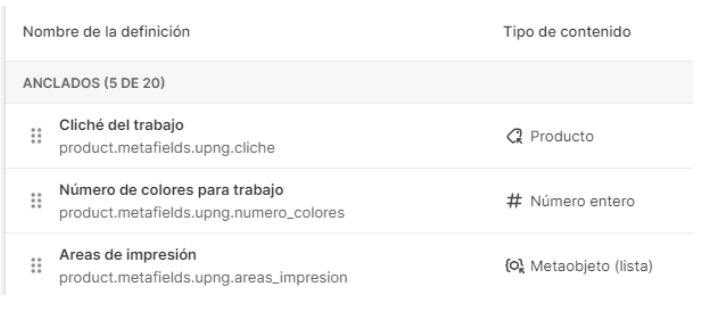
\includegraphics[width=0.8\textwidth]{imagenesUS2/creacionMetafields.png}
    \caption{\label{fig:metadatos}Estructura de los metadatos}
    \vspace{\fill}
\end{figure}

Una vez configurados los elementos necesarios en la tienda, se procede a crear la aplicación. Para ello se ha hecho uso de la Shopify CLI \cite{shopify-cli}, esta herramienta
de línea de comandos proporciona mecanismos para automatizar la generación de una aplicación para Shopify, además de muchas otras funcionalidades.
Para generar la aplicación se ejecuta el siguiente comando desde el directorio en el que se desee almacenar la aplicación: 
\begin{lstlisting}
    npm init @shopify/app@latest -- --template=node
\end{lstlisting}

Este comando establece una estructura base sobre la cual comenzar a trabajar. Es importante destacar que se especifica el uso del template de aplicación basada en Node.js 
para la generación del proyecto.

Después de haber creado la aplicación inicial, el siguiente paso es generar una ``theme app extension'' sobre la cual se trabajará la parte visual del tema. Esta
extensión permite la integración de la aplicación (frontend) con el tema de la tienda de Shopify.

Para generar la extensión se vuelve a emplear la Shopify CLI y se introduce el siguiente comando:

\begin{lstlisting}
    shopify app generate extension
\end{lstlisting}

Al ejecutar este comando hay que seleccionar el tipo de extensión que se desea implementar y proporcionar el nombre de la extensión. Una vez completado este proceso,
se generará la estructura inicial de la extensión del tema, proporcionando una base sobre la que poder trabajar y desarrollar la parte del frontend de la aplicación que se integrará con
el tema de la tienda.

Una vez se tiene la aplicación base con su theme app extensión correspondiente, ya se puede empezar a trabajar sobre la extensión para implementar la funcionalidades básicas.

En primer lugar se crea la sección sobre la cual se va a implementar toda la funcionalidad. El contenido de esta sección solo debe ejecutarse y estar disponible en las 
páginas de productos que sean personalizables. En la Figura~\ref{fig:creacionSeccion} se puede ver como se ha creado la sección \textit{botonPersonalizar.liquid}. En ella lo primero
que se hace es recuperar las areas de impresión del producto actual. Una vez se obtienen las areas de impresión, se ejecuta una condición para comprobar
si el producto posee áreas de impresión o no. En caso afirmativo, se ejecutará la funcionalidad de la sección.

En esta sección se ha creado un botón que será el encargado de mostrar un modal con todas las opciones de personalización. Gracias a la comprobación
que se realiza al principio de la sección, este botón junto con la funcionalidad que lleva detrás solo estará disponible en las páginas de productos personalizables.
El texto del botón y todos los textos que se emplean en esta aplicación son obtenidos de los ficheros locales. Estos son archivos de idioma en formato 
JSON que sirven para almacenar las diferentes traducciones. Cada archivo de idioma corresponde a un idioma específico y contiene un conjunto de etiquetas con su valor-traducción correspondiente. Esto nos 
permite preparar traducciones en varios idiomas para garantizar una experiencia multilinüe completa.

En la parte izquierda de la Figura~\ref{fig:locales} se puede observar como en el directorio de locales existen 2 ficheros, uno para el idioma ingles y otro para el español. 
Ambos contienen las mismas etiquetas pero, cada uno posee las traducciones en su idioma. En un futuro si la aplicación necesitase adaptarse a más idiomas, se podrían crear los ficheros locales
necesarios con sus traducciones correspondientes.


\begin{figure}[ht]
    \floatplacement{figure}{!t}
    \centering
    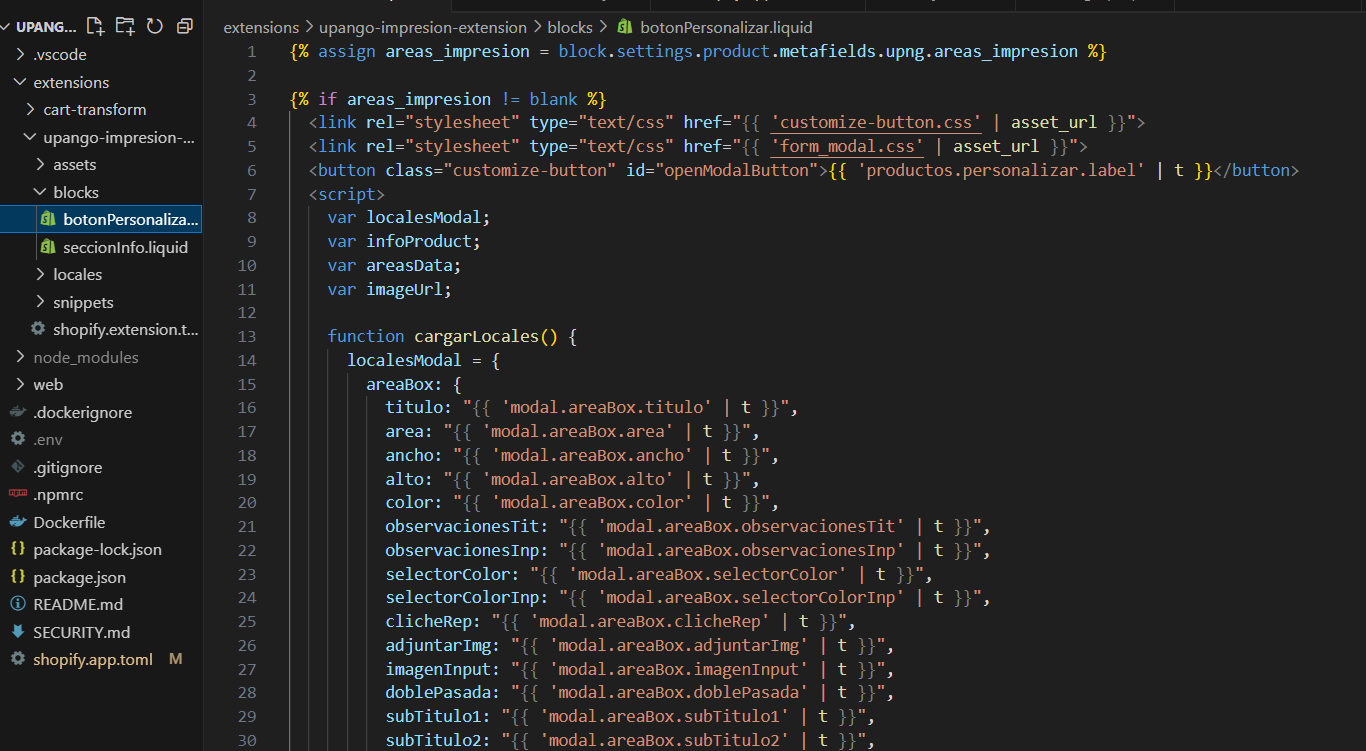
\includegraphics[width=0.8\textwidth]{imagenesUS1/seccionPersonalizarBoton.png}
    \caption{\label{fig:creacionSeccion}Creación de la sección botonPersonalizar.liquid}
    \vspace{\fill}
\end{figure}

\begin{figure}[ht]
    \floatplacement{figure}{!t}
    \centering
    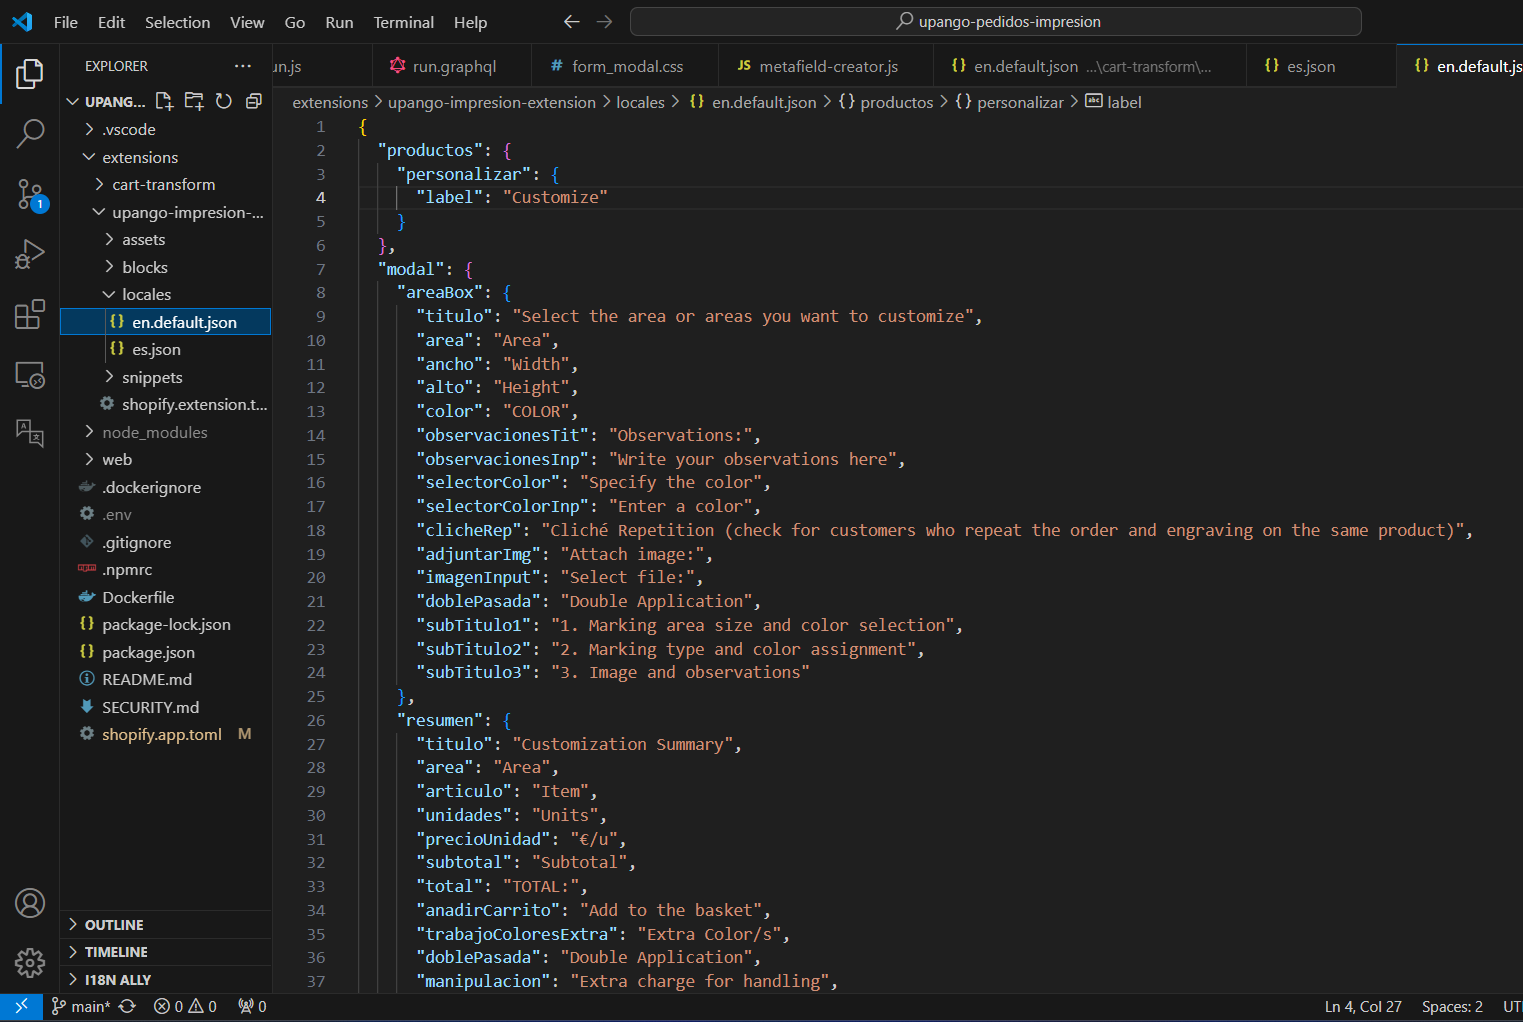
\includegraphics[width=0.8\textwidth]{imagenesUS1/locales.png}
    \caption{\label{fig:locales}Ficheros locales}
    \vspace{\fill}
\end{figure}

Por lo que respecta a la creación y apertura del modal, se ha tomado la decisión de generar dinámicamente el contenido del mismo y su funcionalidad
asociada mediante JavaScript. El uso de JavaScript permite una interacción más fluida y una mejor experiencia de usuario. Además, al tener acceso directo 
a los valores y elementos necesarios, se pueden realizar los cálculos y validaciones de manera directa y eficiente, porporcionando una personalización
más precisa y completa. El hecho de que el modal tenga tanta funcionalidad, datos y elementos cambiantes según la interacción del usuario, hace que 
el empleo de JavaScript para implementarlo sea una buena opción para facilitar ese acceso a datos y cambios dinámicos del contenido del modal.
Esta estrategia también simplifica el mantenimiento del código, al centralizar todas las funciones relacionadas con el modal en un solo lugar, lo que facilita
futuras actualizaciones y mejoras. Debido a esta decisión tanto el contenido como la funcionalidad de este modal se han desarrollado en un mismo fichero javaScript.

Antes de proceder con la creación e implementación de funcionalidad del modal, se han implementado unas funciones en la sección \textit{botonPersonalizar.liquid} que emplean liquid para crear e inicializar unas estructuras JavaScript que 
contendrán todos los datos relevantes del producto de impresión, así como todos los textos traducidos necesarios para crear el modal y sus elementos. El acceso a datos que proporciona liquid permite poder crear 
esta estructura para tener los datos disponibles en el modal sin necesidad de realizar llamadas adicionales al Admin API. Estas funciones serán llamadas desde el fichero 
javaScript que maneje la funcionalidad y creación del modal para inicializar y tener acceso a todos los datos en caso de que lo necesite.

En la Figura~\ref{fig:cargarlocales} se puede observar la función \textit{cargarLocales()} al ejecutar esta función, la estructura \textit{localesModal} se carga con 
todas las traducciones de textos que deben aparecer en el modal, pues desde javascript no tenemos acceso directo a esta funcionalidad de archivos locales para la implementación 
de la experiencia multilingüe.

\begin{figure}[ht]
    \floatplacement{figure}{!t}
    \centering
    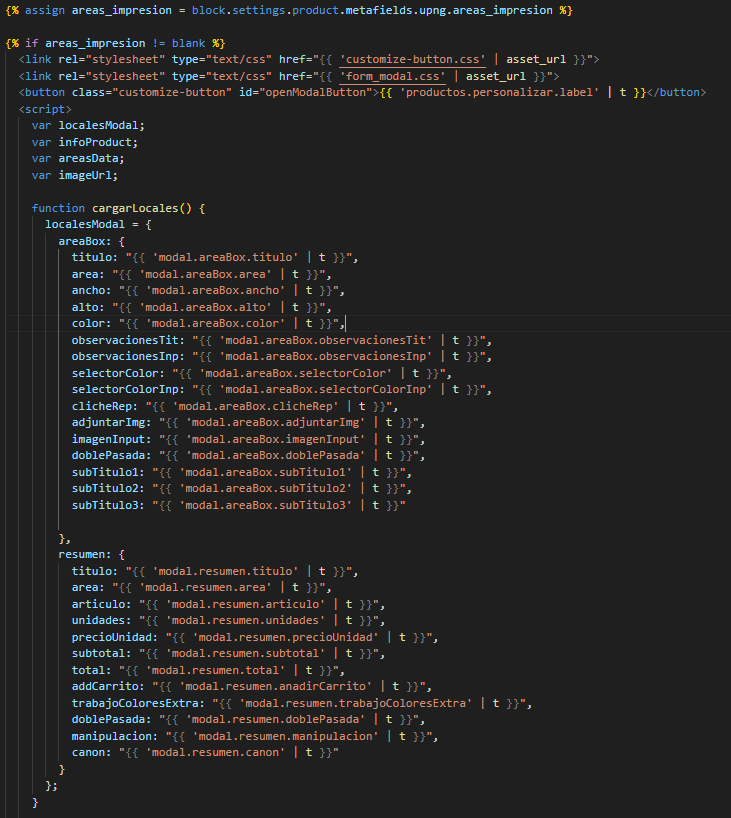
\includegraphics[width=0.8\textwidth]{imagenesUS3-section/funcioncargarLocales.png}
    \caption{\label{fig:cargarlocales} Función para almacenar locales en estructura javaScript}
    \vspace{\fill}
\end{figure}

En la Figura~\ref{fig:cargardatos} se puede ver la implementación de la función \textit{almacenarDatosProductos()}. Esta desempeña un papel crucial en 
la recopilación y estructuración de la información sobre el producto actual de la tienda. En esta se recopilan y almacenan en la estructura \textit{infoProduct} los datos generales del producto, como su nombre, precio, identificador y cantidad de
unidades seleccionada. Después itera sobre las áreas de impresión del producto, obteniendo detalles como el nombre, dimensiones, imágenes, trabajos asociados con todos sus elementos, cliches asociados a los trabajos y toda la información necesaria. Esta función
almacena todos los datos de las áreas del producto en la estructura \textit{areasData}.


\begin{figure}[ht]
    \floatplacement{figure}{!t}
    \centering
    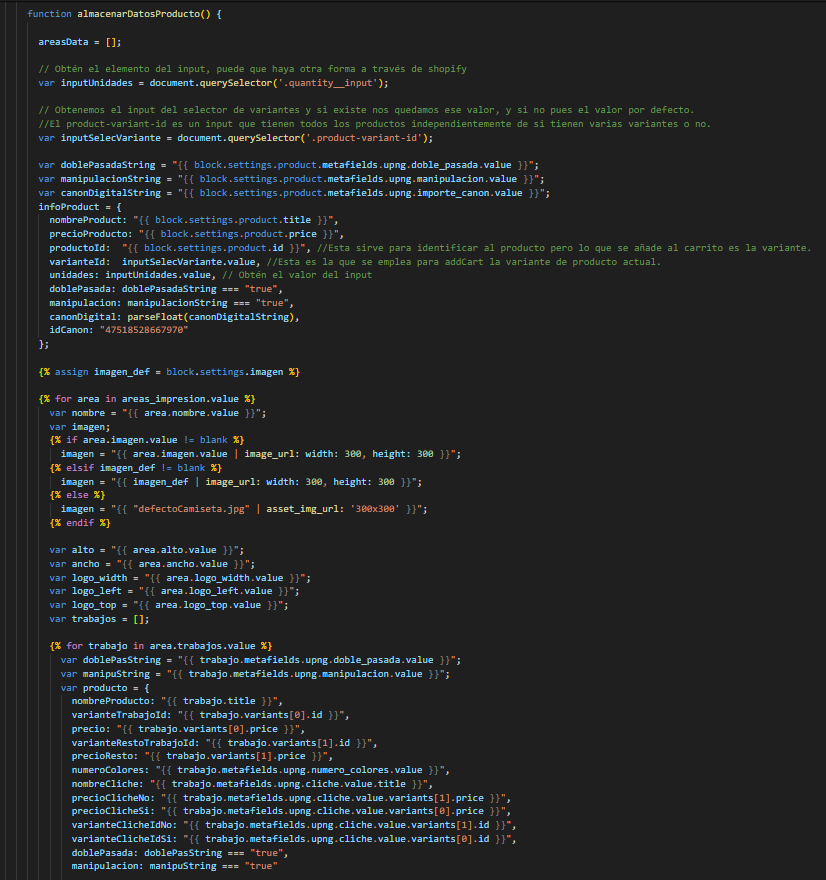
\includegraphics[width=0.8\textwidth]{imagenesUS3-section/funcionAlmacenarDatosProductos.png}
    \caption{\label{fig:cargardatos} Función para almacenar datos en estructura javaScript}
    \vspace{\fill}
\end{figure}

En esta sección también se pueden destacar las líneas que importan los archivos JavaScript necesarios, entre los que se debe destacar
el fichero \textit{ventanta-modal.js}, este se carga de manera diferida para optimizar el rendimiento, y es el script en el que se ha desarrollado toda la funcionalidad y creación del
personalizador (modal) (Figura~\ref{fig:finalSeccion}). También destacar que en esta sección se encuentran otras líneas que importan archivos CSS que se emplean en la aplicación para aplicar estilos 
a los elementos de la página como los botones o los elementos del modal (Figura~\ref{fig:creacionSeccion}).

\begin{figure}[ht]
    \floatplacement{figure}{!t}
    \centering
    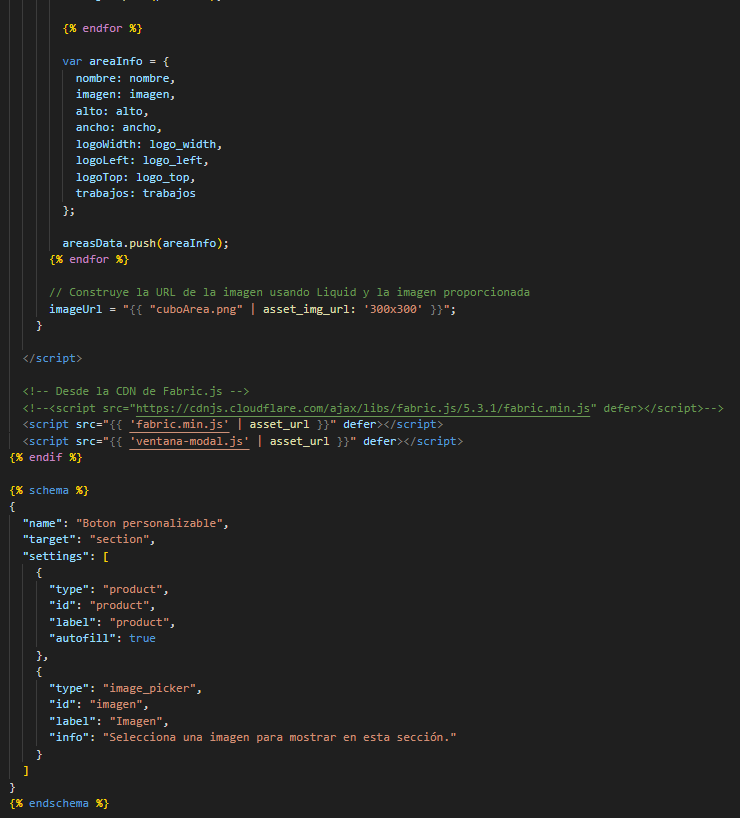
\includegraphics[width=0.8\textwidth]{imagenesUS3-section/finalSeccion.png}
    \caption{\label{fig:finalSeccion} Final de sección \textit{botonPersonalizar.liquid}}
    \vspace{\fill}
\end{figure}

Una vez implementada toda la funcionalidad en la sección \textit{botonPersonalizar.liquid} ya se puede proceder con la implementación de la ventana
modal y toda su funcionalidad asociada.

En primer lugar, en la Figura~\ref{fig:iniciojs} se puede observar un evento que engloba a todo el contenido del fichero. Este evento se dispara cuando el DOM (Modelo de Objetos del Documento) ha 
sido completamente cargado y analizado, lo que garantiza que el código dentro de la función se ejecute una vez que la página esté lista. Esto se emplea para evitar errores.
A continuación se obtiene mediante su identificador, el botón ``Personalizar'' encargado de abrir el modal. Y posteriormente se crea el contenedor ``div'' que albergará 
todo el contenido y funcionalidad. Este contarará con todos los estilos CSS que se han creado e importado para darle un aspecto de ventana modal. Del mismo modo, todos los elementos
creados, cuentan con clases de estilos implementadas en los dos ficheros CSS que se han creado para este proyecto \textit{form-modal.css} y \textit{customize-button.css}.

Después en la Imagen~\ref{fig:finaljs} se puede ver como se ha creado la función \textit{openModal()}. Esta es la función principal que se encarga
de generar y mostrar el modal. En primer lugar se establece el estilo CSS del elemento ``customModal'' (contenedor del modal) para que sea visible (``display:block'').
Luego, se vacía el contenido HTML dentro de este modal para asegurarse de que esté limpio y listo para generar dinámicamente y mostrar todo el contenido de este modal.
A continuación, se realizan varias llamadas a funciones: Se llama a ``cargarLocales()'' para cargar las traducciones locales necesarias, ``almacenarDatosProductos()'' para que se generen
y se almacenen las estructuras de datos necesarios para la generación de este modal, y por último se llama a ``generateAreaTable()'' para generar todo el contenido y funcionalidades
del modal. 

Al final del documento se agrega un event listener al botón ``Personalizar'' que activa la apertura del modal. De forma que cuando se haga clic en este botón, se 
ejecute la función ``openModal()'', mostrando el modal con todos sus elementos y funcionalidad asociada.

En la función \textit{generateAreaTable()} se ha realizado toda la implementación de elementos y funcionalidad. En el comienzo de esta función (Figura~\ref{fig:iniciojs}) se puede destacar la creación del botón
``closeModalButton'' que se empleará para cerrar la ventana modal. En la Figura~\ref{fig:finaljs} se observa como al final de la función se ha creado un eventListener para este botón, que se mantiene en espera de un evento
click para realizar una llamada a la función \textit{closeModal()} que es la encargada de ocultar el modal mediante la modificación de su visibilidad.

\begin{figure}[ht]
    \floatplacement{figure}{!t}
    \centering
    \includegraphics[width=0.8\textwidth]{imagenesUS3-modal/AbrirModalPrimeraParte y función generateAreaTable.png}
    \caption{\label{fig:iniciojs} Creación de la ventana modal en \textit{ventana-modal.js}}
    \vspace{\fill}
\end{figure}



\begin{figure}[ht]
    \floatplacement{figure}{!t}
    \centering
    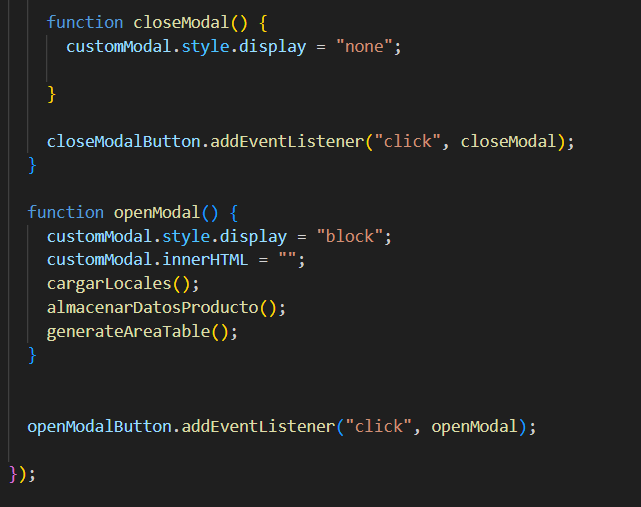
\includegraphics[width=0.8\textwidth]{imagenesUS3-modal/FinalDeOpenModal.png}
    \caption{\label{fig:finaljs} Apertura y generación del modal en \textit{ventana-modal.js}}
    \vspace{\fill}
\end{figure}




\clearpage
\subsubsection{Implementación del frontend de la parte de administración}

\clearpage
\subsubsection{Implementación del backend}

\clearpage
\subsubsection{Implementación de customize bundles y modificación de tema}
En esta sección se mostrará la investigación e implementación de los ``customize bundles'' para agrupar y vincular los
productos de los paquetes de impresión. Una vez añadidos los productos al carrito, esta funcionalidad permitirá relacionar en paquetes, los productos de los pedidos personalizados, de forma que no se puedan borrar
o editar por separado. Además, se realizará una nueva versión de la sección de desglose de artículos del carrito. Esto se debe a que en el tema estandar no se muestran los artículos de un paquete 
de impresión. En esta, se pinta un solo elemento con el precio total del conjunto. El usuario final debe poder visualizar en el carrito un desglose de los paquetes con todos los artículos que incluye y su precio 
total para obtener una buena experiencia de compra.

Las \textbf{funciones de Shopify} \cite{shopify-functions} permiten a los desarrolladores personalizar la lógica del backend de Shopify, incluyendo casos de uso como la implementación de los
``customize bundles''. Estas funciones se basan en destinos de extensión que inyectan código en la lógica de backend de Shopify. La entrada de estas funciónes es un objecto JSON resultado de una
consulta de GraphQL, permitiendo seleccionar datos específicos como los de la línea de carrito en este caso. La lógica de la funcion se realizará en JavaScript, y se compila en módulos de WebAssembly.
La salida de esta función es un documento JSON que describe las operaciones deseadas y que Shopify se encargará de interpretar. Además Shopify proporciona esquemas que especifican los 
destinos, entradas y salidas esperadas para la API de Functions.

En este caso se usarán estas funciones para realizar una modificación del carrito. Para ello, mediante la Shopify CLI se debe crear en la aplicación una extensión de transformación de carrito. Esta proporciona 
la estructura básica para poder definir la query y la función que ejecutará y devolverá el resultado JSON con las operaciones de modificación a Shopify (Figura~\ref{fig:estructuracarttrans}). 

\begin{figure}[ht]
    \floatplacement{figure}{!t}
    \centering
    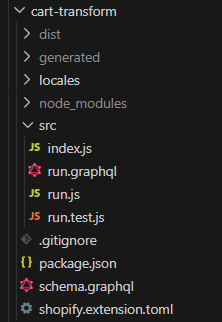
\includegraphics[width=0.3\textwidth]{imagenes-tema/estructuraCartTransform.png}
    \caption{\label{fig:estructuracarttrans} Estructura de la extensión \textit{cart-transform}}
    \vspace{\fill}
\end{figure}

Una vez creada la extensión \textit{cart-transform}, se debe configurar la query de la consulta GraphQL cuyo resultado será la entrada de la función. Esta consulta (Figura~\ref{fig:queryCart}) está diseñada para obtener
información detallada sobre los elementos del carrito de la tienda. En este caso, se solicitan datos como el identificador de la línea de carrito, la cantidad, una serie de propiedades que se han introducido al añadir los productos personalizados 
y que servirán para localizar los elementos que deben pertenecer a un mismo paquete y poder asociarlos, y también se recupera el 
metafield \textit{importe-canon} con el que pueden contar algunos productos y que servirá para aplicar el impuesto canon digital.


\begin{figure}[ht]
    \floatplacement{figure}{!t}
    \centering
    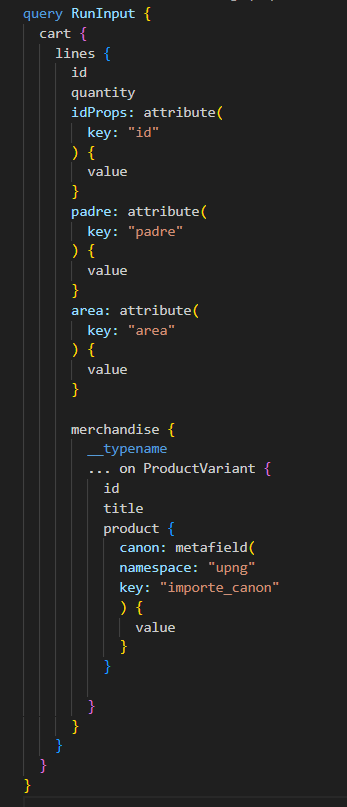
\includegraphics[width=0.2\textwidth]{imagenes-tema/queryCartTransform.png}
    \caption{\label{fig:queryCart} Fichero \textit{run.graphql}}
    \vspace{\fill}
\end{figure}

Por lo que respecta a la implementación de la función, esta se divide en dos partes principales: la primera parte (Figura~\ref{fig:runpart1})  se encarga de procesar las las líneas de carrito que contienen
propiedades definidas (artículos de personalización), mientras que la segunda parte se encarga de las líneas del carrito que no tienen propiedades definidas (artículos normales sin personalización).

En la primera parte, se filtran las líneas del carrito que tienen la propiedad 'idProps' y 'value' definidas, y se agrupan según su identificador. Si una línea comparte el mismo identificador que la anterior
o es la primera línea del carrito, se agregan a una estructura de datos que representa un grupo de líneas. Cuando se encuentra una línea con un identificador diferente, se crea una nueva operación 
que combina las líneas del grupo anterior y se reinicia el proceso para el nuevo grupo. Con este procedimento se generan una serie de operaciones de tipo ``merge'' que se van añadiendo al array de operaciones que retorna 
la función. Estas operaciones serán interpretadas por el backend de Shopify y resultarán en una transformación del carrito que mostrará los items de un mismo producto de personalización asociados.

En la segunda parte (Figura~\ref{fig:runpart2}), se procesan las líneas del carrito que no tienen propiedades definidas, que corresponden a productos que no son personalizados. Estos productos se recorren y en función de si cuentan con canon digital o no, se expanden agregando 
el producto especial canon con su cantidad correspondiente. Con este procedimiento se generan una serie de operaciones de tipo ``expand'' que se van añadiendo al array de operaciones. Este tipo de operaciones
serán interpretadas por el backend de Shopify y resultarán en una transformación del carrito que añadirá el canon digital a los productos normales que deban contar con él, asociados en un mismo paquete. Es decir, esta operación añade los productos canon al carrito
y los asocia con los productos no personalizados correspondientes.

Como último paso para activar esta funcionalidad en la tienda en la que se instale la aplicación, habría que ejecutar una mutación GraphQL para crear un objeto de tipo \textit{cart-transform}, que cuente con el identificador de la función que se ha implementado
y que se debe aplicar. Este objeto es el encargado de llamar a la función de transformación correspondiente cuando el usuario entra al carrito de la tienda.

\begin{figure}[ht]
    \floatplacement{figure}{!t}
    \centering
    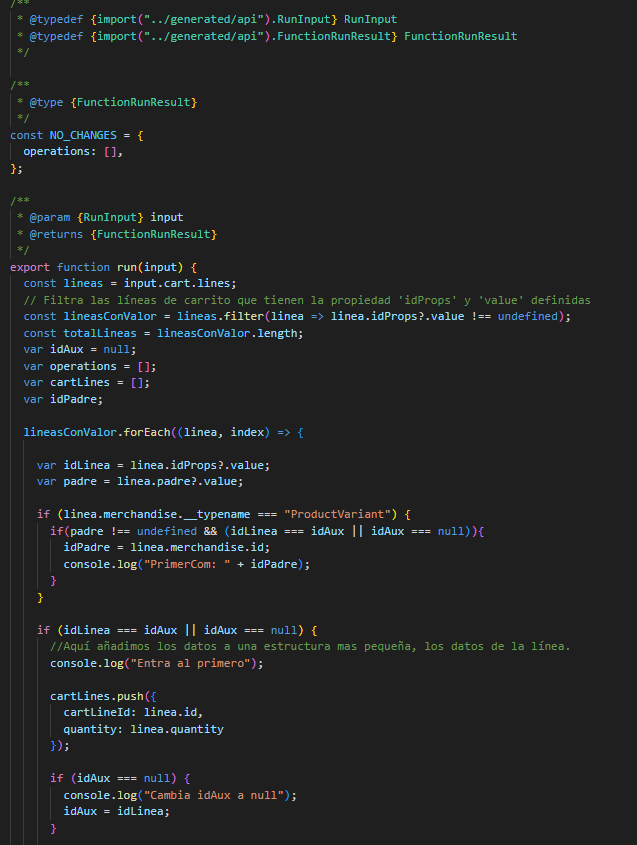
\includegraphics[width=0.4\textwidth]{imagenes-tema/primeraParteFunction.png}
    \caption{\label{fig:runpart1} Funcionalidad para crear paquetes de impresión} 
    \vspace{\fill}
\end{figure}

\begin{figure}[ht]
    \floatplacement{figure}{!t}
    \centering
    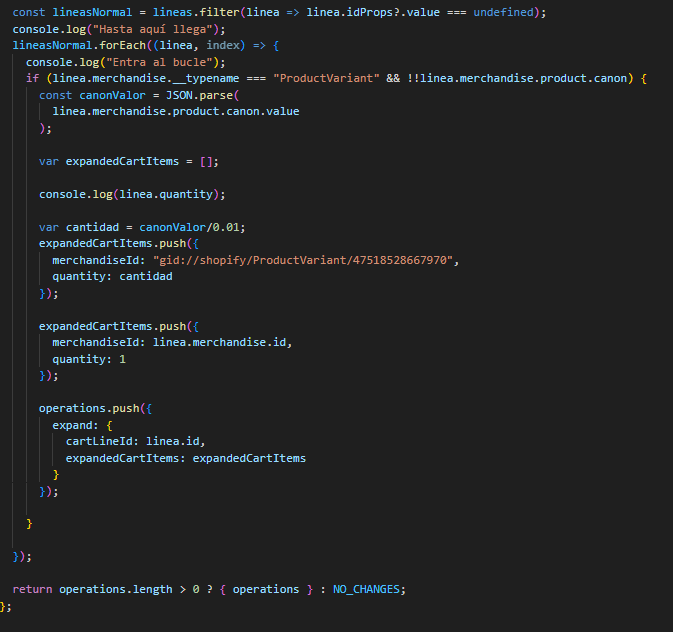
\includegraphics[width=0.5\textwidth]{imagenes-tema/segundaParteFunction.png}
    \caption{\label{fig:runpart2} Funcionalidad para añadir canon digital} 
    \vspace{\fill}
\end{figure}

Al aplicar los customize bundles, se observa que los paquetes de productos de personalización, no muestran los detalles de los artículos que contienen. Estos 
paquetes se muestran como un solo artículo de tipo paquete cuyo contenido no está visible. Por ello se ha implementado una nueva sección en un tema estandar en el que 
se desglose el contenido de este paquete (Figura~\ref{fig:seccionTema}).

Esta es una versión actualizada de la sección \textit{main-cart-items.liquid}. En ella (Figura~\ref{fig:modificacionTema}) se recorren los 
elementos de los item que contienen otros artículos (paquetes) y se van imprimiendo todos estos productos que contiene. Se emplea liquid para mostrar sus precios, imágenes y toda la información pertinente,
con el objetivo de mejorar la experiencia del usuario.

\begin{figure}[ht]
    \floatplacement{figure}{!t}
    \centering
    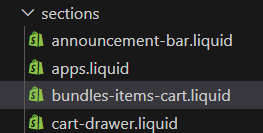
\includegraphics[width=0.5\textwidth]{imagenes-tema/creacionSeccionTema.png}
    \caption{\label{fig:seccionTema} Nueva versión de la sección \textit{main-cart-items.liquid}} 
    \vspace{\fill}
\end{figure}

\begin{figure}[ht]
    \floatplacement{figure}{!t}
    \centering
    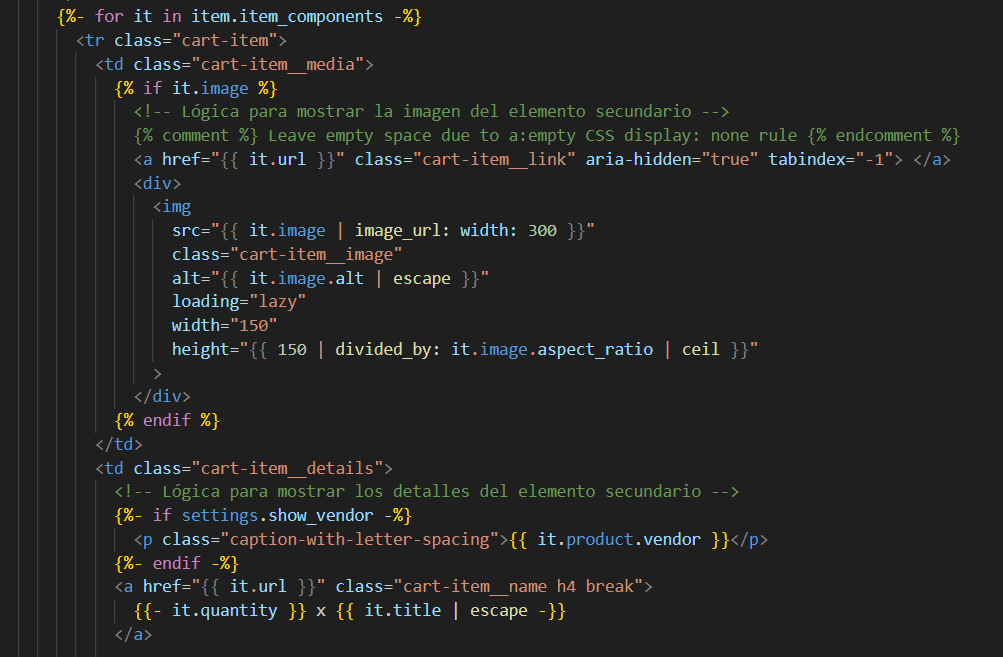
\includegraphics[width=0.8\textwidth]{imagenes-tema/modificaciondetema.png}
    \caption{\label{fig:modificacionTema} Modificación de la sección \textit{main-cart-items.liquid}} 
    \vspace{\fill}
\end{figure}


\clearpage
\subsection{Pruebas}
En cuanto a las pruebas realizadas, a lo largo de todo el proceso de desarrollo de la aplicación, se han ido llevando a cabo pruebas continuas
con el objetivo de verificar el correcto funcionamiento de las funcionalidades implementadas. Estas pruebas se han ido realizando de manera manual 
a medida que se iban complentando las diferentes tareas definidas para cada historia de usuario, de modo que la aplicación iba creciendo en funcionalidades 
a la par que se comprobaba su correcto funcionamiento.

Cada vez que se implementaba una nueva funcionalidad, se realizaban pruebas exhaustivas para asegurar su correcto funcionamiento antes de proceder con la 
siguiente tarea. Estas pruebas se han enfocado en verificar el correcto funcionamiento tanto del frontend como del backend, pues como se ha comentado anteriormente, 
el desarrollo de ambas partes se ha ido realizando de forma conjunta.

Es importante destacar que se optó por la realización de pruebas manuales en lugar de la implementación de pruebas automatizadas debido a que se 
trata de una aplicación relativamente pequeña y con una funcionalidad en la parte de backend bastante limitada. Se consideró que el esfuerzo necesario y la inversión
en tiempo y recursos para establecer pruebas automatizadas no justificaba su implementación. Esta decisión permitio una mayor flexibilidad y agilidad durante
el proceso de desarrollo de la aplicación.

Para realizar las pruebas manuales a la par que se iban desarrollando las funcionalidades de la aplicación, se ha hecho uso de \textbf{Nodemon}. 
Esta es una herramienta de línea de comandos para Node.js, cuya función principal es monitorizar los archivos del proyecto y reiniciar autómaticamente
la aplicación cuando se detectan cambios en el código fuente \cite{nodemon}. 
Esta herramienta ha eliminado la necesidad de detener y reiniciar manualmente el servidor cada vez que se han realizado modificaciones en el código, 
lo que ha agilizado el proceso de desarrollo y ha permitido comprobar el funcionamiento de cada tarea a la par que se implementaba, pues permitía observar como
cada cambio reciente se reflejaba automáticamente.

El uso de nodemon, ha facilitado tanto la implementación y pruebas de la parte de frontend como la de backend. En cuanto a la parte del frontend
ha permitido ir creando funcionalidades y dando diseño a esta parte, puediendo observar los resultados de cada cambio en el código en tiempo real,
lo que ha agilizado muchisimo el desarrollo. Por lo que respecta al backend mas de lo mismo, se han podido ir realizando modificaciones y pruebas de las funcionalidades
hasta conseguir el resultado esperado, permitiendo solucionar los errores, mejorar el código y probarlo de forma muy ágil y rápida. 

Se ha hecho uso de \textbf{Postman} para llevar a cabo las pruebas de los EndPoints de la parte del backend, esta plataforma ha permitido enviar 
solicitudes HTTP a los EndPoints de la aplicación, permitiendo así verificar la correcta funcionalidad de los servicios web. Asimismo, una vez implementadas
las llamadas desde la parte del frontend, se realizaron pruebas adicionales para garantizar la correcta comunicación entre backend y frontend y asegurando una
experiencia del usuario fluida y sin errores.

Por último añadir que durante todo el proceso de desarrollo, se han ido realizando pruebas de la parte del frontend del tema (theme app extensión) en diversos
navegadores para probar la aplicación desde diferentes entornos y permitir identificar problemas de compatibilidad y rendimiento.
Además se ha hecho uso de una herramienta clave con la que cuentan la mayoría de navegadores, que proporciona la capacidad de simular diferentes 
tamaños de pantalla y dispositivos actuales, lo que ha facilitado el poder probar el diseño responsive de esta aplicación a lo largo del desarrollo.

\subsection{Despliegue}
Hasta la fecha, en Upango no se ha recibido ninguna solicitud por parte de los clientes que requiera hacer uso de las funciones de personalización de productos
que ofrece esta aplicación. Dado que no se ha tenido la necesidad de implementar esta aplicación en las tiendas en desarrollo para los clientes hasta el momento, tampoco ha sido 
necesario contratar los servicios de una empresa de hosting y desplegarla en un servidor privado. Del mismo modo, tampoco se ha adquirido un dominio web público 
específico para esta aplicación.

Por esta razón, se ha desplegado esta aplicación de manera local y haciendo uso de las herramientas que proporciona Shopify. Para desplegar la aplicación,
se han aprovechado las funcionalidades de la Shopify CLI. Esta herramienta cuenta con una interfaz de línea de comandos que proporciona diversas funcionalidades para desplegar la aplicación.
Empleando la Shopify CLI, se ha ejecutado el comando \textit{npm run dev} que ejecuta el script definido en el archivo package.json bajo la clave dev. En este caso como se muestra en la Figura~\ref{fig:scriptsPackageJson} se estaría ejecutando \textit{shopify app dev} el cual es el comando específico para lanzar la aplicación.
Este al ejecutarse inicia un servidor local tanto para el backend como para el frontend, proporcionando
una dirección URL pública temporal la cual Shopify se encarga de gestionar automáticamente actualizándola según sea necesario. Esta URL permite lanzar y compartir esta aplicación para probarla durante el desarrollo, con la ventaja de que 
Shopify se encarga de gestionar su seguridad y privacidad.

\begin{figure}[ht]
    \floatplacement{figure}{!t}
    \centering
    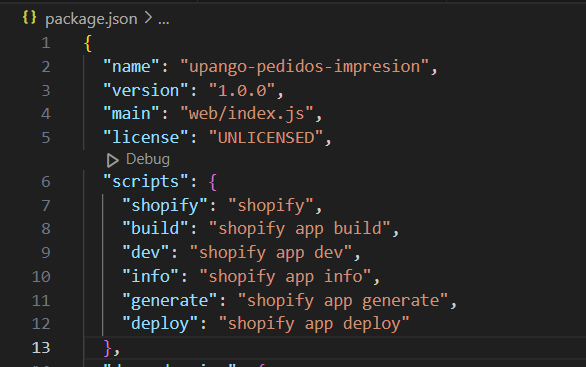
\includegraphics[width=0.8\textwidth]{imagenes/package.json.scripts.png}
    \caption{\label{fig:scriptsPackageJson}package.json}
    \vspace{\fill}
\end{figure}

En este proceso de despliegue, se hace uso de Cloudflare, concretamente de la funcionalidad Cloudflare Tunnel. Esta funcionalidad permite exponer servicios que se ejecutan
en una infraestructura local a través de la red de Cloudflare, lo que proporciona una capa adicional de seguridad y rendimiento, pues en lugar de 
exponer directamente los servidores locales a internet, los túneles de Cloudflare establecen una conexión segura a través de la red de Cloudflare y protege los
servidores de posibles ataques maliciosos, proporcionando una mayor confiabilidad en la entrega de contenido \cite{cloudflare}. 

Al crear un túnel entre el entorno local y la tienda de desarrollo y pruebas empleando Cloudflare, se puede permitir que los servicios que se ejecutan en la infraestructura local
sean accesibles a través de internet de una manera segura y aprovechándo la gran infraestructura de red global con la que cuenta Coudflare para enrrutar el tráfico.

En el caso de que los clientes de Upango solicitasen los servicios de esta aplicación y se necesitase hacer un despliegue real, se seguiría el siguiente procendimiento que ya se ha utilizado para
desplegar otro tipo de aplicaciones.
En primer lugar se contratarían los servicios de hosting para alojar la aplicación en un servidor y habría que hacerse con un dominio o subdominio
que esté apuntando a ese servidor. Una vez obtenido el servidor, habría que conectarse a el mediante SSH para proceder a configurarlo. En este caso para trabajar cómodamente en este servidor remoto,
se haría uso de herramientas como \textbf{Remote Explorer} y \textbf{Remote SSH}, estas son extensiones de Visual Studio Code que permiten trabajar de una manera mas eficiente y comoda con los archivos del
servidor empleando el editor de código. Estas herramientas facilitan la conexión al servidor, las configuraciones y despliegue de aplicaciones que se realizan en él, y a la hora 
de tener que analizar errores y solucionarlos una vez la aplicación está en producción, amenizan estas tareas de manipular el código.

Estando ya dentro del servidor, es necesario instalar varias herramientas esenciales, si no están presentes en este. Entre ellas se pueden destacar un servidor web como \textbf{Apache}, que es fundamental para servir la aplicación
al público; \textbf{npm} y \textbf{Node.js} que permitirán ejecutar el código JavaScript en el servidor y administrar las dependencias del proyecto a través de npm; \textbf{Git}, para poder descargar el código fuente de la aplicación desde 
el repositorio remoto y en caso realizar modificaciones en el código del servidor poder actualizarlo en el repositorio; y \textbf{pm2}, un administrador de 
procesos para aplicaciones Node.js que garantiza que las aplicaciones se ejecuten de manera continua gestionando múltiples instancias y permitiendo su reinicio en caso de fallos.
Una vez vez preparado el entorno, se descarga la aplicación desde el repositorio remoto y se instalan las dependencias necesarias ejecutando \textit{npm install}. Despues se deben buscar las variables de entorno que genera y configura Shopify al crear una aplicación,
estas se pueden obtener de varias maneras, o bien a través del panel de partners de Shopify o introduciendo el comando \textbf{npm run shopify app env show}. En la Figura~\ref{fig:VariablesEntorno} se pueden observar dichos tokens. Para poder 
tener diferentes aplicaciones en el servidor con distintas variables, en lugar de crear variables de entorno como tal, se deben pasar como parámetros al proceso de node.

\begin{figure}[ht]
    \floatplacement{figure}{!t}
    \centering
    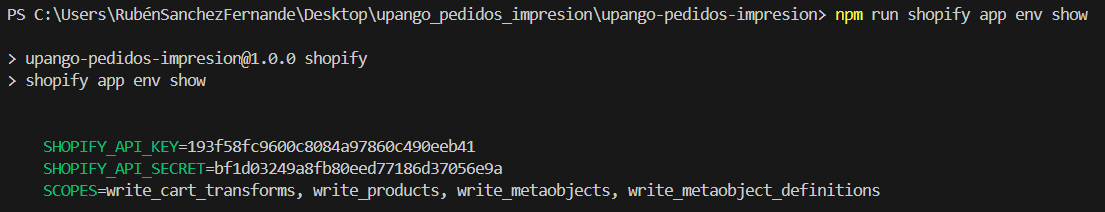
\includegraphics[width=0.8\textwidth]{imagenes/variablesEntornoDespliegue.png}
    \caption{\label{fig:VariablesEntorno}Variables de entorno de la aplicación}
    \vspace{\fill}
\end{figure}

A continuación se procede a compilar los archivos del frontend, pues en producción es necesario compilar los ficheros de react que hay en el directorio \textit{web/frontend} 
para generar la carpeta \textit{web/frontend/dist} que contiene los compilados. Al hacer esto, hay que ejecutar \textit{npm install} para instalar las dependencias del frontend como vite,
se indica el valor de la siguiente variable de entorno que necesita para compilar \textit{export SHOPIFY\_API\_KEY=193f58fc9600c8084a97860c490eeb41} y por último hay que ejecutar \textit{npm run build} para realizar
la compilación.

Una vez hecho esto ya se puede ejecutar la aplicación en modo producción, para ello se debe ejecutar el comando \textit{npm run serve} desde el directorio \textit{web}. Se debe acompañar
a este comando de unos parámetros para que cuente con sus variables de entorno, estas variables son la SHOPIFY\_API\_KEY, el SHOPIFY\_API\_SECRET, los SCOPES,  el host, es decir la url de la app y el puerto.

Además para que la app esté siempre en ejecución, es necesario lanzar el comando npm run serve con sus variables a través de un pm2 start y añadiendo un parámetro name al final para
darle un nombre al proceso y poder identificarlo y gestionarlo. 

Llegados a este punto quedaría configurar el dominio de la aplicación en el servidor, para ello primero es necesario modificar la configuración del servidor web Apache en este caso, para que 
el dominio apunte al servidor y se haga un mapeo al puerto correspondiente de la aplicación. Esto implica editar archivos de configuración del servidor como el archivo \textit{http\_node.conf}. 
A continuación se deben crear y configurar los certificados SSL para admitir HTTPS, empleando herramientas como Let's Encrypt para generar certificados gratuitos. Una vez configurados los
certificados, se actualiza la configuración del servidor para que acepte conexiones HTTPS en el puerto 443. Una vez hecho esto hay que reiniciar Apache para que los cambios surtan
efecto y la aplicación pueda ser accedida correctamente a través del dominio configurado.

Por último, se debe ajustar la configuración de la aplicación desde el panel de administración de partners para que la aplicación reconozca el nuevo dominio (Figura~\ref{fig:ConfiguracionAppPartner}) y generar un enlace de instalación de esta aplicación
para instalarla en la tienda que lo solicite (Figura~\ref{fig:DistributionAppPartners}, Figura~\ref{fig:generarLinkDistribution}).

\begin{figure}[ht]
    \floatplacement{figure}{!t}
    \centering
    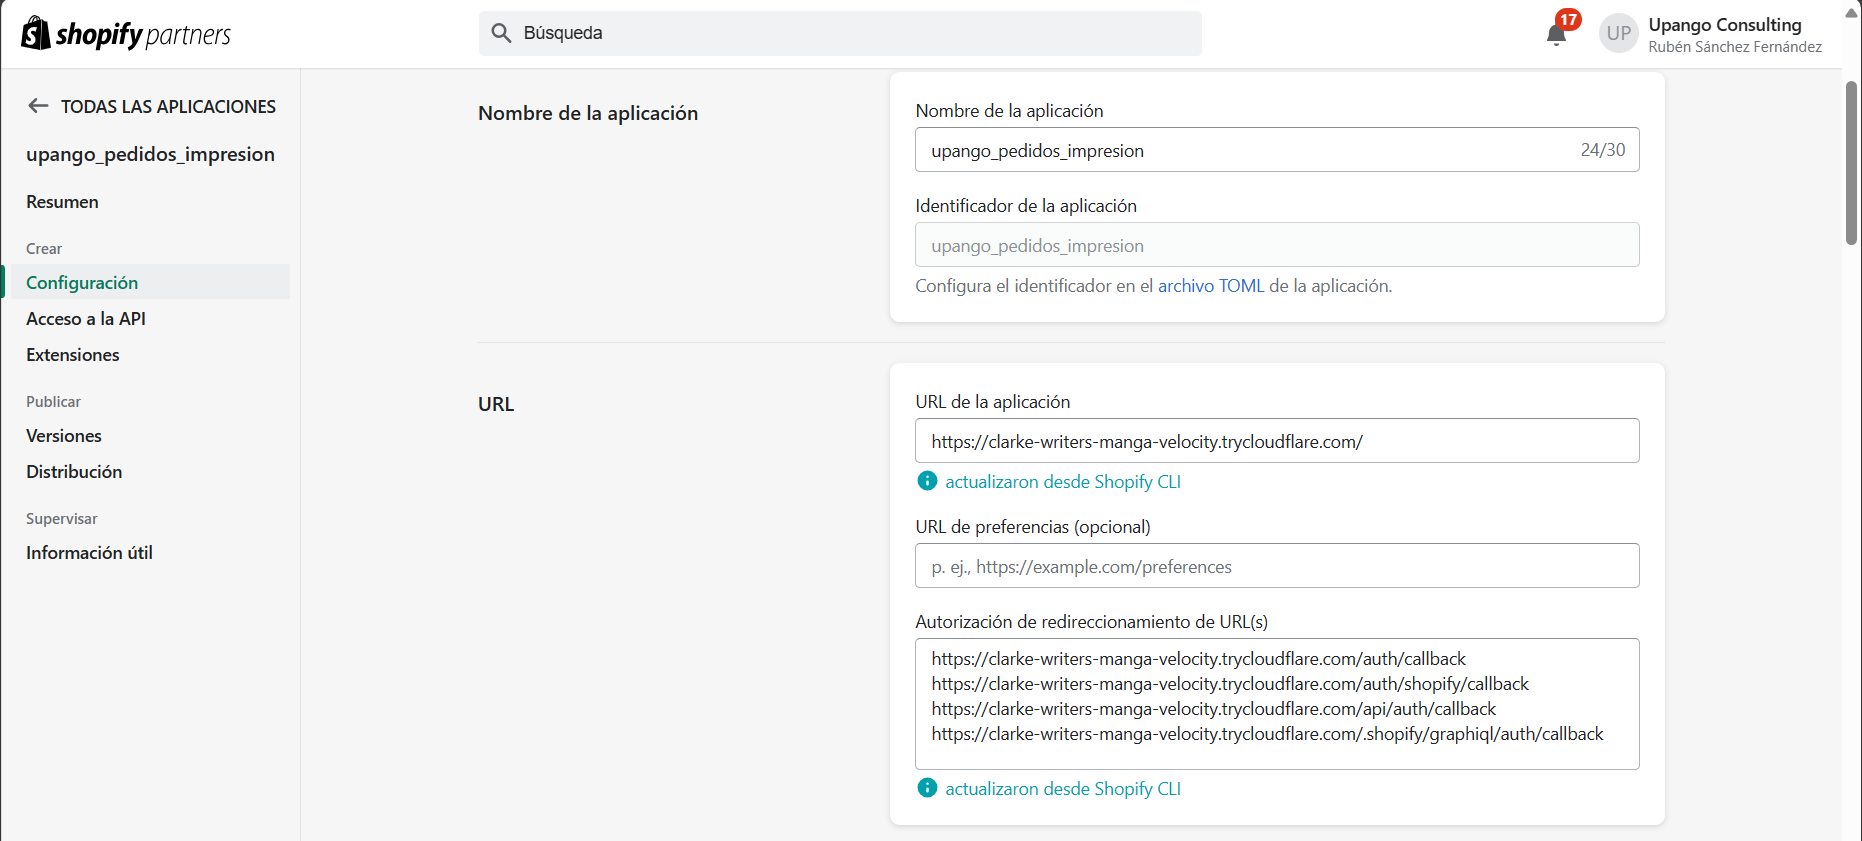
\includegraphics[width=0.8\textwidth]{imagenes/panelPartnersDistribution.png}
    \caption{\label{fig:ConfiguracionAppPartners}Configuración de la aplicación}
    \vspace{\fill}
\end{figure}

\begin{figure}[ht]
    \floatplacement{figure}{!t}
    \centering
    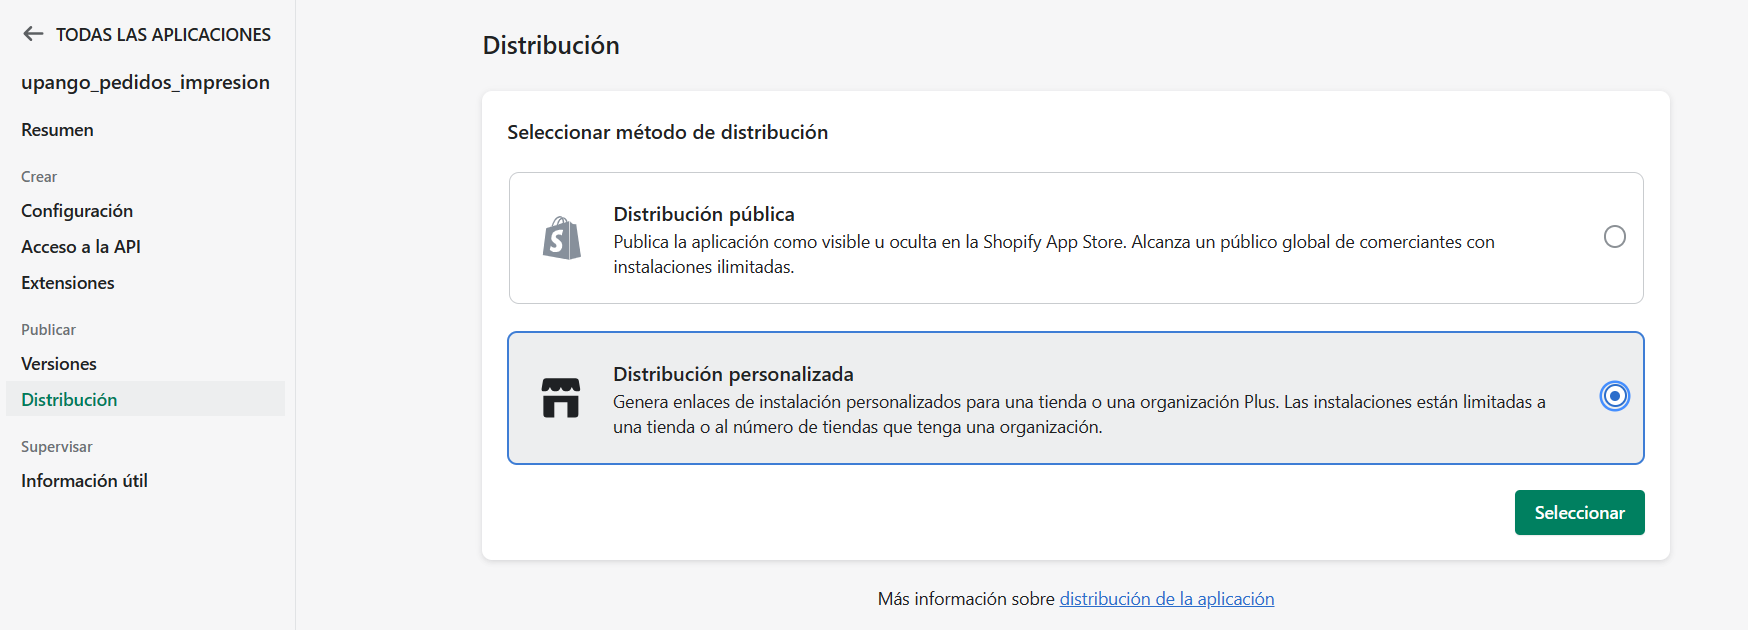
\includegraphics[width=0.8\textwidth]{imagenes/distribucionAppEnlace.png}
    \caption{\label{fig:DistributionAppPartners}Distribución de la aplicación}
    \vspace{\fill}
\end{figure}

\begin{figure}[ht]
    \floatplacement{figure}{!t}
    \centering
    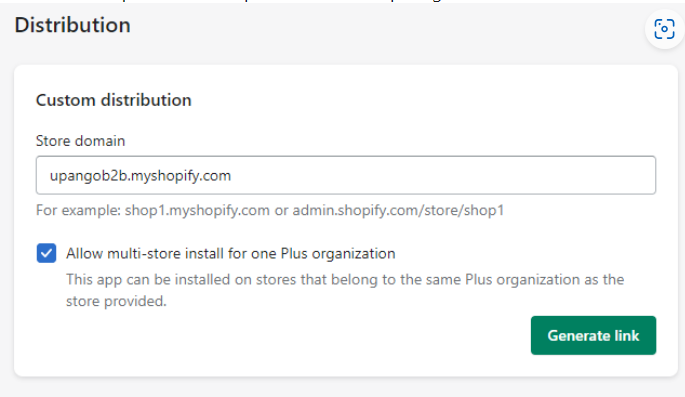
\includegraphics[width=0.8\textwidth]{imagenes/generarLinkDistribution.png}
    \caption{\label{fig:generarLinkDistribution}Generar link de distribución}
    \vspace{\fill}
\end{figure}


\clearpage
\section{Conclusiones y vías futuras}

\subsection{Conclusiones}
A modo de conclusión se puede decir que en este Trabajo de Fin de Grado (TFG) se han logrado cumplir todos
los objetivos propuestos inicialmente. Se ha diseñado y desarrollado una aplicación para la plataforma Shopify que 
permite la personalización de productos para su posterior compra en las tiendas de los clientes que la empleen.
Desde el análisis inicial hasta la implementación y despliegue, se ha seguido una metodología estructurada que ha permitido
alcanzarar cada hito de manera efectiva y eficiente.

Además se ha desarrollado una aplicación con unas funcionalidades estandar al mercado y a los posibles requisitos que podrían solicitar en un futuro
los clientes. Se ha implementado de forma estandarizada, de tal manera que este preparada para añadir y modificar las funcionalidades facilmente, lo que la hace
adaptable a los requisitos de futuros clientes que pueden necesitar características especificas de esta herramienta.
Se ha creado una base sólida sobre la cual poder construir y expandir la aplicación según las necesidades del mercado y los clientes.

El análisis detallado de los objetivos, la metodología ágil implementada y el enfoque iterativo e incremental que se ha aplicado,
ha sido fundamental no solo para cumplir con los requisitos establecidos, sino también para anticiparse a las posibles necesidades futuras y
preparar la aplicación para seguir creciendo de manera continua, aplicando mas iteraciones.

\subsection{Trabajo futuro}
En el ámbito del desarrollo futuro, la aplicación se vislumbra como un proyecto en constatne evolución y mejora. Actualmente, su estructura básica se ha 
establecido en función de los requisitos de proyectos previos de la empresa y las necesidades específicas de los clientes en ese momento. Sin embargo, su 
verdadero potencial radica en su capacidad de adaptación y expansión para satisfacer las demandas cambiantes del mercado y las preferencias individuales de los 
clientes venideros.

Es importante resaltar que la aplicación, en su forma actual, no representa el producto final, sino más bien una versión estándar adaptable que servirá como punto
de partida para futuros desarrollos. Se concibe como una base sólida sobre la cual se construirán soluciones personalizadas y específicas para cada cliente. Este enfoque
permitirá ofrecer una experiencia única y ajustada a las necesidades particulares de cada usuario.

Para facilitar este proceso de adaptación, la aplicación se mantendrá almacenada en la rama principal de un repositorio centralizado. A partir de esta rama principal,
se derivarán ramas individuales para cada cliente, donde se llevarán a cabo las personalizaciones y ajustes necesarios para satisfacer sus requisitos específicos.
Esta metodología de desarrollo permitirá una gestión eficiente de los diferentes proyectos, manteniendo un flujo de trabajo organizado y transparente.

Esa aplicación estándar crecerá principalmente en función de las distintas adaptaciones y versiones que se creen para los clientes. Si el equipo de desarrollo identifica funcionalidades
específicas que se repiten en varios proyectos para distintos clientes, o si consideran que ciertas características pueden ser de utilidad para un público más amplio, estas
funcionalidades se integrarán en la versión estándar de la aplicación. Este enfoque fomenta la reutilización del código y garantiza que la aplicación evolucione de manera
orgánica y se enriquezca con el tiempo, incorporando nuevas características y mejoras basadas en la retroalimentación de los usuarios y en las tendencias de mercado.
De sta manera, esta aplciación se convierte en un producto dinámico y en constante evolución, capaz de adaptarse a las necesidades cambiantes de los clientes y mantener 
su relevancia en un entorno competitivo.

Una de las áreas identificadas para mejora futura en esta aplicación es la funcionalidad para la gestión del Canon Digital. La falta de herramientas específicas en Shopify
para abordar esta casuística ha requerido la implementación de soluciones que, aunque funcionales, no resultan totalmente satisfactorias para el cliente.
Por tanto, se considera fundamental mejorar la forma en la que se implementa y gestiona este tipo de impuesto en la aplicación estándar una vez se disponga
de las herramientas necesarias. Es importante tener en cuenta que Shopify está en continua evolución y tiene previsto incorporar nuevas funcionalidades que podrían servir
para llevar a cabo una nueva implementación para casuisticas de impuestos como la del Canon Digital, sin tener que aplicar soluciones alternativas poco atractivas para los clientes. En este caso en particular
sería conveniente evitar añadir un producto impuesto al carrito con un valor de 0,01 centimos tantas veces como sea necesario hasta alcanzar el valor del impuesto que debería llevar cierto producto. Esta implementación
es muy poco intuitiva y atractiva para los clientes.

\clearpage
\section{Bibliografía}
% Redefine el comando \refname para que no imprima ningún título
\renewcommand{\refname}{}
\begin{thebibliography}{100} % Elige 9 si tienes menos de 10 referencias
    
    \bibitem{epages} 
    ePages. 
    \textit{``Crea tu tienda online en la nube''}, última actualización: 23 dic 2021, dirección: \url{https://epages.com/es/} (visitado 21-04-2024).

    \bibitem{shopify} 
    Shopify. 
    \textit{``La plataforma de comercio internacional''}, última actualización: 25 dic 2023, dirección: \url{https://www.shopify.com/es/} (visitado 29-03-2024).

    \bibitem{shopify-tutorial} 
    Shopify. 
    \textit{ ``¿Qué es Shopify y cómo funciona? Guía completa en español''},  última actualización: 22 dic 2022, dirección: \url{https://www.shopify.com/es/blog/
    tutorial-shopify} (visitado 29-03-2024).

    \bibitem{shopify-tasa-conversion} 
    Shopify. Ricardo Botin. 
    \textit{``Qué es y cómo optimizar la tasa de conversión de tu tienda online''}, última actualización: 03 dic 2021, dirección: \url{https://www.shopify.com/es/blog/guia-de-optimizacion-de-tasa-de-conversion} (visitado 29-03-2024).

    \bibitem{shopify-dev} 
    Shopify. 
    \textit{``Build any commerce experience''}, última actualización: 25 dic 2021, dirección: \url{https://shopify.dev/} (visitado 29-03-2024).

    \bibitem{react-pag-1} 
    Jose Angel Saavedra
    \textit{``Qué es React y para qué sirve''}, última actualización: 17 Jul 2023, dirección: \url{https://ebac.mx/blog/que-es-react} (visitado 29-03-2024).

    \bibitem{html} 
    wikipedia.org
    \textit{``Html''}, última actualización: 19 abr 2024, dirección: \url{https://es.wikipedia.org/wiki/HTML} (visitado 25-04-2024).

    \bibitem{javascript} 
    developer.mozilla.org.
    \textit{``¿Qué es JavaScript?''}, última actualización: 2 ago 2023, dirección: \url{https://developer.mozilla.org/es/docs/Learn/JavaScript/First_steps/What_is_JavaScript} (visitado 25-04-2024).

    \bibitem{react-pag-2} 
    kinsta.com
    \textit{``¿Qué es React.js? Un Vistazo a la Popular Biblioteca de JavaScript''}, última actualización: 19 diciembre 2022, dirección: \url{https://kinsta.com/es/base-de-conocimiento/que-es-react-js/#qu-es-react} (visitado 29-03-2024).

    \bibitem{app-bridge} 
    Shopify.
    \textit{``Shopify App Bridge''}, última actualización: 25 enero 2022, dirección: \url{https://shopify.dev/docs/api/app-bridge} (visitado 29-03-2024).

    \bibitem{polaris} 
    Shopify.
    \textit{``Polaris''}, última actualización: 25 enero 2022, dirección: \url{https://shopify.dev/docs/apps/tools/polaris} (visitado 29-03-2024).

    \bibitem{theme} 
    Shopify.
    \textit{``Shopify themes overview''}, última actualización: 25 enero 2022, dirección: \url{https://shopify.dev/docs/themes/getting-started} (visitado 29-03-2024).

    \bibitem{liquid} 
    Shopify.
    \textit{``Liquid reference''}, última actualización: 25 enero 2022, dirección: \url{https://shopify.dev/docs/api/liquid} (visitado 29-03-2024).

    \bibitem{theme-app-extension} 
    Shopify.
    \textit{``Theme app extension overview''}, última actualización: 25 enero 2022, dirección: \url{https://shopify.dev/docs/apps/online-store/theme-app-extensions} (visitado 29-03-2024).

    \bibitem{shopify-ajax-api} 
    Shopify.
    \textit{``Shopify Ajax API''}, última actualización: 25 enero 2022, dirección: \url{https://shopify.dev/docs/api/ajax} (visitado 29-03-2024).

    \bibitem{node} 
    Nodejs.org.
    \textit{``Introduction to Node.js''}, última actualización: 25 enero 2022, dirección: \url{https://nodejs.org/en/learn/getting-started/introduction-to-nodejs} (visitado 29-03-2024).

    \bibitem{express} 
    Expressjs.com.
    \textit{``Fast, unopinionated, minimalist web framework for Node.js''}, última actualización: 25 enero 2022, dirección: \url{https://expressjs.com/} (visitado 29-03-2024).

    \bibitem{express-popular} 
    kinsta.com.
    \textit{``¿Qué es Express.js? Todo lo que Debes Saber''}, última actualización: 19 diciembre 2022, dirección: \url{https://kinsta.com/es/base-de-conocimiento/que-es-express/} (visitado 29-03-2024).
    
    \bibitem{node-express} 
    developer.mozilla.org.
    \textit{``Introducción a Express/Node''}, última actualización: 17 octubre 2023, dirección: \url{https://developer.mozilla.org/es/docs/Learn/Server-side/Express_Nodejs/Introduction} (visitado 31-03-2024).

    \bibitem{api-administracion-graphql} 
    Shopify.
    \textit{``GraphQL Admin API reference''}, última actualización: 1 abril 2024, dirección: \url{https://shopify.dev/docs/api/admin-graphql} (visitado 31-03-2024).

    \bibitem{vsc} 
    Microsoft.
    \textit{``Getting Started''}, última actualización: 03 diciembre 2021, dirección: \url{https://code.visualstudio.com/docs} (visitado 31-03-2024).

    \bibitem{latex} 
    latex-project.org.
    \textit{``The LATEX Project''}, última actualización: 24 abril 2024, dirección: \url{https://www.latex-project.org/} (visitado 31-03-2024).

    \bibitem{git} 
    git-scm.com.
    \textit{``git--distributed-is-the-new-centralized''}, última actualización: 23 febrero 2024, dirección: \url{https://git-scm.com/} (visitado 31-03-2024).

    \bibitem{azure-devops} 
    Microsoft.
    \textit{``¿Qué es Azure DevOps?''}, última actualización: 25 marzo 2024, dirección: \url{https://learn.microsoft.com/es-es/azure/devops/user-guide/what-is-azure-devops?view=azure-devops} (visitado 31-03-2024).

    \bibitem{devOps} 
    Eric Martinez. AO Data Cloud.
    \textit{``Azure DevOps: La herramienta esencial para el desarrollo de software''}, última actualización: 26 enero 2024, dirección: \url{https://aodatacloud.es/blog/que-es-azure-devops-y-para-que-sirve/#%C2%BFQue_es_Azure_DevOps} (visitado 31-03-2024).

    \bibitem{properties-lineitem} 
    Shopify.
    \textit{``Cart API reference''}, última actualización: 1 enero 2024, dirección: \url{https://shopify.dev/docs/api/ajax/reference/cart#private-properties-and-attributes} (visitado 25-11-2023).

    \bibitem{paquete-personalizado} 
    Shopify.
    \textit{``Add a customized bundle''}, última actualización: 1 enero 2024, dirección: \url{https://shopify.dev/docs/apps/selling-strategies/bundles/add-a-customized-bundle} (visitado 25-11-2023).

    \bibitem{shopify-cli} 
    Shopify.
    \textit{``Shopify CLI''}, última actualización: 1 enero 2024, dirección: \url{https://shopify.dev/docs/api/shopify-cli} (visitado 01-05-2024).

    \bibitem{shopify-functions} 
    Shopify.
    \textit{``Shopify Functions overview''}, última actualización: 1 enero 2024, dirección: \url{https://shopify.dev/docs/apps/functions} (visitado 04-05-2024).

    \bibitem{nodemon} 
    José Luis
    \textit{``¿QUÉ ES NODEMON EN NODE.JS?''}, última actualización: 7 abril 2023, dirección: \url{https://geeknomada.blog/nodejs/que-es-nodemon-en-node-js/} (visitado 09-04-2024).

    \bibitem{cloudflare} 
    Cloudflare, Inc.
    \textit{``Cloudflare Tunnel''}, última actualización: 1 enero 2024, dirección: \url{https://www.cloudflare.com/es-es/products/tunnel/} (visitado 11-04-2024).

\end{thebibliography}

\clearpage
\section{Anexos}

\subsection{Manual de usuario}
En este apartado se mostrará y explicará de una forma visual la manera de uso de la aplicación desarrollada. Se mostrará tanto el proceso para integrar la aplicación con una tienda, como
su funcionamiento dentro de la misma.

En primer lugar, una vez instalada la aplicación en la tienda, el administrador se debe dirigir al panel de administración. En la Figura~\ref{fig:PersonalizarTema} se puede observar este panel de administración, donde
se debe ir al apartado \textit{Canales de venta} $\rightarrow$  \textit{Tienda online} $\rightarrow$  \textit{Tema}. En esta pantalla se puede ver y configurar toda la libería de temas que hay disponible.
En este caso está publicado el tema \textit{upango-impresion-theme}, por lo que se puede pulsar en el botón personalizar de este tema para que se muestre el configurador del mismo y poder
añadir al tema las funcionalidades de la aplicación.

\begin{figure}[ht]
    \floatplacement{figure}{!t}
    \centering
    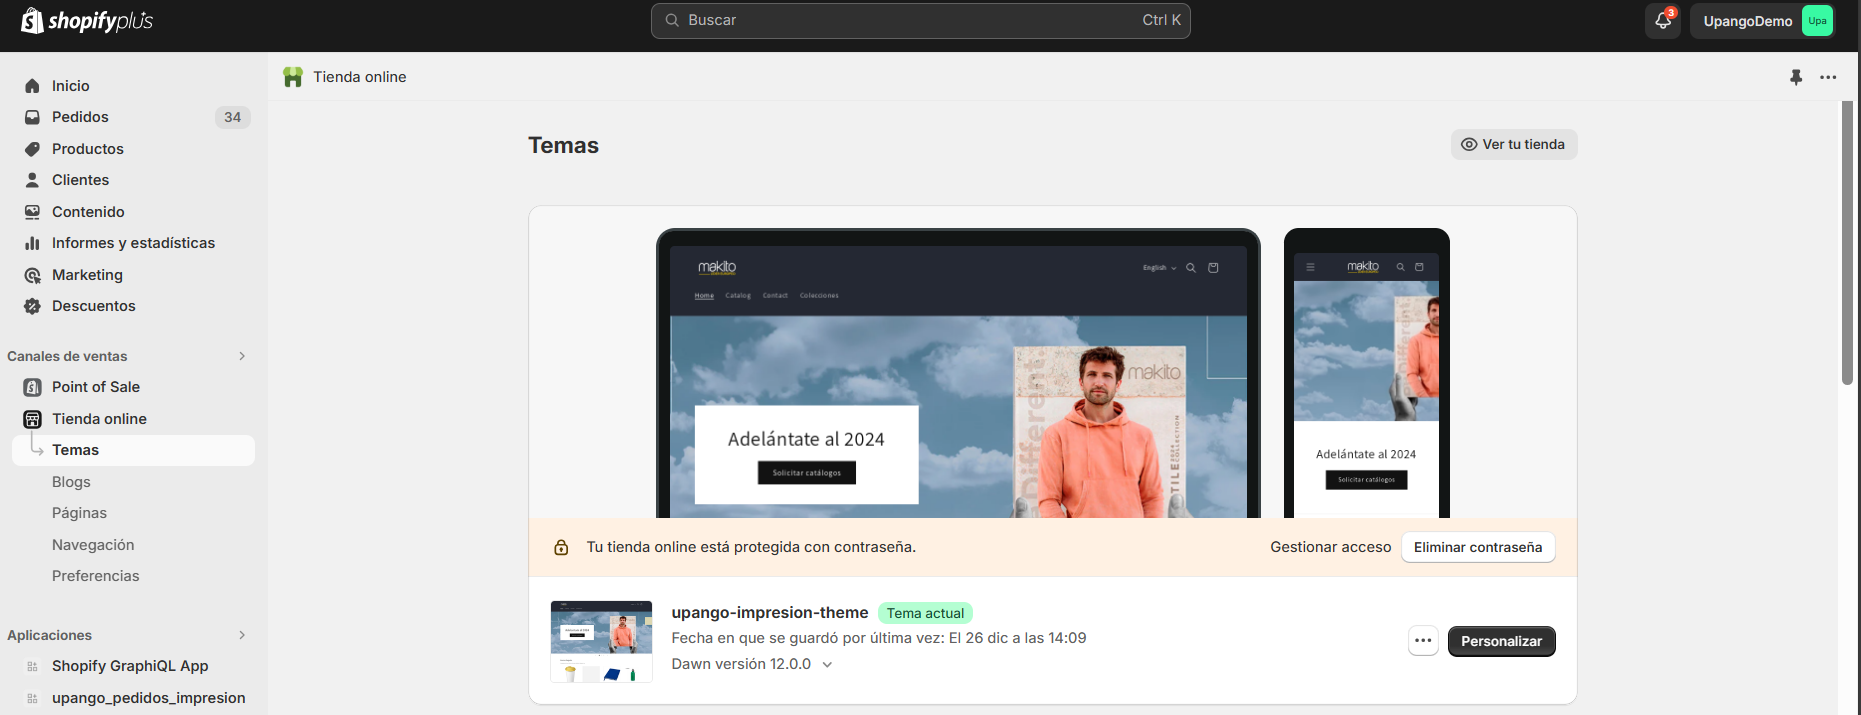
\includegraphics[width=0.8\textwidth]{imagenes/ManualUsuario/PantallaDePersonalizarTema.png}
    \caption{\label{fig:PersonalizarTema}Personalizar tema en el panel de administración}
    \vspace{\fill}
\end{figure}

Al instalar la app, se habilitan en el configurador todos aquellos componentes de tema que se han desarrollado en la aplicación.
En la Figura~\ref{fig:ThemeAppExtension} se puede observar la pantalla del configurador del tema, en ella el administrador deber ir a la plantilla de la página de producto y añadir
en el lugar que considere más apropiado el bloque que se ha desarrollado en la extensión de tema de la aplicación. Como puede verse, al instroducir este elemento, se muestra en la pantalla de producto
el botón para abrir el personalizador de artículos que lleva detrás toda la funcionalidad.

\begin{figure}[ht]
    \floatplacement{figure}{!t}
    \centering
    \includegraphics[width=0.8\textwidth]{imagenes/ManualUsuario/AñadirBloqueThemeExtension.png}
    \caption{\label{fig:ThemeAppExtension}Añadir la extensión de tema de la App en el tema de la tienda}
    \vspace{\fill}
\end{figure}

Una vez añadida la extensión del tema, hay que dirigirse a la pantalla del panel de administración que se ha desarrollado en la aplicación. En la Figura~\ref{fig:PanelAdministracion} se puede
ver un enlace a esta pantalla en la sección \textit{Aplicaciones} $\rightarrow$  \textit{upango\_pedidos\_impresion}. En la Figura~\ref{fig:FuncionalidadAdministracion} se observa dicha pantalla, en ella se puede pulsar el botón \textit{Crear Metadatos} para que se creen 
automáticamente los metacampos de producto necesarios, y el botón \textit{cart-transform} para que se cree automáticamente en la tienda el objeto cart-transform, el cuál hara uso de una función de la aplicación, que 
dotará al carrito y al checkout de la tienda de una funcionalidad y apariencia de paquetes customizados.

\begin{figure}[ht]
    \floatplacement{figure}{!t}
    \centering
    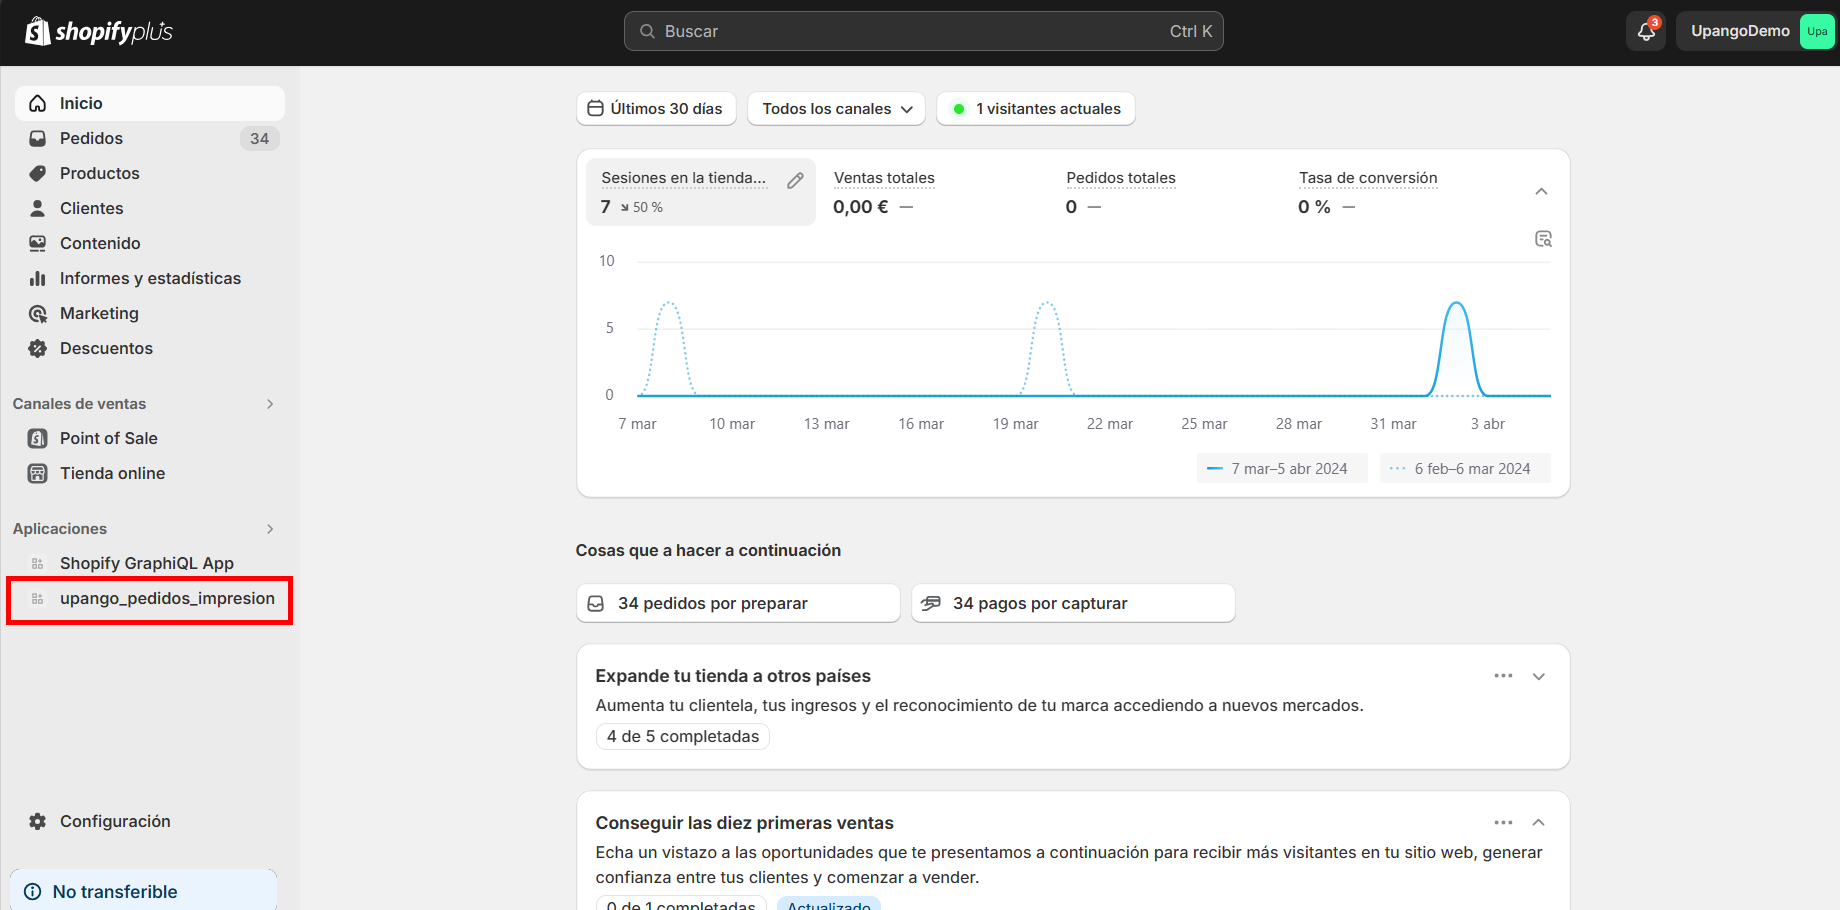
\includegraphics[width=0.8\textwidth]{imagenes/ManualUsuario/PaginaAdministracion.png}
    \caption{\label{fig:PanelAdministracion}Panel de administración de la tienda}
    \vspace{\fill}
\end{figure}

\begin{figure}[ht]
    \floatplacement{figure}{!t}
    \centering
    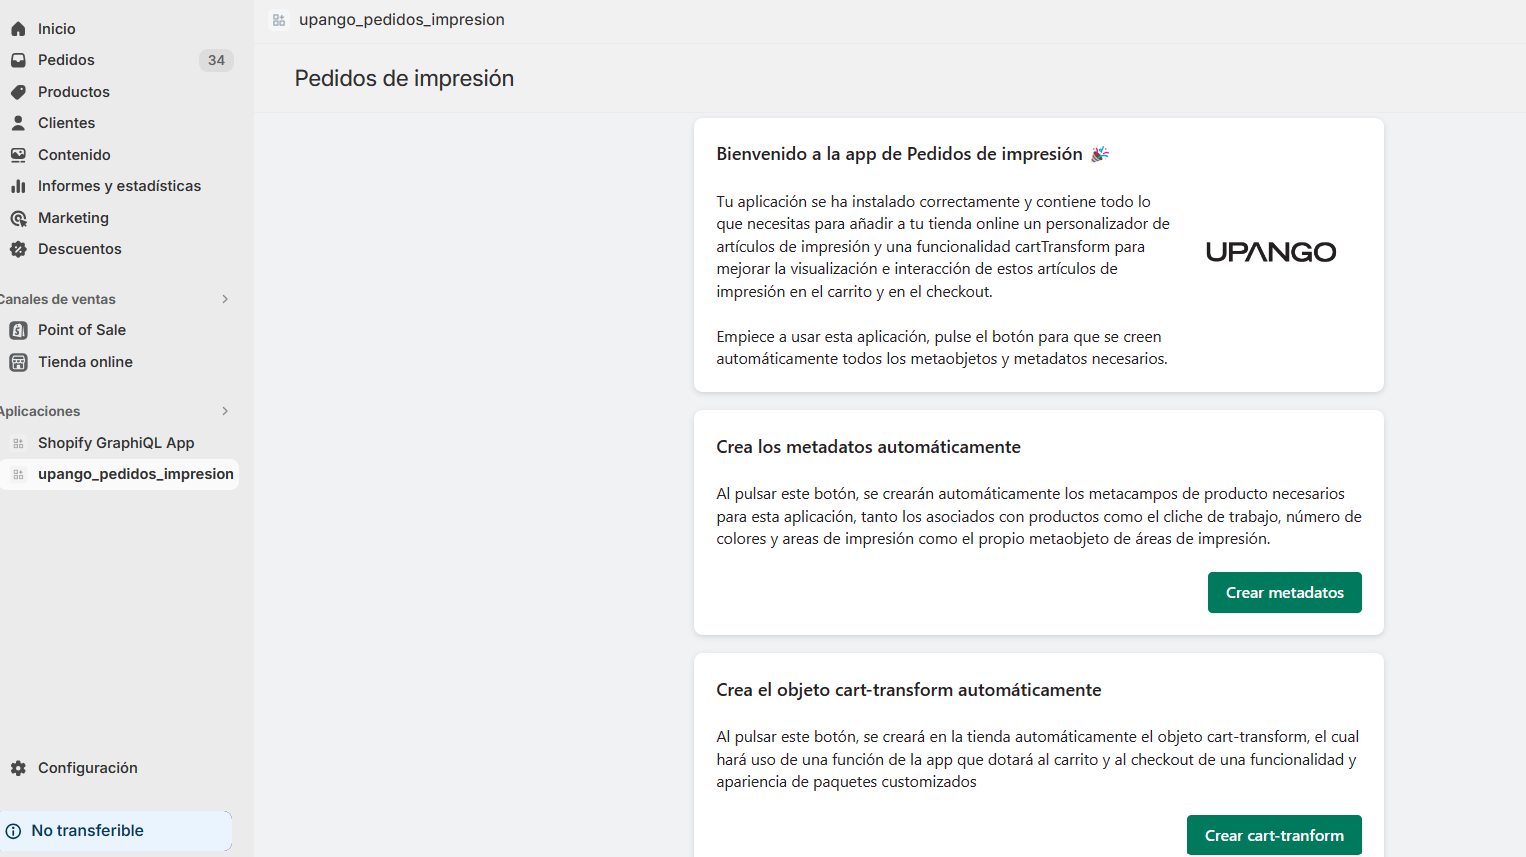
\includegraphics[width=0.8\textwidth]{imagenes/ManualUsuario/FuncionalidadPaginaAdministracion.png}
    \caption{\label{fig:FuncionalidadAdministracion}Funcionalidades de la parte de administración de la App}
    \vspace{\fill}
\end{figure}

Una vez realizadas estas configuraciones y creados en la tienda todos los productos necesarios, trabajos de impresión, tipos de cliche, asociados los productos con sus areas de impresión, y todos los elementos necesarios relacionados con
la impresión de artículos, ya se puede hacer uso de la tienda con las funcionalidades de personalización de productos integrada.

En la Figura~\ref{fig:HomeTiendaDemo} se puede observar la página principal de la tienda, en ella el usuario puede navegar hacia otros apartados de la tienda, como el catálogo de productos, se puede buscar secciones y productos con el buscador, ir al carrito, seleccionar el idioma y otras funcionalidades.También
es posible seleccionar cualquier producto de los que aparecen en destacados para ir a la página de producto y poder añadirlo al carrito o personalizarlo si se trata de un producto
personalizable.

\begin{figure}[ht]
    \floatplacement{figure}{!t}
    \centering
    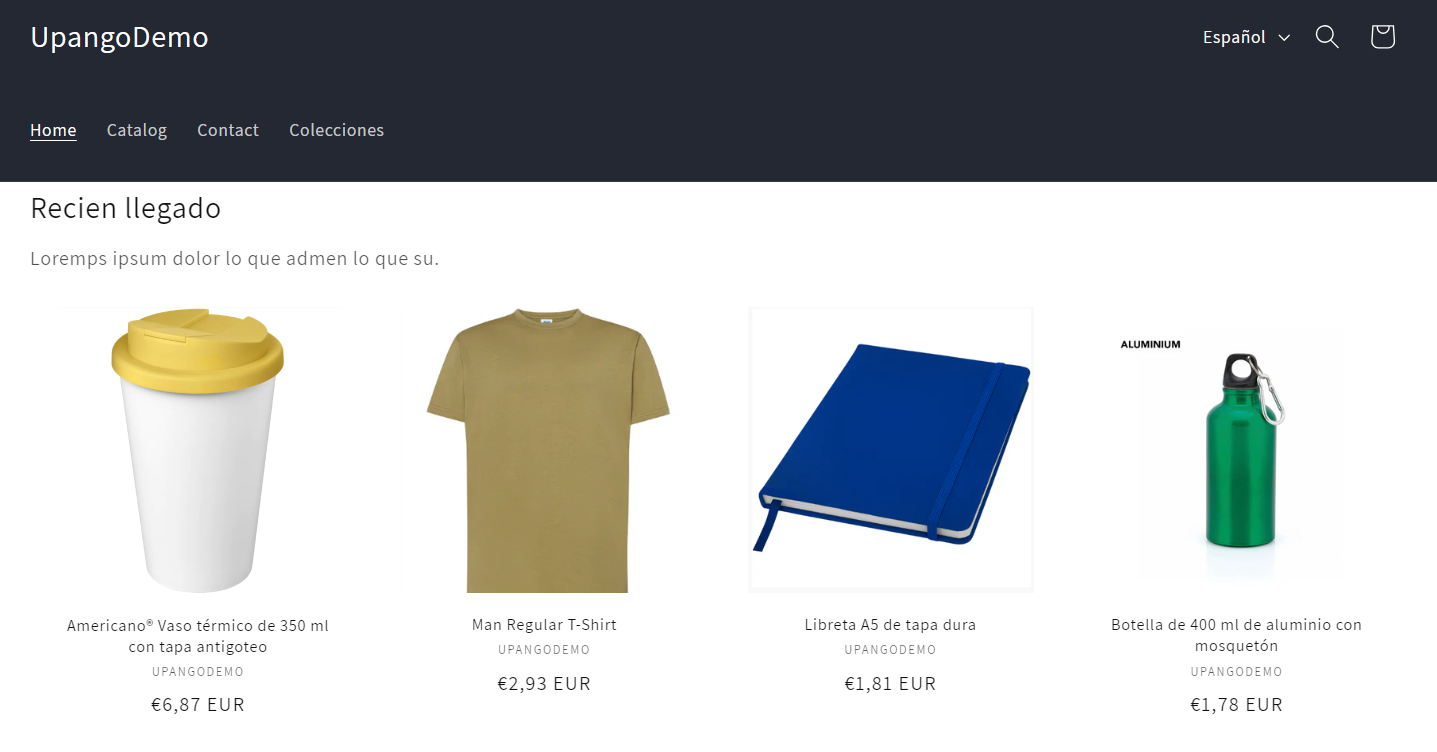
\includegraphics[width=0.8\textwidth]{imagenes/ManualUsuario/HomeTiendaDemo.png}
    \caption{\label{fig:HomeTiendaDemo}Página principal de la tienda de demostración}
    \vspace{\fill}
\end{figure}

En la imagen~\ref{fig:ProductoNoPersonalizable} se puede ver como se ha navegado hacia una página de producto. En esta, como puede observarse, no aparece el botón para personalizar este
artículo, lo que significa que el producto no es personalizable y en este caso solo se podría seleccionar la cantidad deseada y añadir al carrito o comprar directamente.
En la siguiente imagen (Figura~\ref{fig:ProductoPersonalizable}) se puede ver otra página de producto, y en este caso si aparece el botón de personalizar, lo que indica que este producto
si sería personalizable y cuenta con sus áreas de impresión correspondientes y todos sus atributos de personalización. En esta pantalla se puede comprar este producto y tratarlo como en el caso anterior,
y comprarlo sin personalización, o es posible seleccionar la cantidad que se desee y pulsar el botón de personalizar para configurar y añadir al carrito los productos a través de la interfaz de personalización.

\begin{figure}[ht]
    \floatplacement{figure}{!t}
    \centering
    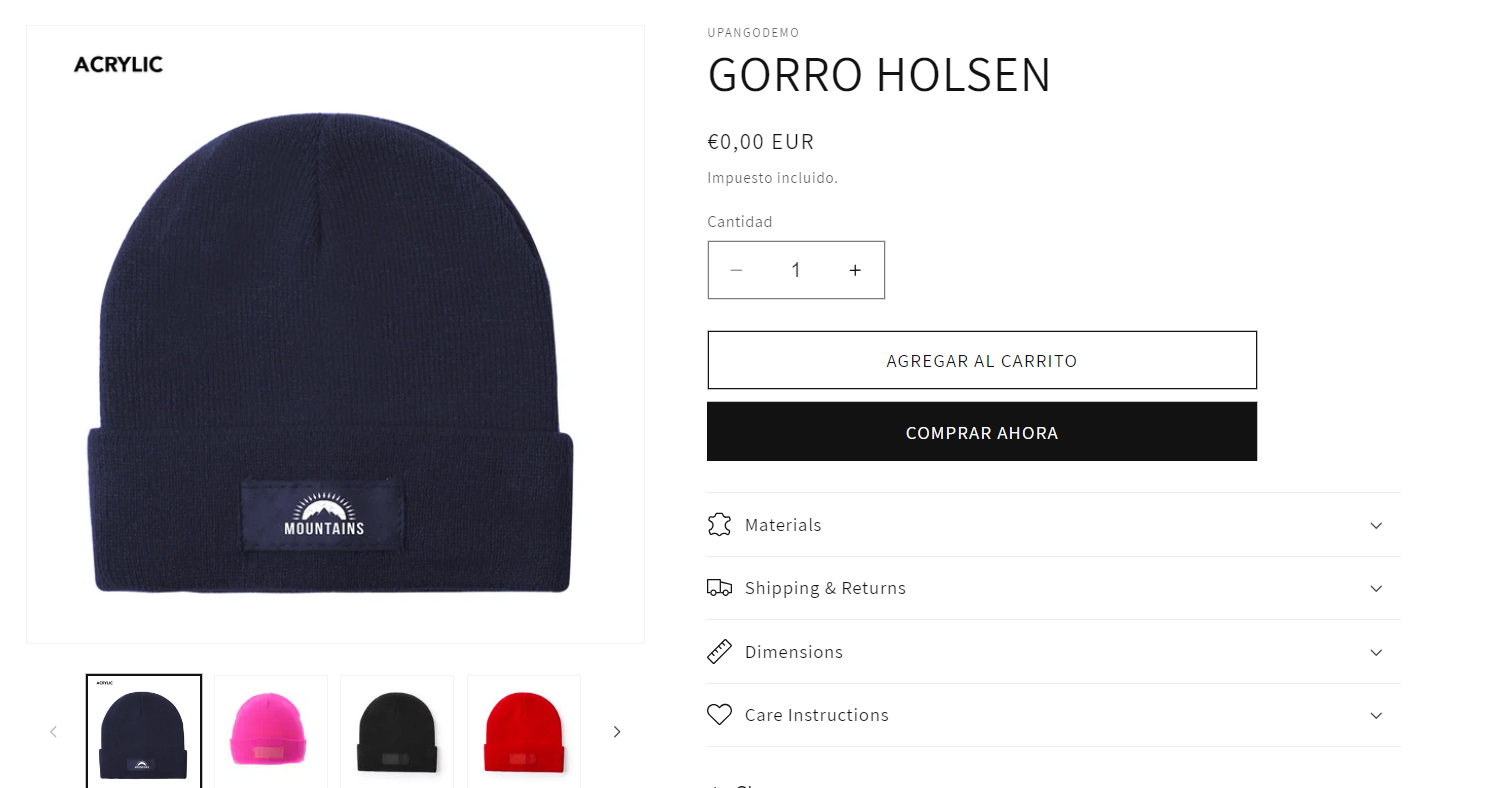
\includegraphics[width=0.8\textwidth]{imagenes/ManualUsuario/PaginaProductoSinPersonalizacion.png}
    \caption{\label{fig:ProductoNoPersonalizable}Página de producto no personalizable}
    \vspace{\fill}
\end{figure}

\begin{figure}[ht]
    \floatplacement{figure}{!t}
    \centering
    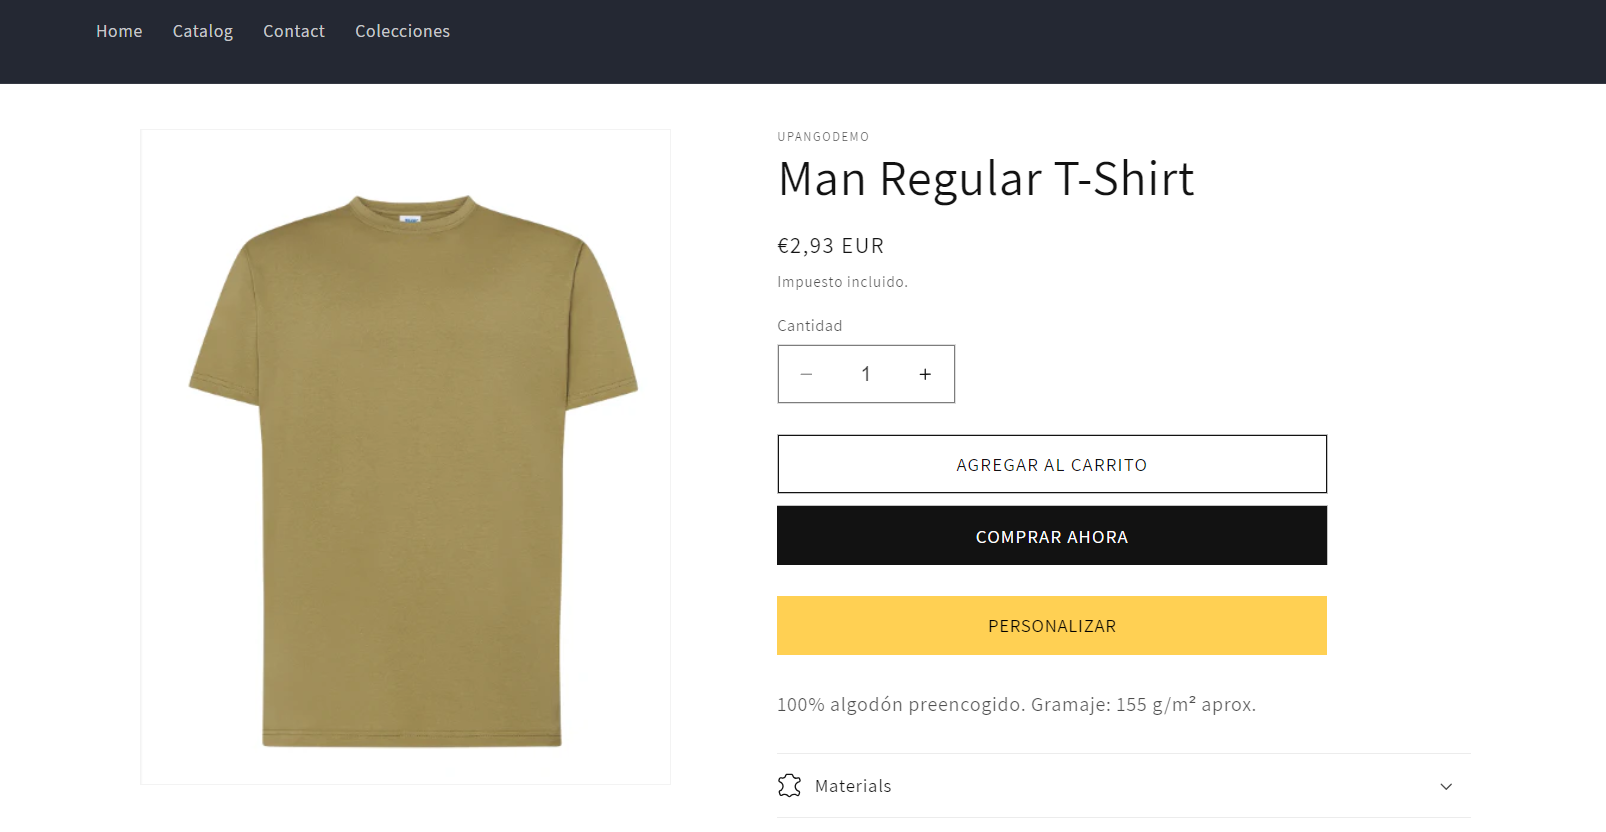
\includegraphics[width=0.8\textwidth]{imagenes/ManualUsuario/PaginaProductoConPersonalizacion.png}
    \caption{\label{fig:ProductoPersonalizable}Página de producto personalizable}
    \vspace{\fill}
\end{figure}

Si se pulsa en el botón de personalizar, se abrirá el personalizador de artículos. En este, como se puede ver en la Figura~\ref{fig:Personalizador}, se encuentran
las distintas areas de impresión con las que cuenta el producto con sus atributos personalizables y a la derecha se puede ir viendo el resumen del pedido presonalizado actualizado.
Como se puede observar, ahora mismo en el resumen del pedido solamente aparece el producto con las unidades, el precio por unidad y el precio total, pues todavía se ha seleccionado ni configurado
ningún area del producto.

\begin{figure}[ht]
    \floatplacement{figure}{!t}
    \centering
    \includegraphics[width=0.8\textwidth]{imagenes/ManualUsuario/PersonalizadorArtículosCamiseta.png}
    \caption{\label{fig:Personalizador}Pantalla del personalizador del producto seleccionado}
    \vspace{\fill}
\end{figure}

Si se selecciona un área de impresión, como se puede observar en la Figura~\ref{fig:PersonalizadorAreaMarcada}, se observa como se refresca el resumen de pedido y se le agrega tanto el trabajo de impresión
seleccionado por defecto, como su cliche asociado. Una vez seleccionada el área se pueden configurar todos los elementos que contiene. Además también permite seleccionar varias áreas en una misma personalización, como 
se puede ver en la Figura~\ref{fig:PersonalizadorVariasAreas}. En ella aparecen varias áreas del producto seleccionadas y en el resumen aparecen reflejados los trabajos y cliches de dichas áreas y su importe total.

\begin{figure}[ht]
    \floatplacement{figure}{!t}
    \centering
    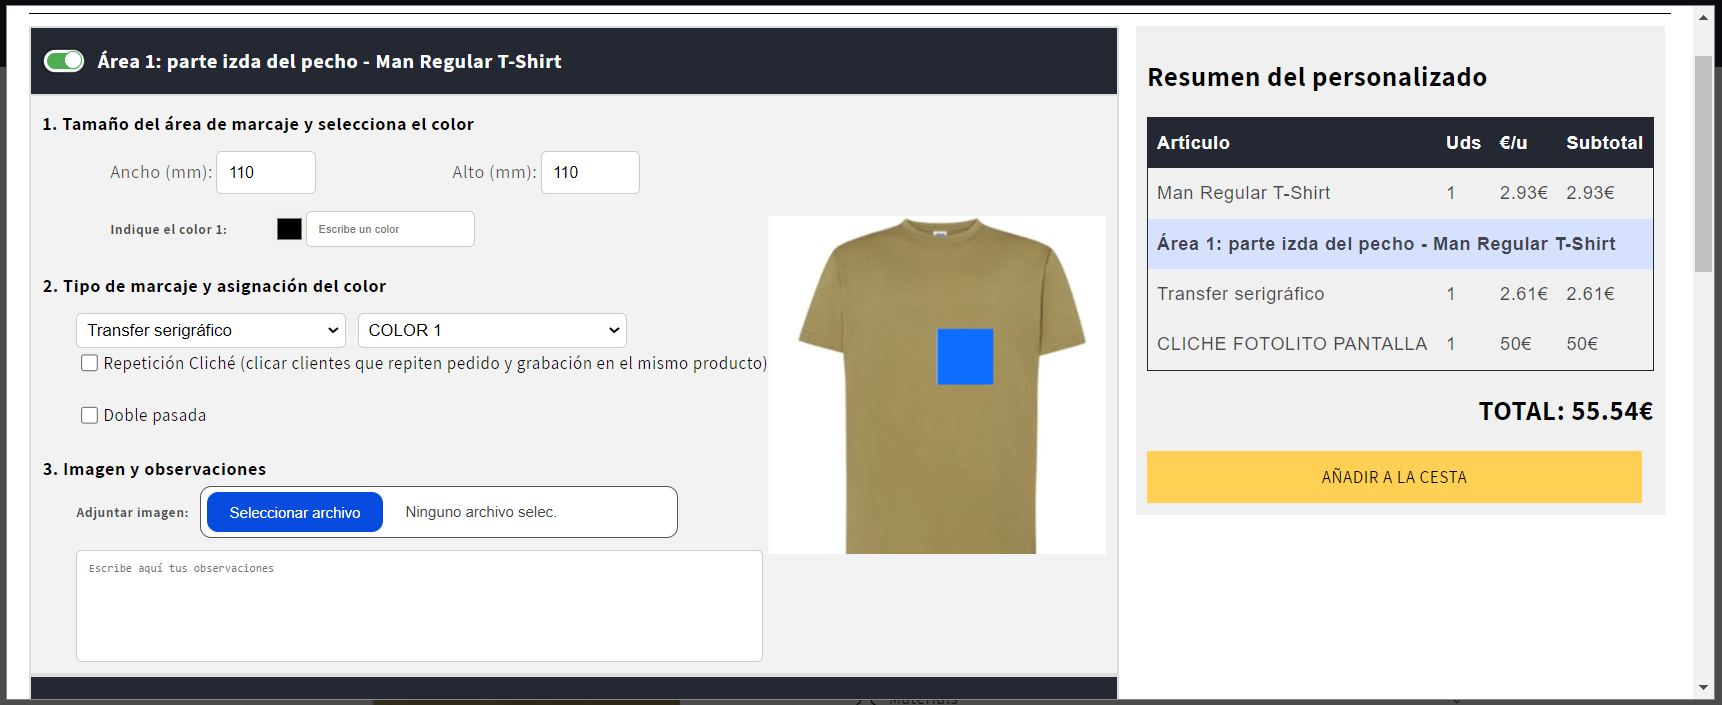
\includegraphics[width=0.8\textwidth]{imagenes/ManualUsuario/PersonalizadorArea1Seleccionada.png}
    \caption{\label{fig:PersonalizadorAreaMarcada}Personalizador con el Area 1 seleccionada}
    \vspace{\fill}
\end{figure}

\begin{figure}[ht]
    \floatplacement{figure}{!t}
    \centering
    \includegraphics[width=0.8\textwidth]{imagenes/ManualUsuario/PersonalizadorVariasAreasDeImpresiónSeleccionadas.png}
    \caption{\label{fig:PersonalizadorVariasAreas}Personalizador con varias áreas seleccionadas}
    \vspace{\fill}
\end{figure}

En cuanto a la configuración de cada área, como se puede apreciar en la Figura~\ref{fig:PersonalizadorColores}, existen un par de inputs para introducir las medidas de la impresión que se deseen 
realizar en el artículo, uno para el ancho y otro para el alto. Además se puede observar un select para seleccionar el tipo de trabajo a aplicar en el producto seleccionado, es decir el tipo de marcaje. El tipo de trabajo seleccionado
afectará al selector de colores de su derecha, pues cada trabajo de impresión cuenta con un número máximo de colores con los que puede trabajar, y al modificar el trabajo se renderizará automáticamente el selector de colores.
También hay unos inputs en los que se pueden introducir los colores con los que se desea que se realice la impresión, existen tantos inputs como colores se hayan seleccionado en el select de colores y estos
se refrescan al modificar el valor de ese select. En este caso se ha seleccionado el tipo de trabajo \textit{transfer serigráfico}, también se ha introducido que se desea una impresión en 3 colores y se han seleccionado dichos colores en los inputs.
En el resumen de pedido se puede observar como aparece el trabajo de impresión, su cliche asociado y un cargo extra por la adicción de 2 colores extra.

\begin{figure}[ht]
    \floatplacement{figure}{!t}
    \centering
    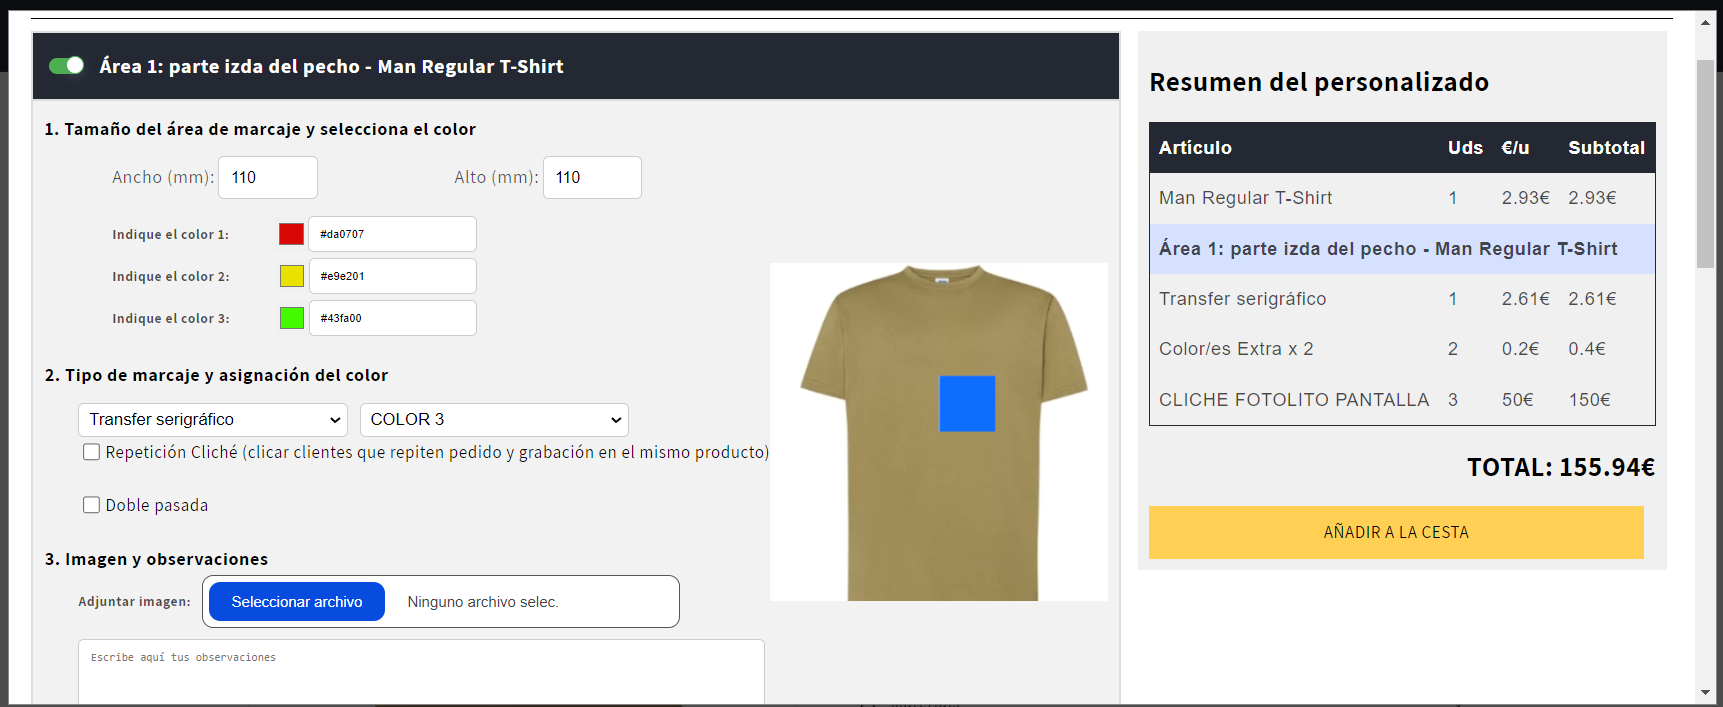
\includegraphics[width=0.8\textwidth]{imagenes/ManualUsuario/PersonalizadorArea1ColoresSeleccionados.png}
    \caption{\label{fig:PersonalizadorColores}Personalizador con trabajo de impresión y colores seleccionados}
    \vspace{\fill}
\end{figure}

En la personalización del área de impresión, también se pueden observar dos checks. Un check de repetición de cliche para marcar si ya se ha realizado algún otro pedido similar con el mismo tipo de impresión,
y otro check de doble pasada para indicar si se desea que la impresión se aplique dos veces. En la Figura~\ref{fig:PersonalizadorCheckboxes} se pueden apreciar estos dos checks marcados y como estos
afectan al precio total de impresión. En el resumen puede observarse como al haber marcado el check de repetición de cliche, el precio del cliche se ha reducido debido a que la empresa ahorraría costes al no tener que 
fabricar un nuevo cliche. Además al haber marcado el check de doble pasada se observa como en el resumen aparece un cargo extra por doble pasada.

\begin{figure}[ht]
    \floatplacement{figure}{!t}
    \centering
    \includegraphics[width=0.8\textwidth]{imagenes/ManualUsuario/PersonalizadorRepeticiónClicheDoblePasada.png}
    \caption{\label{fig:PersonalizadorCheckboxes}Personalizador con opciones de repetición de cliche y doble pasada}
    \vspace{\fill}
\end{figure}

También es posible seleccionar el logo que se desee imprimir en el producto. En la imagen~\ref{fig:PersonalizadorLogo} se observa como se ha seleccionado dicha imagen y se muestra de forma visual en el personalizador una 
aproximación de como quedaría ese logo impreso en la prenda que se desea comprar. Esta funcionalidad permite al cliente observar una imagen lo mas realista posible del resultado final
de la personalización del artículo. Además el cliente también puede introducir unas observaciones referidas a la personalización para dar mas detalles de la misma y tratar ciertos detalles que se puedan
estar escapando. Una vez personalizada la prenda, se puede pulsar el botón de añadir el carrito para añadir los productos con toda su personalización asociada y acorde con
lo visualizado en el resumen del pedido.

\begin{figure}[ht]
    \floatplacement{figure}{!t}
    \centering
    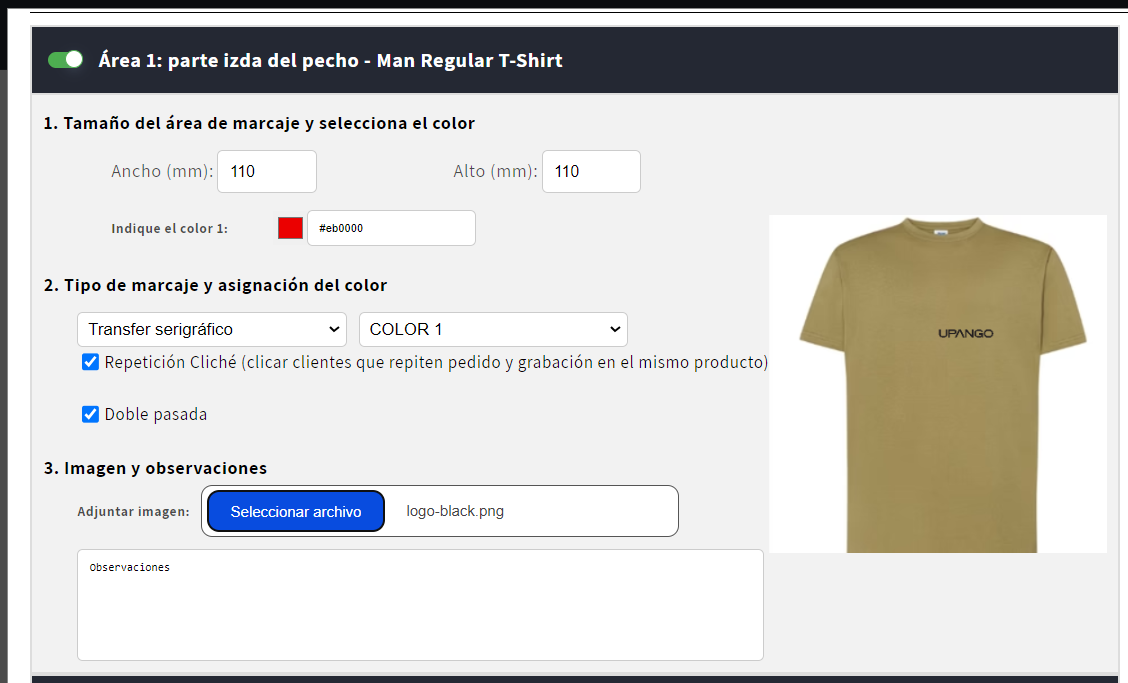
\includegraphics[width=0.8\textwidth]{imagenes/ManualUsuario/PersonalizadorLogoSeleccionado.png}
    \caption{\label{fig:PersonalizadorLogo}Personalizador con selección de logo}
    \vspace{\fill}
\end{figure}


Una vez añadido el producto personalizado al carrito se puede pulsar el botón de la cesta de la compra ubicado en la parte superior de la página (Figura~\ref{fig:BotonCarrito}), al pulsarlo se redirigiría a la página del carrito.
En dicha página (Figura~\ref{fig:Carrito}) se pueden observar los productos que han sido añadidos. Estos productos que han sido personalizados se añaden al carrito en forma de un solo paquete que contiene
tanto las unidades de los artículos, como todos los elementos y atributos de la personalización.
En la Figura~\ref{fig:Carrito} se observa un paquete de personalización que se ha añadido, en el cual se han seleccionado 3 unidades del producto, con el trabajo \textit{transfer serigráfico} y una serie de configuraciones 
que pueden verse mejor detalladas en la página del Checkout. Por último se puede pulsar el botón del carrito para completar la compra y se dirigiría al checkout donde se podrá completar el pedido.
Por último, en la Figura~\ref{fig:Checkout} se puede observar dicha interfaz para completar el proceso de compra, en la cual se puede visualizar con todo detalle el resumen de todo el pedido, introducir los datos de pago, facturación y dirección de envío
y completar el pedido.


\begin{figure}[ht]
    \floatplacement{figure}{!t}
    \centering
    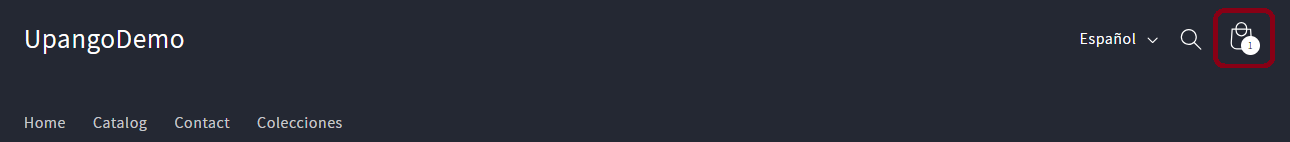
\includegraphics[width=0.8\textwidth]{imagenes/ManualUsuario/BotonCarrito.png}
    \caption{\label{fig:BotonCarrito}Botón de carrito}
    \vspace{\fill}
\end{figure}

\begin{figure}[ht]
    \floatplacement{figure}{!t}
    \centering
    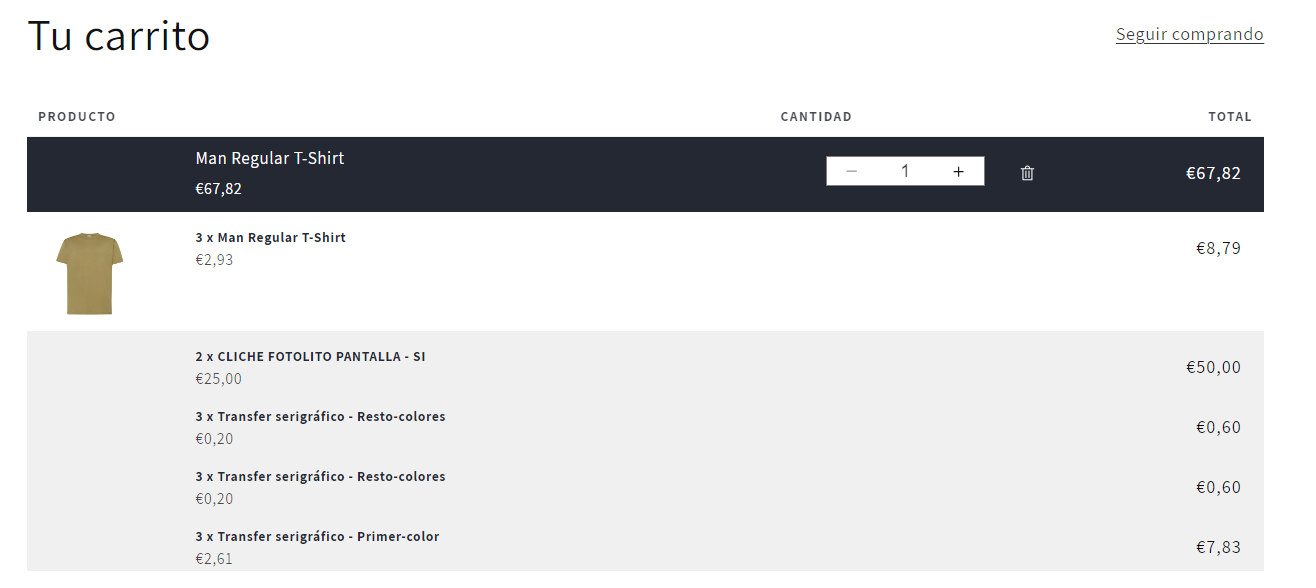
\includegraphics[width=0.8\textwidth]{imagenes/ManualUsuario/PantallaCarrito.png}
    \caption{\label{fig:Carrito}Pantalla del carrito de la tienda}
    \vspace{\fill}
\end{figure}

\begin{figure}[ht]
    \floatplacement{figure}{!t}
    \centering
    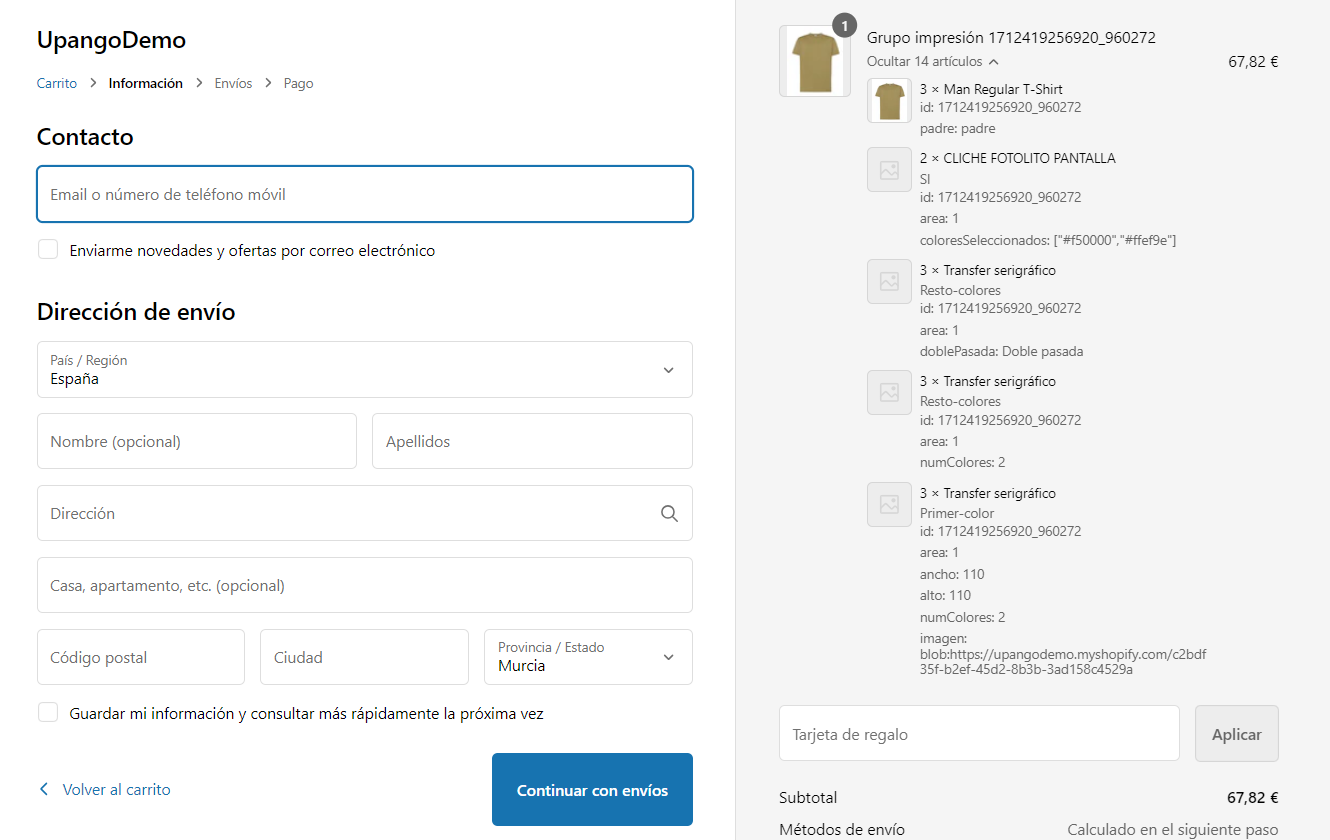
\includegraphics[width=0.8\textwidth]{imagenes/ManualUsuario/ImagenCheckout.png}
    \caption{\label{fig:Checkout}Pantalla de checkout de la tienda}
    \vspace{\fill}
\end{figure}


\end{document}

